% ============================================================================ %
%
%           Šablona bakalářské/diplomové práce
%
% Autor:    Ing. Jozef Říha (2006-05-04), od té doby šablonu udržuje
%           Ing. Pavel Tomášek, Ph.D. (tomasek@utb.cz)
%
% Verze:    2021-05-04
%
% Kódování: UTF-8 (kontrolní řetězec: žluťoučký kůň úpěl ďábelšké ódy)
%
% Sazba:    pdflatex prace.tex && pdflatex prace.tex
%           (nutné dvakrát pro korektní vložení citací a jiných referencí),
%           v případě umístění literatury do externího bib souboru je třeba volat
%           pdflatex prace.tex && bibtex prace && pdflatex prace.tex && pdflatex prace.tex
%
% Tip:      Ve správně vysázeném českém textu by na konci řádku neměla zůstant
%           samotná jednopísmenná předložka či spojka. Na takové místo se vkládá
%           nezalomitelná mezera pomocí symbolu ~. Existuje program, který umí
%           zpracovat celý TeX dokument najednou podle českých konvencí:
%           http://petr.olsak.net/ftp/olsak/vlna/
%
% Pozor:    Vzhledem k požadovanému standardu PDF/A nesmí vložené obrázky 
%           obsahovat alfa kanál (průhlednost).
%
% ============================================================================ %


\documentclass[a4paper,12pt]{article}

% Definice vzhledu a nastavení se načítá z následujícího souboru (netřeba editovat)
% ============================================================================ %
% Tento dokument není zpravidla třeba editovat,
% obsahuje nastavení balíčků, vzhledu, stylů.
%
% Kódování: UTF-8 (žluťoučký kůň úpěl ďábelšké ódy)
% ============================================================================ %


% ============================================================================ %
% BALÍČKY

%\usepackage[czech,english]{babel} % volba při kompilaci latexem (vyžaduje texlive-lang), zakomentovano, nastavovanu prikazem \nastavjazyk
\usepackage[T1]{fontenc}% definice vnitřního kódování
\usepackage[utf8x]{inputenc} % slouží pro definici kódování (při problémech zkusit zaměnit utf8x za utf8)
\usepackage{color}		% umožňuje použití barev
\usepackage{graphicx}	% rozšíření práce s grafikou
\usepackage{amsmath}	% balíček pro pokročilejší matematiku
\usepackage{fancyhdr}	% detailnější nastavení záhlaví a zápatí
\usepackage{tocloft}	% umožňuje pohodlné nastavení vzhledu obsahu, seznamu tabulek či obrázků
\usepackage{textcase}	% změna VeLiKoStI PíSmA
\usepackage{ifthen} 	% balíček umožňující skladby if, then -- využijeme při definici nadpisů
\usepackage{setspace}	% balíček umožňující nastavit řádkování na 1, 1.5, 2
\usepackage{ccaption}	% vylepšení práce s popisky obrázků či tabulek
\usepackage{sectsty}	% pro nastavení vzhledu nadpisů
\usepackage[srcstyle=leftnumhang,linenumbersep={\ }]{examplep} % pokročilejší sazba programového kódu
\usepackage{url}		% balíček pro vysázení internetové adresy stylem verbatim s vylepšeným řádkovým zlomem
\usepackage{afterpage}
%\usepackage{layout}	% zobrazí nastavení tiskového zrcadla (příkaz \layout)
%\usepackage{times}		% balíček pro použití fontu times
%\usepackage{verbatim}	% vysází text bez formátování, tak jak je zapsán v souboru
%\usepackage{indentfirst} % definuje odsazení prvního řádku odstavce
%\usepackage{makeidx}	% vytvoří rejstřík
\usepackage[pdftex,pdfa,hidelinks,breaklinks]{hyperref}	% vytváří křížové odkazy
%\usepackage{multicol}	% vícesloupcová sazba
%\usepackage{flafter}	% zajistí, aby se plovoucí objekty objevovali až za jejich umístěním v textu
\usepackage{chngcntr}	% Umožňuje změnu nastavení číslování obrázků, tabulek i rovnic
\usepackage{etoolbox}	% Tool-box for LaTeX programmers
\usepackage[labelsep=space,tableposition=bottom,justification=centering]{caption} % Přenastavení popisků u figur a tabulek
\usepackage{xmpincl}	% Pro aplikaci standardu PDF/A
\usepackage{hyperxmp}	% Pro aplikaci standardu PDF/A
\usepackage[final]{pdfpages}

%\pdfminorversion=4
%\pdfobjcompresslevel=0


% ---------------------------------------------------------------------------- %

% NASTAVENÍ TISKOVÉHO ZRCADLA

\newcommand{\valueTextHeight}{242mm}	% výška tiskového zrcadla
\newcommand{\valueTextWidth}{155mm}	% šířka tiskového zrcadla
\newcommand{\valueVOffset}{-1.61cm}	% vertikální posunutí tiskového zrcadla
\newcommand{\valueSideMargin}{0.96cm}	% levý okraj
\newcommand{\valueHeadHeight}{0.6cm}	% záhlaví
\newcommand{\valueHeadSep}{1cm}	% záhlaví

\textheight=\valueTextHeight
\textwidth=\valueTextWidth
\voffset=\valueVOffset
%\voffset=-1in
%\topmargin=-2.9cm

\oddsidemargin=\valueSideMargin
\evensidemargin=\valueSideMargin

\headheight=\valueHeadHeight
\headsep=\valueHeadSep

% nastavení zápatí
\footskip=1ex
\cfoot{}
% "vypnout" poznámky na okrajích
\marginparpush=0mm
\marginparwidth=0mm
\marginparsep=0mm

\pagestyle{fancy}

% Nastavení obalujících okrajů okolo popisků figur a tabulek
\captionsetup[figure]{aboveskip=5pt}
\captionsetup[figure]{belowskip=0pt}
\captionsetup[table]{aboveskip=0pt}
\captionsetup[table]{belowskip=5pt}


% ============================================================================ %
% NASTAVENÍ PÍSMA, ODSTAVCE, ROVNIC, POZNÁMEK

\parindent=0em				% velikost odstavcové zarážky na nulu
\def\thefootnote{\arabic{footnote})}	% poznámka pod čarou se závorkou
\onehalfspacing % nastavím řádkování tímto způsobem nebo \renewcommand{\baselinestretch}{1.5} ??
\setlength{\parskip}{3pt}		% vertikální mezera mezi nadpisy
%\def\label#1{{\sf ! #1 ! }}		% možnost zobrazení všech \label{}


% ============================================================================ %
% NASTAVENÍ ČÍTAČŮ

\setcounter{tocdepth}{3} % do obsahu se ukládají pouze první dvě úrovně kapitol


% ============================================================================ %
% PDF/A STANDARD

% http://www.mathstat.dal.ca/~selinger/pdfa/
% https://blog.zhaw.ch/icclab/creating-pdfa-documents-for-long-term-archiving/
% http://support.river-valley.com/wiki/index.php?title=Generating_PDF/A_compliant_PDFs_from_pdftex

% Prerequisites: pdflatex, hyperref, xmpincl
% pdfTeX at least in version 1.40.15 (in Linux add repository ppa:jonathonf/texlive, update and upgrade texlive-full)
%
% Validator: http://pdfa.k.utb.cz:8080/ https://www.pdf-online.com/osa/validate.aspx

% \convertDate converts D:20080419103507+02'00' to 2008-04-19T10:35:07+02:00
\def\convertDate{%
	\getYear
}
{\catcode`\D=12
 \gdef\getYear D:#1#2#3#4{\edef\xYear{#1#2#3#4}\getMonth}
}
\def\getMonth#1#2{\edef\xMonth{#1#2}\getDay}
\def\getDay#1#2{\edef\xDay{#1#2}\getHour}
\def\getHour#1#2{\edef\xHour{#1#2}\getMin}
\def\getMin#1#2{\edef\xMin{#1#2}\getSec}
\def\getSec#1#2{\edef\xSec{#1#2}\getTZh}
\def\getTZh +#1#2{\edef\xTZh{#1#2}\getTZm}
\def\getTZm '#1#2'{%
	\edef\xTZm{#1#2}%
	\edef\convDate{\xYear-\xMonth-\xDay T\xHour:\xMin:\xSec+\xTZh:\xTZm}%
}
\expandafter\convertDate\pdfcreationdate

\pdfminorversion 4

\immediate\pdfobj stream attr{/N 3} file{graphics/sRGBIEC1966-2.1.icm}
\pdfcatalog{%
	/OutputIntents [ <<
	/Type /OutputIntent
	/S/GTS_PDFA1
	/DestOutputProfile \the\pdflastobj\space 0 R
	/OutputConditionIdentifier (sRGB IEC61966-2.1)
	/Info(sRGB IEC61966-2.1)
 >> ]
}

\providecommand{\xmpOrg}{Tomas Bata University in Zlín, Czech Republic}
\providecommand{\xmpProducer}{}
\providecommand{\xmpDoi}{}
\providecommand{\xmpJournalnumber}{}
\providecommand{\xmpVolume}{}
\providecommand{\xmpIssue}{}
\providecommand{\xmpCoverDisplayDate}{}
\providecommand{\xmpCoverDate}{}
\providecommand{\xmpJournaltitle}{}
\providecommand{\xmpFirstpage}{}
\providecommand{\xmpLastpage}{}
\providecommand{\xmpAuthoritativeDomain}{}
\providecommand{\xmpCreatorTool}{}%pdfTeX

\newcommand{\aplikujpdfa}{
	\ifczech
		\providecommand{\xmpTitle}{\nazevcz}
		\providecommand{\xmpAuthor}{\autor}
		\providecommand{\xmpKeywords}{\klicovaslovacz}
		\hypersetup{
			pdftitle={\nazevcz},
			pdfauthor={\autor},
			pdfsubject={\abstraktcz},
			pdfkeywords={\klicovaslovacz},
			%pdfproducer={pdfTeX-1.40.20},
			pdflang=la,
			pdfapart=3,
			pdfaconformance=B,
			pdflang={cz}
		}
	\else \ifenglish
		\providecommand{\xmpTitle}{\nazeven}
		\providecommand{\xmpAuthor}{\autor}
		\providecommand{\xmpKeywords}{\klicovaslovaen}
		\hypersetup{
			pdftitle={\nazeven},
			pdfauthor={\autor},
			pdfsubject={\abstrakten},
			pdfkeywords={\klicovaslovaen},
			%pdfproducer={pdfTeX-1.40.20},
			pdflang=la,
			pdfapart=3,
			pdfaconformance=B,
			pdflang={en}
		}
	\fi \fi
	
	\makeatletter
	\includexmp{tex/pdfa-1b}
	\makeatother
}


% ============================================================================ %
% UŽIVATELSKÉ STYLY

% Styl nn = nečíslovaný nadpis (je vysázený v obsahu)
\def\nn#1{\clearpage\phantomsection\addcontentsline{toc}{section}{#1}\section*{\MakeTextUppercase{#1}}}

% Styl nm = nečíslovaný nadpis (není vysázený v obsahu)
\def\nm#1{\clearpage\section*{\MakeTextUppercase{#1}}}

% Styl ns = nečíslovaný nadpis na stejné stránce (není vysázený v obsahu)
\def\nns#1{\section*{\MakeTextUppercase{#1}}}

% Styl n{ur}{nadp} pro nadpisy, kde ur je číslo úrovně a nadp je text nadpisu
\def\n#1#2{
	
	\ifthenelse{#1=1}{
		\sectionfont{\normalsize\MakeUppercase}
		\clearpage\section{#2}
		\sectionfont{\normalsize}
		}{
		\ifthenelse{#1=2}{\subsection{#2}}{
			\ifthenelse{#1=3}{\subsubsection{#2}}{\paragraph{\itshape\bfseries{#2}}
}}}}

% Styl pro obrázky
% \obr{popisek}{label}{rozměr (0.0 - 1.0)}{soubor}
\def\obr#1#2#3#4{
	\begin{figure}[h]
		\centering
		\includegraphics[width=#3\linewidth]{#4}
		%\captionwidth{#3\linewidth}
		%\changecaptionwidth
		\captionsetup{width=#3\linewidth}
		\caption{#1}
		\label{#2}
	\end{figure}
}

% Styl pro tabulky
% \tab{popisek}{label}{rozměr (0.0 - 1.0)}{definice sloupců}{obsah} 
\def\tab#1#2#3#4#5{
	\begin{table}[h]
		%\captionwidth{#3\linewidth}
		%\changecaptionwidth
		\captionsetup{width=#3\linewidth}
		\caption{#1}
		\label{#2}
		\centering
		\begin{tabular}{#4}
			#5
		\end{tabular}
	\end{table}
}

% Styl pro tabulky v příloze
% \tabpri{popisek}{definice sloupců}{data tabulky}
\def\tabpri#1#2#3{
	\begin{table}[h]
	\begin{center}
	#1
	\end{center}
	\begin{center}
	\begin{tabular}{#2}
	#3
	\end{tabular}
	\end{center}
	\end{table}
}
	
% Styl pro tabulky z MS Excelu exportované do EPS
% \extab{popisek}{rozměr (0.0 - 1.0)}{soubor}
\def\extab#1#2#3{
	\begin{table}
	%\captionwidth{#2\linewidth}
	%\changecaptionwidth
	\captionsetup{width=#2\linewidth}
	\caption{#1}
	\begin{center}
	\includegraphics[width=#2\linewidth]{#3}
	\end{center}
	\end{table}
}

% Styl pro rovnice
% \rov[klíčové slovo]{rovnice}
\newcommand{\rov}[2][chybejici rovnice]{
	\begin{equation}
	#2
	\label{#1}
	\end{equation}
}
	
% Příkaz pro vysázení seznamu obrázků
\def\seznamobr{
	\clearpage
	\phantomsection
	\ifczech
		\addcontentsline{toc}{section}{Seznam obrázků}
	\else \ifenglish
		\addcontentsline{toc}{section}{List of Figures}
	\fi \fi
	\listoffigures
	\clearpage
}

% Příkaz pro vysázení seznamu tabulek
\def\seznamtab{
	\clearpage
	\phantomsection
	\ifczech
		\addcontentsline{toc}{section}{Seznam tabulek}
	\else \ifenglish
		\addcontentsline{toc}{section}{List of Tables}
	\fi \fi
	\listoftables
	\clearpage
}

\newcommand{\OdsazovaniOdstavcuStart}[0]{
	\ifenglish
		\setlength{\parskip}{5mm} % English indentation of paragraphs
	\else \ifczech
		\setlength{\parindent}{5mm} % Czech indentation of paragraphs
	\fi \fi
}

\newcommand{\OdsazovaniOdstavcuStop}[0]{
	\ifenglish
		\setlength{\parskip}{0mm} % English indentation of paragraphs
	\else \ifczech
		\setlength{\parindent}{0mm} % Czech indentation of paragraphs
	\fi \fi
}

% Příkaz pro vysázení seznamu literatury
\newcommand{\seznamlit}[1]{
	\clearpage
	\phantomsection
	\ifczech
		\addcontentsline{toc}{section}{Seznam použité literatury}
	\else \ifenglish
		\addcontentsline{toc}{section}{References}
	\fi \fi
	\begin{thebibliography}{99}
	#1
	\end{thebibliography}
}

\newcommand{\seznamlitbib}{
	\bibliographystyle{\ifenglish tex/czechiso-en\else\ifczech tex/czechiso-cz\fi\fi} % Respects the norm of ČSN ISO 690
	\newpage
	\clearpage
	%\cleardoublepage
	\phantomsection
	\addcontentsline{toc}{section}{\ifenglish References \else \ifczech Seznam použité literatury \fi \fi}
	\bibliography{tex/literatura}
}

% Příkaz pro přípravu seznamu použitých zkratek a symbolů
\newcommand{\seznamzkr}{
	\ifczech
		\nn{Seznam použitých symbolů a zkratek}
	\else \ifenglish
		\nn{List of Abbreviations}
	\fi \fi
}

% Příkaz \cast jako alternativa k \part
\def\cast#1{
	\clearpage
	\part{#1}
}

% Příkaz \obsah vysází obsah v daném místě
\def\obsah{
	\deaktivujZahlavi
	\clearpage
	\thispagestyle{empty}
	\tableofcontents
	\clearpage
	\pagestyle{fancy}
	\aktivujZahlavi
}

% Zkrácení stylu \textbf na \b
\def\b#1{
	\textbf{#1}
}

% \bi = tučná kurzíva
\newcommand{\bi}[1]{\textbf{\textit{#1}}}

% \it = kurzíva
\renewcommand{\it}[1]{\textit{#1}}

% Nastaveni nezobrazovani zahlavi dokumentu
\newcommand{\deaktivujZahlavi}{
	\lhead{}
	\rhead{}
	\renewcommand{\headrulewidth}{0pt}
}

\newcommand{\zadani}{
	% \clearpage
	% \thispagestyle{empty}
	% \voffset=\valueVOffset\evensidemargin=\valueSideMargin\oddsidemargin=\valueSideMargin\headsep=\valueHeadSep\headheight=\valueHeadHeight\setlength{\parskip}{3pt}\textheight=\valueTextHeight\textwidth=\valueTextWidth
	% *** Nascanované zadání, strana 1 ***
	
	% \clearpage
	% \thispagestyle{empty}
	% *** Nascanované zadání, strana 2 ***
	\voffset=\valueVOffset\evensidemargin=\valueSideMargin\oddsidemargin=\valueSideMargin\headsep=\valueHeadSep\headheight=\valueHeadHeight\setlength{\parskip}{3pt}\textheight=\valueTextHeight\textwidth=\valueTextWidth
	\includepdf[pages=-]{zadani.pdf}
	%\includepdf[pages=1-2, pagecommand={}, trim=1cm 2cm 1cm 2cm, clip]{~/School/Thesis/Thesis/tex/zadani.pdf}
}

% Nastaveni zobrazovani zahlavi dokumentu
\newcommand{\aktivujZahlavi}{
	\renewcommand{\headrulewidth}{1pt}
	\rhead{\thepage}
	
	\ifczech
		\lhead{\b{UTB ve Zlíně, \ifthenelse{\equal{\fakulta}{FAI}}{Fakulta aplikované informatiky}{\ifthenelse{\equal{\fakulta}{FAME}}{Fakulta managementu a ekonomiky}{\ifthenelse{\equal{\fakulta}{FHS}}{Fakulta humanitních studií}{\ifthenelse{\equal{\fakulta}{FLKR}}{Fakulta logistiky a krizového řízení}{\ifthenelse{\equal{\fakulta}{FMK}}{Fakulta multimediálních komunikací}{\ifthenelse{\equal{\fakulta}{FT}}{Fakulta technologická}{\ifthenelse{\equal{\fakulta}{UNI}}{Univerzitní institut}{}}}}}}}}}
	\else \ifenglish
		\lhead{\b{TBU in Zlín, \ifthenelse{\equal{\fakulta}{FAI}}{Faculty of Applied Informatics}{\ifthenelse{\equal{\fakulta}{FAME}}{Faculty of Management and Economics}{\ifthenelse{\equal{\fakulta}{FHS}}{Faculty of Humanities}{\ifthenelse{\equal{\fakulta}{FLKR}}{Faculty of Logistics and Crisis Management}{\ifthenelse{\equal{\fakulta}{FMK}}{Faculty of Multimedia Communications}{\ifthenelse{\equal{\fakulta}{FT}}{Faculty of Technology}{\ifthenelse{\equal{\fakulta}{UNI}}{University Institute}{}}}}}}}}}
	\fi \fi
}

% Příkaz \logopracerok vloží na dané místo logo fakulty, typ práce a rok
\newcommand{\logopracerok}{
	\ifczech
		\iffai	\put(82.2,-223.3){\makebox(84,16.4){
\includegraphics[width=90mm]{graphics/logo/fai_logo_cz.png}}} \fi
		\iffame	\put(82.2,-223.3){\makebox(84,16.4){
\includegraphics[width=90mm]{graphics/logo/fame_logo_cz.png}}} \fi
		\iffhs	\put(82.2,-223.3){\makebox(84,16.4){
\includegraphics[width=90mm]{graphics/logo/fhs_logo_cz.png}}} \fi
		\ifflkr	\put(82.2,-223.3){\makebox(84,16.4){
\includegraphics[width=90mm]{graphics/logo/flkr_logo_cz.png}}} \fi
		\iffmk	\put(82.2,-223.3){\makebox(84,16.4){
\includegraphics[width=90mm]{graphics/logo/fmk_logo_cz.png}}} \fi
		\ifft	\put(82.2,-223.3){\makebox(84,16.4){
\includegraphics[width=90mm]{graphics/logo/ft_logo_cz.png}}} \fi
		\ifuni	\put(82.2,-223.3){\makebox(84,16.4){
\includegraphics[width=90mm]{graphics/logo/uni_logo_cz.png}}} \fi
	\else \ifenglish
		\iffai	\put(82.2,-223.3){\makebox(84,16.4){
\includegraphics[width=90mm]{graphics/logo/fai_logo_en.png}}} \fi
		\iffame	\put(82.2,-223.3){\makebox(84,16.4){
\includegraphics[width=90mm]{graphics/logo/fame_logo_en.png}}} \fi
		\iffhs	\put(82.2,-223.3){\makebox(84,16.4){
\includegraphics[width=90mm]{graphics/logo/fhs_logo_en.png}}} \fi
		\ifflkr	\put(82.2,-223.3){\makebox(84,16.4){
\includegraphics[width=90mm]{graphics/logo/flkr_logo_en.png}}} \fi
		\iffmk	\put(82.2,-223.3){\makebox(84,16.4){
\includegraphics[width=90mm]{graphics/logo/fmk_logo_en.png}}} \fi
		\ifft	\put(82.2,-223.3){\makebox(84,16.4){
\includegraphics[width=90mm]{graphics/logo/ft_logo_en.png}}} \fi
		\ifuni	\put(82.2,-223.3){\makebox(84,16.4){
\includegraphics[width=90mm]{graphics/logo/uni_logo_en.png}}} \fi
	\fi \fi
	\put(0,-205){\linethickness{1pt}\line(1,0){170}}
	\ifczech
		\ifbp \put(4,-215){\makebox(69.5,4.5)[l]{\noindent\fontsize{16}{1}\usefont{OT1}{phv}{m}{n}Bakalářská práce}} \fi
		\ifdp \put(4,-215){\makebox(69.5,4.5)[l]{\noindent\fontsize{16}{1}\usefont{OT1}{phv}{m}{n}Diplomová práce}} \fi
	\else \ifenglish
		\ifbp \put(4,-215){\makebox(69.5,4.5)[l]{\noindent\fontsize{16}{1}\usefont{OT1}{phv}{m}{n}Bachelor's thesis}} \fi
		\ifdp \put(4,-215){\makebox(69.5,4.5)[l]{\noindent\fontsize{16}{1}\usefont{OT1}{phv}{m}{n}Master's thesis}} \fi
	\fi \fi
	\put(4,-220){\makebox(69.5,4.5)[l]{\noindent\fontsize{16}{1}\usefont{OT1}{phv}{m}{n}\rok}}
	\put(0,-225){\linethickness{1pt}\line(1,0){170}}
	\put(75,-223.3){\linethickness{1pt}\line(0,1){16.4}}
}

% Úvodní stránka s logem fakulty
\newcommand{\titulnistrana}{
	\thispagestyle{empty}
	\voffset=-2.01cm\evensidemargin=0pt\oddsidemargin=0cm\parindent=0pt\headsep=0pt\headheight=0pt\parskip=0pt\textheight=272mm\textwidth=200mm
	\renewcommand{\baselinestretch}{0}
	
	\setlength{\unitlength}{1mm}
	\begin{picture}(-10,8)
		\ifczech
			% Nazev prace
			%\put(0,-100){\makebox(170,50){\fontsize{24}{1}\usefont{OT1}{phv}{b}{n}#1}}
			%		\put(0,-100){\makebox(170,50){\protect\parbox{0.8\textwidth}{\protect\centering\fontsize{24}{1}\usefont{OT1}{phv}{b}{n}#1}}}
			
			% Vyreseno odradkovani
			\put(0,-100){\makebox(170,50){\protect\parbox{0.8\textwidth}{\protect\centering\setstretch{2.0}\usefont{OT1}{phv}{b}{n}{\Huge\nazevcz}}}}
			
			% Jmeno autora
			\put(0,-135){\makebox(170,25){\fontsize{20}{1}\usefont{OT1}{phv}{m}{n}\autor}}
		\else \ifenglish
			% Nazev prace
			%\put(0,-100){\makebox(170,50){\fontsize{24}{1}\usefont{OT1}{phv}{b}{n}#1}}
			%\put(0,-95){\makebox(170,50){\protect\parbox{0.8\textwidth}{\protect\centering\fontsize{24}{1}\usefont{OT1}{phv}{b}{n}#1}}}
			%\put(0,-88)%toto bylo pouzito v pripade zobrazeni nazvu ve dvou jazycich
			\put(0,-100){\makebox(170,50){\protect\parbox{0.8\textwidth}{\protect\centering\setstretch{2.0}\usefont{OT1}{phv}{b}{n}{\Huge\nazeven}}}}
	
			%\put(0,-111){\makebox(170,50){\fontsize{20}{1}\usefont{OT1}{phv}{m}{n}#1}}
			%\put(0,-116){\makebox(170,50){\protect\parbox{0.8\textwidth}{\protect\centering\fontsize{20}{1}\usefont{OT1}{phv}{m}{n}#2}}}
			%\put(0,-115){\makebox(170,50){\protect\parbox{0.8\textwidth}{\protect\centering\setstretch{1.5}\usefont{OT1}{phv}{m}{n}{\Large\nazevcz}}}}
			
			% Jmeno autora
			\put(0,-135){\makebox(170,25){\fontsize{20}{1}\usefont{OT1}{phv}{m}{n}\autor}}
		\fi \fi
		\logopracerok
	\end{picture}
}


% Strana s abstraktem a klíčovými slovy v češtině a angličtině
\newcommand{\abstraktaklicovaslova}{
	\clearpage
	\thispagestyle{empty}
	\nm{Abstrakt}
	\abstraktcz
	
	\vspace{1cm}
	Klíčová slova: \klicovaslovacz
	
	\vspace{3cm}
	
	\nns{Abstract}
	\abstrakten
	
	\vspace{1cm}
	Keywords: \klicovaslovaen
}


% ============================================================================ %
% NASTAVENÍ ZOBRAZENÍ PŘÍLOH -- SEZNAM, ČÍSLOVÁNÍ, VLASTNÍ STYL

\makeatletter % tímto příkazem dávám najevo, že budu editovat přímo příkazy ze šablony

% definice seznamu příloh - příkaz \listofappendices
\def\listofappendices{%
	\newpage
	\phantomsection
	\setcounter{section}{0}
	\ifczech
		\addcontentsline{toc}{section}{Seznam příloh}
		\@restonecolfalse\if@twocolumn\@restonecoltrue\onecolumn\fi
		\section*{SEZNAM PŘÍLOH}
	\else \ifenglish
		\addcontentsline{toc}{section}{List of Appendices}
		\@restonecolfalse\if@twocolumn\@restonecoltrue\onecolumn\fi
		\section*{LIST OF APPENDICES}
	\fi \fi
	\@mkboth{LIST OF APPENDICES}{LIST OF APPENDICES}
	\@starttoc{loa}\if@restonecol\twocolumn\fi
	\pagestyle{empty}
	\thispagestyle{fancy}
}

\def\ext@appendix{loa}
\def\tocname{loa}

% definice příkazu \priloha{nazev prilohy} pro vložení nové přílohy
\newcommand{\priloha}[1]{
	\clearpage
	\refstepcounter{section}
	%\voffset=-3cm % vertikalni posun
	\addtocontents{loa}{\protect\makebox[1.5cm][l]{\ifczech P\else \ifenglish A\fi\fi\ \@Roman\c@section.} #1\newline}
	\ifczech
		{\bf PŘÍLOHA \ifczech P\else \ifenglish A\fi\fi\ \@Roman\c@section. \MakeTextUppercase{#1}}
	\else \ifenglish
		{\bf APPENDIX \ifczech P\else \ifenglish A\fi\fi\ \@Roman\c@section. \MakeTextUppercase{#1}}
	\fi \fi
	\par
}

% ============================================================================ %
% OBSAH: NASTAVENÍ VELKÝCH PÍSMEN PRO NÁZVY SEKCÍ A HLAVNÍCH NADPISŮ

\let\oldcontentsline\contentsline
\def\contentsline#1#2{%
	\expandafter\ifx\csname l@#1\endcsname\l@section
		\expandafter\@firstoftwo
	\else
		\expandafter\@secondoftwo
	\fi
	{%
		\oldcontentsline{#1}{\MakeTextUppercase{#2}}%
	}{%
		\oldcontentsline{#1}{#2}%
	}%
}

\def\@part[#1]#2{
	\ifnum \c@secnumdepth >\m@ne
		\refstepcounter{part}
		\addcontentsline{toc}{section}{\protect\texorpdfstring{\makebox[0.85cm]{\thepart\hfill} #1}{\thepart\ #1}}
	\else
		\addcontentsline{toc}{section}{#1}
	\fi
	{\parindent \z@ \raggedright
	\interlinepenalty \@M
	\clearpage
	\normalfont
	\ifnum \c@secnumdepth >\m@ne
		\Large\bfseries
		\nobreak
	\fi
	\vspace*{9cm}
	\center\huge \bfseries\thepart. \MakeTextUppercase{#2}
	\markboth{}{}\par}
	\nobreak
	\clearpage
	\@afterheading
}


% ============================================================================ %
% NASTAVENÍ FORMÁTU ČÍSLOVÁNÍ OBRÁZKŮ A TABULEK

\def\thefigure{\arabic{figure}}	% číslování obrázků typu (y)
\def\thetable{\arabic{table}}	% číslování tabulek typu (y)
\captiondelim{. } % změníme dvoutečku za Obr/Tab za tečku

% Nastavení číslování obrázků, tabulek i rovnic do formátu <číslo kapitoly>.<pořadové číslo>
\counterwithin{figure}{section}
\counterwithin{table}{section}
\counterwithin{equation}{section}

% Odsazeni popisku v seznamu obrazku a tabulek
\patchcmd{\@caption}{\csname the#1\endcsname}{\csname fnum@#1\endcsname}{}{}
%{\renewcommand*\numberline[1]{Fig. \,#1\space}}
%\renewcommand*\l@figure{\@dottedtocline{1}{0em}{5.0em}}
%\renewcommand*\l@table{\@dottedtocline{1}{0em}{5.0em}}

% Vynulování čítačů
\@addtoreset{table}{section}
\@addtoreset{figure}{section}
\@addtoreset{footnote}{section}

\makeatother % a to je ukončení \makeatletter


% ============================================================================ %
% ÚPRAVA VZHLEDU OBSAHU, SEZNAMU OBRÁZKŮ A TABULEK

% nastavení vertikální mezery před stylem část, nadpis 1--3
\setlength{\cftbeforepartskip}{3pt}
\setlength{\cftbeforesecskip}{3pt}
\setlength{\cftbeforesubsecskip}{3pt}
\setlength{\cftbeforesubsubsecskip}{0cm}

% odsazení zleva pro styl část, nadpis 1--3
\setlength{\cftpartindent}{0cm}
\setlength{\cftsecindent}{0cm}
\setlength{\cftsubsecindent}{0cm}
\setlength{\cftsubsubsecindent}{0cm}

% nastavení fontu pro styl část, nadpis 1--3
\renewcommand{\cftpartfont}{\small\bfseries}
\renewcommand{\cftsecfont}{\small\bfseries}
\renewcommand{\cftsubsecfont}{\scshape}
\renewcommand{\cftsubsubsecfont}{}

% odsazení čísla a textu titulku pro styl část, nadpis 1--3
\cftsetindents{part}{0cm}{1cm}
\cftsetindents{sec}{0cm}{1cm}
\cftsetindents{subsec}{0.5cm}{1.25cm}
\cftsetindents{subsubsec}{1cm}{1.5cm}
\cftsetindents{fig}{0cm}{1.5cm}
\cftsetindents{tab}{0cm}{1.5cm}

% nastavení vodící čáry pro styl část, nadpis 1--3, obrázky a tabulky
\renewcommand{\cftdot}{\ensuremath{.}} % tímto příkazem lze změnit vodící tečky v obsahu na jiný znak
\renewcommand{\cftpartleader}{\cftdotfill{0.3}}
\renewcommand{\cftsecleader}{\cftdotfill{0.3}}
\renewcommand{\cftsubsecleader}{\cftdotfill{0.3}}
\renewcommand{\cftsubsubsecleader}{\cftdotfill{0.3}}
\renewcommand{\cftfigleader}{\cftdotfill{0.3}}
\renewcommand{\cfttableader}{\cftdotfill{0.3}}

% změna fontu pro text "Obsah", "Seznam obrázků" a "Seznam tabulek"
\renewcommand{\cfttoctitlefont}{\normalsize\bfseries\thispagestyle{empty}}
\renewcommand{\cftloftitlefont}{\normalsize\bfseries\thispagestyle{fancy}}
\renewcommand{\cftlottitlefont}{\normalsize\bfseries\thispagestyle{fancy}}

\renewcommand{\cfttabpresnum}{Tab. }
\renewcommand{\cftfigaftersnum}{.}
\renewcommand{\cfttabaftersnum}{.}
\setlength{\cftfignumwidth}{5em}
\setlength{\cfttabnumwidth}{5em}


% ============================================================================ %
% NASTAVENÍ FONTU PRO NADPISY

\sectionfont{\normalsize}
\subsectionfont{\normalsize\bfseries}
\subsubsectionfont{\small\bfseries}
\paragraphfont{\small\bf}

% definice nového stylu \comment -- komentář k šabloně
\newcommand{\comment}[1]{\color{red}#1\color{black}}


% ============================================================================ %
% VSTUPY

% Nastaveni a kontrola fakulty
\newcommand{\nastavfakultu}[1]{
	\newcommand{\fakulta}{#1}
	\newif\iffai	\let\iffai\iffalse
	\newif\iffame	\let\iffame\iffalse
	\newif\iffhs	\let\iffhs\iffalse
	\newif\ifflkr	\let\ifflkr\iffalse
	\newif\iffmk	\let\iffmk\iffalse
	\newif\ifft		\let\ifft\iffalse
	\newif\ifuni	\let\ifuni\iffalse
	
	\ifthenelse{\equal{#1}{FAI}}{\let\iffai\iftrue}{}
	\ifthenelse{\equal{#1}{FAME}}{\let\iffame\iftrue}{}
	\ifthenelse{\equal{#1}{FHS}}{\let\iffhs\iftrue}{}
	\ifthenelse{\equal{#1}{FLKR}}{\let\ifflkr\iftrue}{}
	\ifthenelse{\equal{#1}{FMK}}{\let\iffmk\iftrue}{}
	\ifthenelse{\equal{#1}{FT}}{\let\ifft\iftrue}{}
	\ifthenelse{\equal{#1}{UNI}}{\let\ifuni\iftrue}{}
	
	\iffai \else \iffame \else \iffhs \else \ifflkr \else \iffmk \else \ifft \else \ifuni \else
		\errmessage{Chyba nastaveni fakulty}
	\fi \fi \fi \fi \fi \fi \fi
}

% Nastaveni a kontrola typu prace
\newcommand{\nastavtyp}[1]{
	\newcommand{\typ}{#1}
	
	\newif\ifbp \let\ifbp\iffalse
	\newif\ifdp \let\ifdp\iffalse
	
	\ifthenelse{\equal{#1}{BP}}{\let\ifbp\iftrue}{}
	\ifthenelse{\equal{#1}{DP}}{\let\ifdp\iftrue}{}
	
	\ifbp \else \ifdp \else
		\errmessage{Chyba nastaveni typu prace}
	\fi \fi
}

% Nastaveni roku
\newcommand{\nastavrok}[1]{
	\newcommand{\rok}{#1}
}

% Nastaveni jmena
\newcommand{\nastavautora}[1]{
	\newcommand{\autor}{#1}
}

% Nastaveni nazvu
\newcommand{\nastavnazevcz}[1]{
	\newcommand{\nazevcz}{#1}
}
\newcommand{\nastavnazeven}[1]{
	\newcommand{\nazeven}{#1}
}

% Nastaveni abstraktu
\newcommand{\nastavabstraktcz}[1]{
	\newcommand{\abstraktcz}{#1}
}
\newcommand{\nastavabstrakten}[1]{
	\newcommand{\abstrakten}{#1}
}

% Nastaveni klicovych slov
\newcommand{\nastavklicovaslovacz}[1]{
	\newcommand{\klicovaslovacz}{#1}
}
\newcommand{\nastavklicovaslovaen}[1]{
	\newcommand{\klicovaslovaen}{#1}
}

% Nastaveni a kontrola jazyka
\newcommand{\nastavjazyk}[1]{
	\newcommand{\jazyk}{#1}
	
	\newif\ifczech		\let\ifczech\iffalse
	\newif\ifenglish	\let\ifenglish\iffalse
	
	\ifthenelse{\equal{#1}{CZ}}{\let\ifczech\iftrue}{}
	\ifthenelse{\equal{#1}{EN}}{\let\ifenglish\iftrue}{}
	
	\ifczech \else \ifenglish \else
		\errmessage{Chyba nastaveni jazyka}
	\fi \fi
	
	\ifczech
		\usepackage[czech]{babel}
		% Vlastni definice nazvu
		\addto\captionsczech{\renewcommand{\contentsname}{\MakeTextUppercase{Obsah}}}
		\addto\captionsczech{\renewcommand{\refname}{\MakeTextUppercase{Seznam použité literatury}}}
		\addto\captionsczech{\renewcommand{\listfigurename}{\MakeTextUppercase{Seznam obrázků}}}
		\addto\captionsczech{\renewcommand{\listtablename}{\MakeTextUppercase{Seznam tabulek}}}
		%\addto\captionsczech{\renewcommand{\figurename}{Obr.}}
		%\addto\captionsczech{\renewcommand{\tablename}{Tab.}}
		\renewcommand{\cftfigpresnum}{Obr. }
	\else \ifenglish
		\usepackage[english]{babel}	
		% Vlastni definice nazvu
		\addto\captionsenglish{\renewcommand{\contentsname}{\MakeTextUppercase{Table of Contents}}}
		\addto\captionsenglish{\renewcommand{\refname}{\MakeTextUppercase{References}}}
		\addto\captionsenglish{\renewcommand{\listfigurename}{\MakeTextUppercase{List of Figures}}}
		\addto\captionsenglish{\renewcommand{\listtablename}{\MakeTextUppercase{List of Tables}}}
		%\addto\captionsenglish{\renewcommand{\figurename}{Fig.}}
		%\addto\captionsenglish{\renewcommand{\tablename}{Tab.}}
		\renewcommand{\cftfigpresnum}{Fig. }
	\fi \fi
}


% Nastaveni vertikalniho odsazeni nad rovnicemi/soustavami rovnic (prvni parametr),
% a pod (druhy parametr)
\newcommand{\nastavmezerukolemrovnic}[2]{
	\let\oldequation=\equation
	\let\endoldequation=\endequation
	\renewenvironment{equation}{\vspace{#1}\begin{oldequation}}{\end{oldequation}\vspace{#2}}
	
	\let\oldeqnarray=\eqnarray
	\let\endoldeqnarray=\endeqnarray
	\renewenvironment{eqnarray}{\vspace{#1}\begin{oldeqnarray}}{\end{oldeqnarray}\vspace{#2}}
}

% Nastaveni vertikalniho odsazeni nad tabulkami (prvni parametr),
% a pod (druhy parametr)
\newcommand{\nastavmezerukolemtabulek}[2]{
	\let\oldtable=\table
	\let\endoldtable=\endtable
	\renewenvironment{table}{\vspace{#1}\begin{oldtable}}{\end{oldtable}\vspace{#2}}
}

% Nastaveni vertikalniho odsazeni nad obrazky (prvni parametr),
% a pod (druhy parametr)
\newcommand{\nastavmezerukolemobrazku}[2]{
	\let\oldfigure=\figure
	\let\endoldfigure=\endfigure
	\renewenvironment{figure}{\vspace{#1}\begin{oldfigure}}{\end{oldfigure}\vspace{#2}}
}


% ============================================================================ %
% STRANA S PROHLASENIM

\newcommand{\prohlaseni}{{
	\clearpage
	\thispagestyle{empty}

	\ifczech
	\textbf{Prohlašuji, že}
	\begin{itemize}
		\setlength{\parskip}{0pt}
		\setlength{\itemsep}{0pt}
		\setstretch{1.05}
		\item{beru na vědomí, že odevzdáním \ifbp bakalářské \else \ifdp diplomové \fi \fi práce souhlasím se zveřejněním své práce podle zákona č. 111/1998 Sb. o vysokých školách a o změně a doplnění dalších zákonů (zákon o vysokých školách), ve znění pozdějších právních předpisů, bez ohledu na výsledek obhajoby;}
		\item{beru na vědomí, že \ifbp bakalářské \else \ifdp diplomové \fi \fi práce bude uložena v elektronické podobě v univerzitním informačním systému dostupná k prezenčnímu nahlédnutí, že jeden výtisk \ifbp bakalářské \else \ifdp diplomové \fi \fi práce bude uložen v příruční knihovně \iffai Fakulty aplikované informatiky. \else \iffame Fakulty managementu a ekonomiky. \else \iffhs Fakulty humanitních studií. \else \ifflkr Fakulty logistiky a krizového řízení. \else \iffmk Fakutly mutimediálních komunikací. \else \ifft Fakulty technologické. \else \ifuni Univerzitního institutu. \if \fi \fi \fi \fi \fi \fi \fi \fi Univerzity Tomáše Bati ve Zlíně; }
		\item{byl/a jsem seznámen/a s tím, že na moji \ifbp bakalářskou \else \ifdp diplomovou \fi \fi práci se plně vztahuje zákon č. 121/2000 Sb. o právu autorském, o právech souvisejících s právem autorským a o změně některých zákonů (autorský zákon) ve znění pozdějších právních předpisů, zejm. § 35 odst. 3;}
		\item{beru na vědomí, že podle § 60 odst. 1 autorského zákona má Univerzita Tomáše Bati ve Zlíně právo na uzavření licenční smlouvy o užití školního díla v rozsahu § 12 odst. 4 autorského zákona;}
		\item{beru na vědomí, že podle § 60 odst. 2 a 3 autorského zákona mohu užít své dílo –\ \ifbp bakalářskou \else \ifdp diplomovou \fi \fi práci nebo poskytnout licenci k~jejímu využití jen připouští-li tak licenční smlouva uzavřená mezi mnou a Univerzitou Tomáše Bati ve Zlíně s~tím, že vyrovnání případného přiměřeného příspěvku na úhradu nákladů, které byly Univerzitou Tomáše Bati ve Zlíně na vytvoření díla vynaloženy (až do jejich skutečné výše) bude rovněž předmětem této licenční smlouvy;}
		\item{beru na vědomí, že pokud bylo k vypracování \ifbp bakalářské \else \ifdp diplomové \fi \fi práce využito softwaru poskytnutého Univerzitou Tomáše Bati ve Zlíně nebo jinými subjekty pouze ke~studijním a výzkumným účelům (tedy pouze k~nekomerčnímu využití), nelze výsledky \ifbp bakalářské \else \ifdp diplomové \fi \fi práce využít ke komerčním účelům;}
		\item{beru na vědomí, že pokud je výstupem \ifbp bakalářské \else \ifdp diplomové \fi \fi práce jakýkoliv softwarový produkt, považují se za součást práce rovněž i zdrojové kódy, popř. soubory, ze kterých se projekt skládá. Neodevzdání této součásti může být důvodem k~neobhájení práce.}
	\end{itemize}
	\medskip
	%\clearpage
	%\thispagestyle{empty}
	\textbf{Prohlašuji,}
	\begin{itemize}
		\setlength{\parskip}{0pt}
		\setlength{\itemsep}{0pt}
		\setstretch{1.05}
		\item{že jsem na \ifbp bakalářské \else \ifdp diplomové \fi \fi práci pracoval samostatně a použitou literaturu jsem citoval. V případě publikace výsledků budu uveden jako spoluautor.}
		\item{že odevzdaná verze \ifbp bakalářské \else \ifdp diplomové \fi \fi práce a verze elektronická nahraná do IS/STAG jsou totožné.}
	\end{itemize}
	\medskip
	Ve Zlíně, dne \hspace{6.5cm}\dots\dots\dots\dots\dots\dots\dots\dots\dots\dots
	
	\hspace{10.3cm}podpis studenta
	
	\else \ifenglish
	%\nm{THESIS AUTHOR STATEMENT}
	\textbf{I hereby declare that:}
	\begin{itemize}
		\setlength{\parskip}{0pt}
		\setlength{\itemsep}{0pt}
		\setstretch{1.05}
		\item{I understand that by submitting my \ifbp Bachelor's \else\ifdp Master's \fi\fi thesis, I agree to the publication of my work according to Law No. 111/1998, Coll., On Universities and on changes and amendments to other acts (e.g. the Universities Act), as amended by subsequent legislation, without regard to the results of the defence of the thesis.}		
		\item{I understand that my \ifbp Bachelor's \else\ifdp Master's \fi\fi Thesis will be stored electronically in the university information system and be made available for on-site inspection, and that a copy of the \ifbp Bachelor's \else\ifdp Master's \fi\fi Thesis will be stored in the Reference Library of the 
		\iffai Faculty of Applied Informatics, \else\iffame Faculty of Management and Economics, \else \iffhs Faculty of Humanities, \else\ifflkr Faculty of Logistics and Crisis Management, \else\iffmk Faculty of Multimedia Communications, \else\ifft Faculty of Technology, \else\ifuni University Institute, \if \fi \fi \fi \fi \fi \fi \fi \fi Tomas Bata University in Zlín.}
		\item{I am aware of the fact that my \ifbp Bachelor's \else\ifdp Master's \fi\fi Thesis is fully covered by Act No. 121/2000 Coll. On Copyright, and Rights Related to Copyright, as amended by some other laws (e.g. the Copyright Act), as amended by subsequent legislation; and especially, by §35, Para. 3.}
		\item{I understand that, according to §60, Para. 1 of the Copyright Act, Tomas Bata University in Zlín has the right to conclude licensing agreements relating to the use of scholastic work within the full extent of §12, Para. 4, of the Copyright Act.}
		\item{I understand that, according to §60, Para. 2, and Para. 3, of the Copyright Act, I may use my work – \ifbp Bachelor's \else\ifdp Master's \fi\fi Thesis, or grant a license for its use, only if permitted by the licensing agreement concluded between myself and Tomas Bata University in Zlín with a view to the fact that Tomas Bata University in Zlín must be compensated for any reasonable contribution to covering such expenses/costs as invested by them in the creation of the thesis (up until the full actual amount) shall also be a subject of this licensing agreement.}
		\item{I understand that, should the elaboration of the \ifbp Bachelor's \else\ifdp Master's \fi\fi Thesis include the use of software provided by Tomas Bata University in Zlín or other such entities strictly for study and research purposes (i.e. only for non-commercial use), the results of my \ifbp Bachelor's \else\ifdp Master's \fi\fi Thesis cannot be used for commercial purposes.}
		\item{I understand that, if the output of my \ifbp Bachelor's \else\ifdp Master's \fi\fi Thesis is any software product(s), this/these shall equally be considered as part of the thesis, as well as any source codes, or files from which the project is composed. Not submitting any part of this/these component(s) may be a reason for the non-defence of my thesis.}
	\end{itemize}
	\medskip
	%\clearpage
	%\thispagestyle{empty}
	\textbf{I herewith declare that:}
	\begin{itemize}
		\setlength{\parskip}{0pt}
		\setlength{\itemsep}{0pt}
		\setstretch{1.05}
		\item{I have worked on my thesis alone and duly cited any literature I have used. In the case of the publication of the results of my thesis, I shall be listed as co-author.}
		\item{The submitted version of the thesis and its electronic version uploaded to IS/STAG are both identical.}
	\end{itemize}
	\medskip
	In Zlín; dated: \hspace{6.5cm}\dots\dots\dots\dots\dots\dots\dots\dots\dots\dots

	\hspace{10.3cm}Student's Signature
	
	\fi \fi
}}

% ============================================================================ %


% Uživatelské definice -- upravte dle požadavků
\nastavfakultu{FAI}
	% FAI  -- pro Fakultu aplikované informatiky
	% FAME -- pro Fakultu managementu a ekonomiky
	% FHS  -- pro Fakultu humanitních studií
	% FLKR -- pro Fakultu logistiky a krizového řízení
	% FMK  -- pro Fakutlu mutimediálních komunikací
	% FT   -- pro Fakultu technologickou
	% UNI  -- pro Univerzitní institut
\nastavtyp{DP}
	% BP   -- bakalářská práce
	% DP   -- diplomová práce
\nastavrok{2024}
	% zadejte rok místo "xxxx"
\nastavjazyk{CZ}
	% CZ   -- práce bude v českém jazyce
	% EN   -- práce bude v anglickém jazyce

% Lze přidat vertikalni odsazeni nad (prvni parametr) a pod (druhy parametr)
% obrázky, tabulky i rovnice/soustavy rovnic
\nastavmezerukolemobrazku{0mm}{0mm}
\nastavmezerukolemtabulek{0mm}{0mm}
\nastavmezerukolemrovnic{0mm}{0mm}

\nastavautora{Bc. Noe Švanda}
\nastavnazevcz{Analýza služeb kompilovaných v režimu Ahead-of-Time a Just-In-Time na platformě .NET}
\nastavnazeven{Název práce anglicky (max. 2 řádky)} % Jen u anglicky psané práce
\nastavabstraktcz{Tato diplomová práce analyzuje možnosti kompilace služeb v režimu Ahead-of-Time a Just-In-Time na platformě .NET. Zaměřuje se na srovnání vývojového procesu, výstupu a výkonu služeb kompilovaných v obou režimech. Za tímto účelem je vytvořena aplikace pro testování scénářů a monitorování výsledků. Výsledkem práce je analýza vývojového postupu, programového výstupu a výkonnostních dat služeb. Na jejich základě jsou porovnány výhody a nevýhody obou režimů kompilace a analyzována jejich použitelnost.}
\nastavabstrakten{This thesis analyses the possibilities of compiling services in Ahead-of-Time and Just-In-Time mode on the .NET platform. It focuses on comparing the development process, output and performance of services compiled in both modes. To this end, an application is created to test the scenarios and monitor the results. The result of the work is an analysis of the development process, program output and service performance data. Based on these, the advantages and disadvantages of both compilation modes are compared and their applicability is analyzed.}
\nastavklicovaslovacz{.NET, kompilace, Ahead-of-Time, Just-In-Time, služby, microservice architektura, kontejner, telemetrie, metriky, testování }
\nastavklicovaslovaen{.NET, compilation, Ahead-of-Time, Just-In-Time, services, microservice architecture, container, telemetry, metrics, testing}

% Následující příkaz nastaví standard PDF/A-1b
\aplikujpdfa


% ============================================================================ %
\begin{document}

\titulnistrana

\zadani

\prohlaseni

\abstraktaklicovaslova

% ============================================================================ %

\clearpage

\thispagestyle{empty}
Děkuji svému vedoucímu práce, doc. Ing. Petru Šilhavému, Ph.D., za jeho cenné rady, trpělivost a ochotu věnovat mi svůj čas. Dále bych chtěl poděkovat své rodině a přátelům za podporu a pochopení během mého studia.

% ============================================================================ %
\obsah  % Obsah je generován automaticky


% ============================================================================ %
\OdsazovaniOdstavcuStart % Nastaví odsazování odstavců dle zvoleného jazyka

\nn{Úvod}
Programovací jazyky jsou základním kamenem softwarovévo vývoje respektive celého moderního světa v období informací. Představují způsob, kterým vývojář komunikuje s virtuálním prostředím operačního systému a následně hardwarovým rozhraním. Vývoj výkonu hardwaru, znalostí vývojářů a požadavků na vyvíjené systémy byl hnacím strojem technologického rozvoje. Postupným vývojem přicházeli další a další variace programovacích jazyků, některé rozdílné inkrementálně, jiné zcela diametrálně. Významným mezníkem v přístupu k tvorbě a běhu strojového kódu je vznik virtuálních strojů, které umožňují běh kódu nezávisle na HW. Tento přístup umožňuje vývojářům psát kód v jazyce, který je jim přirozený a následně jej spouštět na různých platformách.

.NET je platforma od společnosti Microsoft, která umožňuje vytvářet kód určený pro následnou kompilaci za běhu (Just-in-Time, dále JIT) a spuštění pomocí tzv. běhového prostředí (Common Language Runtime, dále CLR), jenž operuje jako virtuální stroj. Jedná se o relativně vyvinutou a zkušenou platformu s využitím v mnoha projektech a firmách. Přesto právě na této platformě byla dodatečně vyvinuta možnost pro PC platformy kompilovat do nativního kódu (Ahead-of-Time, dále AOT), který je spouštěn přímo na operačním systému ve specifické architektuře. Tato funkce přichází do období rozmachu vývoje a migrace nativních cloudových řešení. Ty charakterizuje snaha dodávat pouze nezbytnou část infrastruktury a zpoplatnit reálnou dobu běhu systému s režií. Právě v prostředí cloudu mají nastávat situace, kdy bude využití služeb zkompilovaných do nativního kódu výhodnější. Jaké jsou však rozdíly vývojového procesu aplikace kompilované AOT? V kterých případech takto vytvořený program exceluje či selhává? A lze kvantifikacovat rozdíly mezi JIT kopilací pro běhové prostředí a nativní AOT kompilací?

Tato práce se zabývá porovnáním vývojového procesu, programového výstupu a výkonu služeb kompilovaných JIT a AOT na platformě .NET. Cílem je zjistit, zda a v jakých případech je možné využít AOT kompilace pro zvýšení výkonu a efektivnější běh aplikací. Výsledkem práce je kvantifikace, respektive srovnání výkonu a chování JIT a AOT kompilace na platformě .NET. Na základě těchto výsledků je možné posoudit a doporučit vhodné případy pro využití AOT kompilace.

\cast{Teoretická část}
%%%%%%%%%%%%%%%%%%%%%%%%%%%%%%%%%%%%%%%%%%%%%%%%%%%%%%%%%%%%%%%%%%%%%%%%%%%%%%%%%
%                                    .NET                                       %
%%%%%%%%%%%%%%%%%%%%%%%%%%%%%%%%%%%%%%%%%%%%%%%%%%%%%%%%%%%%%%%%%%%%%%%%%%%%%%%%%

\n{1}{Platforma .NET}

Platforma .NET od společnosti Microsoft představuje komplexní sadu nástrojů k vývoji aplikací v podporovaných jazycích. Je multiplatformní a umožňuje vývoj pro operační systémy (dále OS) jako Windows, Linux, macOS, ale i pro mobilní platformy a zařízení Internet of Things (dále IoT). Vývojáři mohou využívat nástroje pro vývoj webových aplikací, desktopových aplikací, mobilních aplikací a dalších. Platforma .NET je postavena na dvou hlavních nástrojích. Prvním z nich je \textit{CLR}, běhové prostředí zodpovídající za běh aplikací. Druhým nástrojem je \textit{.NET CLI} (Command Line Interface, dále CLI), konzolový nástroj, zodpovědný za interakci s dílčími nástroji platformy .NET.

\n{2}{Historie}

Využití runtime prostředí, respektive v originální podobě virtuálního stroje, má historický původ. V dřívějších dobách byli programátoři limitování nutností kompilace kódu do nativní reprezentace přímo pro architekturu systému. Kód vytvořen pro jednu konkrétní architekturu se zpravidla neobešel bez modifikací, pokud měl fungovat i na odlišné architektuře.

V průběhu 90. let 20. století představila společnost Sun-Microsystems virtuální stroj Java Virtual Machine (dále JVM). Jedná se o komponentu runtime prostředí Javy, která zprostředkovává spuštění specifického kódu, správu paměti, vytváření tříd, typů a další. Kompilací Javy do tzv. bytecode (Intermediate Language, dále IL), tedy provedením mezikroku v procesu transformace zdrojového kódu do strojového kódu, je získána reprezentace programu, jenž běží na každém zařízení s implementovaným JVM. V rámci JVM dochází k finálním krokům mezi které patří interpretace (JIT kompilace) bytecode do nativního kódu pro cílovou architekturu systému. 

Microsoft v reakci na JVM vydal v roce 2000 první .NET Framework, který umožňoval spouštět kód v jazyce C\# na operačním systému Windows. Cílem prvních verzí .NET Framework nebylo primárně umožnit vývoj pro různé zařízení a operační systémy, ale zprostředkovat lepší nástroje pro vývoj aplikací. \cite{Troelsen2003} V roce 2014 byla vydána první multiplatformní verze platformy .NET. Ta nese název .NET Core a umožňovala spouštět kód v jazyce C\# na operačních systémech Windows, Linux a macOS. 

\n{2}{Architektura}

\obr{.NET platforma}{fig:dotnetplatform}{0.45}{graphics/images/dotnet-platform.drawio.png}

Platforma .NET je postavena na několika klíčových komponentách, které zajišťují běh aplikací a poskytují nástroje pro vývoj aplikací. Mezi nejdůležitější komponenty patří:

\begin{itemize}
    \item \textbf{Common Language Runtime} - CLR je základním kamenem .NET a poskytuje běhové prostředí pro spouštění aplikací na platformě. Překládá IL do nativního kódu, spravuje alokaci paměti a garbage collection (dále GC), zajišťuje zpracování výjimek (exceptions). CLR také kontroluje datové typy, interoperabilitu a zprostředkovává služby nezbytné pro spouštění nejrůznějších aplikací .NET. \cite{Richter2012}
    \item \textbf{.NET CLI} - Všestranný nástroj pro vývoj, kompilaci a nasazení aplikací .NET prostřednictvím rozhraní příkazové řádky. Podporuje širokou škálu operací, od vytváření projektů a správy závislostí až po testování a publikování aplikací. \cite{netdocscli} Prostředí .NET CLI je multiplatformní a umožňuje sjednocení rozhraní uživatelských nástrojů pro vývoj aplikací .NET. 
    \item \textbf{Microsoft Build} - Microsoft Build (dále MSBuild) je engine používaný v platformě .NET, který umožňuje sestavovat aplikace a vytvářet balíčky pro nasazení. \cite{netdocsmsbuild} Tento nástroj používá k organizaci a řízení procesu sestavení projektový soubor \emph{csproj} na bázi Extensible Markup Language (dále XML). Tím je zajištěna kontrola nad kompilací a průběhem sestavení. V rámci procesu sestavení lze doplnit vlastní úlohy a cíle kompilace, což poskytuje flexibilitu sestavení pro komplexní procesy ve velkých projektech.
    \item \textbf{Nástroje .NET Software Development Kit} (dále SDK) - Soubor nástrojů a knihoven podporujících vývoj, debugging a testování aplikací .NET. Zahrnují různé CLI a GUI nástroje, které pomáhají vývojářům spravovat práci s kódem, optimalizovat výkon a zajistit kvalitní výstup programu v platformě .NET. \cite{Price2023c8}
    \item \textbf{Roslyn} - Roslyn je sada kompilátorů platformy .NET, která poskytuje bohaté Application Programming Interface (dále API) pro analýzu kódu. \cite{Harrison2017} Umožňuje vývojářům používat implementace kompilátorů jazyka C\# a VB.NET jako služby. Roslyn zlepšuje výkonnost vývojářů poskytnutím funkcí jako je refaktoring, generování kódu a sémantická analýza.
    \item \textbf{NuGet} - Správce balíčků pro platformu .NET. dodává standardizovanou metodu správy externích knihoven, na nichž závisí aplikace v .NET. \cite{Williams2023} Zjednodušuje proces inkorporace knihoven, systémových i třetích stran, do projektu. Rovněž spravuje závislosti, čímž zajišťuje, že projekty zůstávají aktuální a kompatibilní. Tento nástroj je téměř nezbytný pro vývoj na platformě .NET, neboť umožňuje modulární vývoj softwaru. 
\end{itemize}

\n{2}{Frameworky}

Platforma .NET poskytuje mnoho frameworků a technologií pro vývoj aplikací. Jednotlivé frameworky plní různé role a poskytují různé úrovně funkcionality pro vývoj aplikací. Z hlediska struktury a účelu je lze kategorizovat následujícím způsobem. \cite{Price2023c8}

\begin{itemize}
    \item \textbf{.NET} - Hlavní framework platformy. .NET je robustní framework pro vývoj softwaru. Podporuje tvorbu a provoz moderních aplikací a služeb. \cite{Price2023c8} Původně známý jako .NET Framework a primárně zaměřen na prostředí Windows, s příchodem .NET Core a novějších verzí se vyvinul v modulární platformu s open-source zdrojovým kódem známou jednoduše jako .NET. Umožňuje vývojářům vytvářet aplikace, které jsou škálovatelné, výkonné a multiplatformní.
    \item \textbf{ASP.NET} - Robustní framework pro vytváření webových aplikací a služeb. Je součástí ekosystému .NET navržený tak, aby umožňoval vývoj vysoce výkonných, dynamických webových stránek, API a webových aplikací v reálném čase. \cite{Danylko2023} ASP.NET podporuje jak webové formuláře, tak architekturu Model-View-Controller (dále MVC). S uvedením ASP.NET Core byl framework přepracován pro cloudovou nasazením škálevatolnost, vývoj napříč platformami a vysoký výkon. Poskytuje komplexní základ pro vývoj moderních webových aplikací, které lze spustit jak na Linuxu, Windows tak macOS. ASP.NET Core také představuje Blazor, který umožňuje vývojářům používat C\# při vývoji webu, což dále zvyšuje všestrannost ekosystému. \cite{aspnetdocs} Vývojářům, kteří chtějí využít .NET pro vývoj webu, poskytuje ASP.NET komplexní a flexibilní sadu nástrojů pro vytváření všech řešení, od malých webů až po složité webové platformy. 
    \item \textbf{MAUI} - Moderní specializovaný framework pro vývoj aplikací napříč platformami v rámci ekosystému .NET. Umožňuje vývojářům vytvářet aplikace pro Android, iOS, macOS a Windows z jedné kódové báze. Zakládá na populárních konceptech z Xamarin.Forms a zároveň rozšiřuje jeho možnosti na desktopové aplikace. .NET MAUI zjednodušuje vývojový proces tím, že poskytuje jednotnou sadu nástrojů pro vývoj uživatelského rozhraní na všech platformách s možností přístupu k funkcím specifickým pro platformu v případě potřeby. \cite{Libery2023} Podporuje moderní vývojové vzory a nástroje, včetně MVVM, datové vazby a asynchronního programování, což usnadňuje vytváření sofistikovaných a citlivých aplikací. Předchůdcem MAUI je platforma Xamarin, která sloužila pro vytváření mobilních aplikací na platformě .NET. 
    \item \textbf{Blazor} - Specializovaný framework v rámci ekosystému .NET, který zprostředkovává vývojářům tvorbu interaktivních webových uživatelských rozhraní pomocí C\# místo JavaScript. Blazor může běžet na serveru (Blazor Server), kde zpracovává požadavky a komunikuje s uživatelským rozhraním pomocí knihovny SignalR, která zabezpečuje websocket komunikaci. Nebo také v prohlížeči skrz WASM, kdy dochází k přeložení C\# kódu do nativního kódu WASM a je spouštěn přímo ve webovém prohlížeči vedle tradičních webových technologií, jako jsou Hypertext Markup Language (dále HTML) a Cascading Style Sheets (dále CSS). \cite{Price2023c8} Umožňuje vývojářům využít znalosti .NET pro komplexní vývoj webových aplikací a vytvářet bohaté webové aplikace běžící na straně klienta v prohlížeči. Architektura Blazor je založená na komponentách a usnadňuje jejich opětovné použití pro tvorbu uživatelského rozhraní. Zároveň Blazor podporuje modulární vývojový přístup a poskytuje možnost vyvíjet webové aplikace v ekosystému .NET.
\end{itemize}

\n{2}{Nástroje}

Platforma .NET zprostředkovává širokou sadu nástrojů za účelem tvorby, sestavení a spuštění aplikace. Mezi nejdůležitější lze zařadit následující:

\n{3}{Knihovny}

Knihovny představují soubor funkcí a tříd, které mohou být použity při vývoji ve více aplikacích. Typicky představují logicky oddělenou a obecnou část funkcionality aplikace. Umožňují distribuovat běžnou funkcionalitu napříč různými projekty. \cite{Price2023c8}  Knihovny v .NET mohou být tvořeny binárnimi Dynamic Link Library (dále DLL) soubory nebo organizované jako samostatný projekt v rámci kontejneru projektových souborů zvaném solution. K distribuci knihoven obecně dochází pomocí balíčků NuGet. Pomocí stejnojmenného nástroje jsou knihovny zabaleny a sdíleny přes internetová úložiště. 

Běžnou praxí tvůrce platformy, programovacího jazyka nebo frameworku je poskytnutí sad knihoven, které usnadňují vývoj aplikací. Zároveň tyto knihovny zpravidla implementují nejběžnější funkcionality, které mohou programátoři vyžadovat. Typicky se jedná o přístup k souborovému systému, síti, databázím, grafickému rozhraní a další.

Následující seznam obsahuje některé z nejběžněji používaných knihoven v .NET:

\begin{itemize}
    \item \textbf{System} - Poskytuje základní třídy, typy a rozhraní, které umožňují a podporují širokou škálu operací na úrovni systému, jako jsou vstupy a výstupy (IO), vlákna, kolekce, diagnostika a další. Je nezbytná prakticky pro každou aplikaci .NET.
    \item \textbf{System.IO} - Dodáva funkcionalitu čtení z datových proudů, souborů a zápis do nich a práci se souborovým systémem.
    \item \textbf{System.Net} - Obsahuje třídy a abstrakce pro síťovou komunikaci a elektronickou poštu.
    \item \textbf{System.Data} - Zprostředkovává přístup k datovým zdrojům, jako jsou databáze nebo XML soubory, a obsahuje ADO.NET pro přístup k vybraným databázovým serverům.
    \item \textbf{System.Collections} - Rozhraní a třídy, které definují různé kolekce objektů, jako jsou seznamy, fronty, bitová pole, hašovací tabulky a slovníky.
    \item \textbf{System.Linq} - Zaštiťuje dotazování nad kolekcemi objektů pomocí Language Integrated Query (dále LINQ).
    \item \textbf{System.Threading} - Umožňuje správu vláken, synchronizační primitiva nebo například thread pool. Podporuje vývoj paralelizovaných aplikacích.
    \item \textbf{System.Security} - Spravuje ověřování, autorizaci a šifrování, a je základem pro vývoj bezpečných aplikací.
    \item \textbf{Entity Framework} - Object-Relational Mapping (dále ORM) framework, který umožňuje vývojářům pracovat s databázemi pomocí objektově orientovaného přístupu. Poskytuje abstrakci nad databázovými systémy a umožňuje vývojářům pracovat s daty pomocí objektů a tříd.
\end{itemize}

Kromě knihoven poskytovaných společností Microsoft existuje mnoho knihoven třetích stran. Za vývojem těchto knihoven mohou stát vývojařské komunity nebo být vydány velkými společnostmi. Běžně tyto knihovny navazují na sadu funkcí poskytovaných Microsoftem a rozšiřují je o další novou funkcionalitu, nebo portují známé existující projekty do platformy .NET. Mezi příklady nejznámějších knihovny třetích stran v .NET patří Dapper, AutoMapper, Newtonsoft.Json a další.

\n{3}{Integrované vývojové prostředí}

Neméně důležitým prvkem vývoje aplikací je integrované vývojové prostředí (Integrated Development Environment, dále IDE). I když není povinné, pro spoustu vývojářů je jeho použití neodmyslitené. IDE je nástroj, který zprostředkovává vývoj aplikací, správu projektů, debuggování a další. IDE poskytuje uživatelské rozhraní, které umožňuje vývojářům vytvářet, upravovat a testovat kód. Zprostředkovává nástroje pro správu projektů, jako jsou sestavení, testování a publikace. Umožňuje provádět různorodé operace nad aplikací, jako je refaktorování kódu, hledání chyb a ladění.

Jedním z nejpoužívanějších IDE je Visual Studio, vyvíjené společností Microsoft. Visual Studio poskytuje prvotřídní podporu pro vývoj na platformě .NET. Mezi další populární IDE patří Visual Studio Code a JetBrains Rider.

\n{3}{Balíčky}

Pro jednoduchou distribuci knihoven, jak systémových tak třetích stran, je využíván nástroj pro správu balíčků NuGet. Projekt, jenž má být distribuován je buďto opatřen atributem \emph{<PackageOnBuild>} a sestaven nebo je využito příkazu \emph{dotnet pack}. Takto vytvořené balíčky lze distribuovat např. přes NuGet.org, což je veřejný repozitář knihoven, který je dostupný pro všechny vývojáře. Možná je také implementace vlastního řešení pro sdílení balíčků. Distribuované knihovny jsou jednoduše importovatelné do projektu a umožňují snadnou správu závislostí.

\n{3}{Dokumentace}

Dokumentace je důležitou součástí vývoje aplikací. Poskytuje informace o tom, jak používat nástroje a technologie, které jsou součástí platformy .NET. Dokumentace obsahuje informace o API, knihovnách, nástrojích a dalších součástech platformy .NET. Dokumentace je dostupná online na oficiálních webových stránkách platformy .NET a obsahuje podrobné informace o mnoha aspektech vývoje aplikací. K nalezení je na webu \url{https://docs.microsoft.com/en-us/dotnet/}.

\n{3}{Jazyky}

Základem aplikace je zdrojový kód, který je v případě platformy .NET reprezentován jedním (nebo i kombinací) z podporovaných jazyků. Zdaleka nejčastěji využívaným je C\#. Představuje všestranný, objektově orientovaný jazyk navržený tak, aby umožnil vývojářům jednoduše a srozumitelně vyvíjet širokou škálu aplikací. \cite{Price2023c8} Jedná se o staticky typovaný jazyk s širokou škálou moderních funkcí a každoročně podléhá vydání nové verze. 
Funkčně zaměřené programování je umožňěno pomocí jazyka F\#. Ten podporuje imperativní a objektově orientované programování. Primárně je vhodný pro vědecké a datově náročné aplikace. \cite{Price2023c8} Zakládá na silném typování, umožňuje stručný, robustní a výkonný kód. 
Dalším podporovaným jazykem je VB.NET. Jedná se o moderní verzi jazyka VB, která je implementována na platformě .NET. VB je historický programovací jazyk vyvinutý společností Microsoft. Představený v roce 1991 a navržen s cílem uživatelské přívětivosti. Byl založen na jazyce BASIC a jeho drag-and-drop rozhraní umožňovalo snadné vytváření GUI. Díky tomu zpřístupnil programování širšímu okruhu lidí. V rámci VB byl kladen důraz na rychlý vývoj aplikací (RAD).

\n{2}{Aplikační struktura}

Základním stavebním prvkem aplikace v .NET je soubor projektu. Jedná se o soubor na bázi XML disponující příponou \emph{.csproj}. V rámci něj dochází ke konfiguraci a deklaraci, jak bude .NET CLI, respektive nástroje sestavení, s projektem pracovat. Zároveň jsou zde definované závislosti na další projekty a knihovny. \cite{Alls2023} Mezi základní charakteristiky běžně určené v projektovém souboru patří verze .NET, verze projektu/assembly, seznam závislostí, konfigurace pro buildování, testování a publikaci.

Pro tvorbu složitějších aplikací je možné využít více projektových souborů. Tyto souboury jsou seskupeny pomocí speciálního solution souboru. Jedná se o soubor sloužící ke kontejnerizaci a provázání veškerých projektových a pomocných souborů, jako jsou konfigurace setavení, pomocné skripty a další. Disponuje příponou \emph{.sln}.

Mezi další běžně používané známé konfigurační soubory patří následující:

\begin{itemize}
    \item \textbf{appsettings.json} - obsahuje nastavení aplikace
    \item \textbf{launchsettings.json} - deklaruje konfiguraci pro spuštění aplikace
    \item \textbf{Directory.Build.props} - zprostředkovává globální nastavení atributů pro všechny projekty v solution
    \item \textbf{Directory.Build.targets} - obsahuje globální nastavení cílů kompilace pro všechny projekty v solution
    \item \textbf{NuGet.config} - nastavení pro balíčkovací správce NuGet
\end{itemize}

Dalším příkladem projektového souboru je \emph{.fsproj} pro F\# projekty, \emph{.vbproj} pro Visual Basic projekty a \emph{.nuspec} pro balíčkovací soubory NuGet. Speciálně pro IDE Visual Studio je využíván soubor \emph{.dcsproj}, který obsahuje nastavení pro spustění a debuggování aplikace spuštěné v Docker kontejneru. 

\n{2}{Kompilace zdrojového kódu}

Kompilace je proces transformace zdrojového kódu do jiné podoby. Kód je zpravidla kompilován do podoby bližší cílové architektuře, ať je touto architekturou OS, případně konkrétní HW, nebo runtime prostředí (virtuální stroj). \cite{Richter2012} V rámci platformy .NET jsou k dispozici dva hlavní režimy kompilace zdrojového kódu: kompilace pro běhové prostředí (CLR) a kompilace do nativního kódu přímo pro cílovou architekturu (Native AOT). \cite{Bock2016}

\n{3}{Cíle kompilace}

Cílem kompilace je převést zdrojový kód do podoby, kterou je možné spustit na cílovém zařízení. Platforma .NET podporuje zacílit na různá zařízení. Typickým cílem kompilace jsou platformy PC. probíhá několika způsoby. Aplikace obvykle běží na CLR, kde je kód kompilován do jazyka IL a poté spouštěn prostřednictvím .NET runtime, přičemž je za běhu převeden na nativní kód. Pro situace, kdy .NET runtime není nebo nemůže být přítomen lze využít kompilace AOT pro vygenerování nativního kódu. \cite{Pflug2023} Pro zacílení na mobilní platformy poskytuje .NET MAUI, sadu nástrojů, které umožňují vývojářům psát nativní aplikace pro Android, iOS a Windows. \cite{Libery2023} Využívá se zde stejné sdílené kódové základny .NET. Umožňuje vývojářům používat knihovny C\# a .NET k vytváření mobilních aplikací. Tyto aplikace jsou kompilovány specificky pro každou platformu a mohou využívat nativní funkce zařízení.

\n{3}{Obecné postupy kompilace}

Proces kompilace zahrnuje několik charakteristických postupů, které jsou přizpůsobeny optimalizaci výkonu aplikací při vývoji i za běhu. Jejich cílem je zvýšení výkonu a zabezpečení aplikací, ale také zajištění větší kompatibility a efektivity programu napříč platformami. Jedním z těchto postupů je linkování. Při něm kompilátor během procesu sestavení aplikace propojuje množství zdrojových souborů a dll, aby vytvořily jeden spustitelný soubor nebo knihovnu. \cite{Bock2016}  To zahrnuje řešení odkazů mezi různými dll a integraci všech požadovaných zdrojů. Dále dochází k různým optimalizacím IL v případě JIT kompilace a optimalizacím nativního kódu v kompilaci AOT. Jejich cílem je zlepšení výkonu.

V moderních aplikacích .NET odstraňují nástroje, jako je IL Linker, během procesu sestavování nepoužívaný kód. Tento proces se nazývá trimming neboli ořezávání a snižuje velikost aplikace tím, že vylučuje nepotřebné knihovny a větve kódu. \cite{Price2023c8}  Je součástí rozsáhlé strategie \emph{Tree shaking}, která optimalizuje výstupní aplikaci. Konečně, v rámci procesu překladu jsou v .NET také výtvářena metadata a manifesty. Ty popisují obsah a závislosti assembly, což má význam v jejich identifikaci, verzování a zabezpečení. 

\n{3}{Kompilace pro CLR}

Standartním výstupem sestavení aplikace v platformě .NET je transformace zdrojového kódu z vybraného podporovaného jazyka do assembly v jazyce IL. Tento výstupní IL se v .NET konkrétně navývá Common Intermediate language (CIL) nebo také Microsoft Intermediate Language (MSIL). \cite{Richter2012} IL je jazyk nezávislý na platformě, který je následně kompilován do nativního kódu za běhu aplikace.

CLR je zodpovědný za interpretaci IL kódu a jeho kompilaci do nativního kódu. Kompilace do nativního kódu je prováděna v rámci běhu aplikace, což zajišťuje, že kód je optimalizován pro konkrétní architekturu systému. V případě jazyka C\# na platformě Windows slouží ke kompilaci spustitelný soubor \emph{csc.exe}. 

Výstupem kompilace pro CLR je assembly s popisnými metadaty a IL (v případě režimu Ready to Run i částečně nativním) kódem. Assembly typicky disponují příponou \emph{.dll}, případně jsou zabaleny do spustilného souboru dle cílové platformy a výstupu. Takovýto výstup je následně připraven buďto ke spuštění za pomocí CLR, případně pro využití a referenci při tvorbě dalšího .NET kódu. Kód IL je sada instrukcí nezávislá na procesoru, kterou může spustit běhové prostředí .NET (CLR). \cite{Richter2012}

Speciálním případem JIT kompilace je aplikace R2R. Zdrojový kód je při sestavení zkompilován do podoby nativního kódu pomocí nástroje crossgen, čímž vzniknou sestavy Ready To Run (dále R2R). Za běhu se sestavy R2R načtou a spustí s minimální kompilací JIT, protože většina kódu je již v nativní podobě. CLR může přesto JIT kompilovat některé části kódu, které nelze staticky zkompilovat předem. \cite{netdocsr2r} Využití je v aplikacích, které potřebují zkrátit dobu spouštění, ale zachovat určitou funkcionalitu nebo úroveň optimalizace poskytovanou JIT kompilací.

Mezi hlavní výhody se řadí zprostředkování následujícího:

\begin{itemize}
    \item  \textbf{Reflexe} - CLR umožňuje využívat reflexi. Tato funkcionalita umožňuje získat informace o kódu za běhu aplikace. Tím je umožněno vytvářet aplikace, které jsou schopny měnit své chování za běhu.
    \item \textbf{Dynamické načítání} - CLR zprostřekovává možnost dynamicky načítat knihovny za běhu aplikace. Kód aplikace lze za běhu rozšířit o další sestavy. Aplikace jsou tak schopny měnit své chování za běhu.
    \item \textbf{Větší bezpečnost} - CLR zajišťuje, že aplikace nemůže přistupovat k paměti, která jí nebyla přidělena. Zabezpečuje tím aplikaci a zabraňuje chybám, které by mohly vést k pádu aplikace.
    \item \textbf{Správa paměti} - CLR zodpovídá za správu paměti pomocí GC. Zajišťuje, že paměť je uvolněna vždy, když ji aplikace již nepotřebuje. Tím je zabráněno tzv. memory leaks, tedy situacím, kdy přeteče paměť.
    \item \textbf{Větší přenositelnost} - CLR umožňuje spuštění aplikace na všech operačních systémech, na kterých je dostupné běhové prostředí CLR.
\end{itemize}

Zatímco za nevýhody CLR se dá považovat:

\begin{itemize}
    \item  \textbf{Výkonnost} - I když určité optimalizace jsou prováděny pro konkrétní systém a architekturu, spousta dodatečný operací probíhá JIT za běhu aplikace. Tyto operace přidávají dodatečnou výkonnostní režii. Dalším výkonnostním měřítkem je rychlost startu aplikace, která je pro CLR vyšší než v případě AOT nativního kódu.
    \item \textbf{Velikost aplikace} - Přítomnost CLR nehraje zásádní roli v případě monolitických aplikací, ale v případě mikroslužeb je nutné CLR přidat ke každé službě. Tímto se zvyšuje velikost jedné aplikační instance.
\end{itemize}

\n{3}{Kompilace do nativního kódu}

Přímá nativní AOT kompilace je proces, při kterém je kód kompilován do nativního kódu cílové architektury. Děje se tak v procesu sestavení programu ze zdrojového kódu. V případě platformy .NET je tato funkcionalita dostupná při použití jazyka C\# a speciálních projektových atributů.

Tato funkcionalita prošla několika iteracemi. První možnosti sestavení aplikace v nativním kódu na .NET platformě byly aplikace Universal Windows Platform. Jednalo se o aplikace využívající specifické rozhraní, nativní pro produkty Microsoft. S verzí frameworku .NET 7 byly rozšířeny možnosti sestavení aplikace jako do podoby nativního kódu i pro další architektury a typy aplikací. \cite{Pflug2023} Tato nová funkcionalita získala vyráznější podporu v roce 2023 s vydáním frameworku .NET 8. Filozofie společnosti Microsoft je, že vývojáři by měli mít možnost využít AOT kompilace na platformě .NET, pokud je to pro daný scénář vhodné. Scénáře kladoucí takovéto požadavky se vyskytují především v cloudovém nasazení, respektivně při implementaci cloudové infrastruky s využitím platformy .NET.

Obecný postup kompilace sestává ze standartní tvorby IL souborů. Následuje jejich příprava a tvorba ILc RSP souborů (c symbolizuje příponu souborů jazyka C). Ty jsou v následné fázi \emph{IlcCompile} kompilovány. Výstupní soubory jsou prolinkovány ve fázi \emph{LinkNative}. Konečným výstupem nativní AOT kompilace je spustitelný soubor. Tento soubor nabývá formátu dle cílové architektury, jenž byla definována v procesu sestavení. Takto vytvořený soubor je možné spustit přímo bez potřeby CLR.

Mezi hlavní výhody nativní AOT kompilace patří:

\begin{itemize}
    \item  \textbf{Nezávislost na CLR} - AOT kompilace umožňuje vytvořit aplikaci, která je schopna běžet bez nutnosti běhového prostředí. Tímto je zajištěno, že aplikace je schopna běžet na jakémkoliv operačním systému, na kterém je dostupný běhové prostředí.
    \item \textbf{Efektivní využití zdrojů} - Aplikace využívající nativní AOT kompilaci efektivněji využívají zdroje jako CPU a operační paměť.
    \item \textbf{Rychlejší start aplikace} - Aplikace zkompilované do nativního kódu cílové architektury se spouští daleko rychleji než aplikace využívající běhové prostředí.
    \item \textbf{Rychlá odpověď aplikace} - Díky tomu, že aplikace musí mít všechny typy a funkcionality vygenerovány ve chvíli kompilace, je rychlost první odpovědi aplikace vyšší než v případě aplikace využívající běhové prostředí.
\end{itemize}

Následující jsou slabé stránky kompilace do nativního kódu v .NET:

\begin{itemize}
    \item \textbf{Absence dynamického načítání} - Například funkce Assembly.LoadFile, jenž umožňuje dynamicky načítat knihovny za běhu aplikace, není dostupná v AOT kompilaci.
    \item \textbf{Bez generování kódu za běhu} - Není možno použít knihovnu System.Reflection.Emit pro generování kódu za běhu aplikace.
    \item \textbf{Vyžaduje trimming (ořezávání)} - Trimming vyžaduje, aby veškeré nepřímo používané části byly explicitně deklarovány, jinak budou vyřazeny z výsledného kódu.
    \item \textbf{Připojení běhových knihoven} - Veškeré potřebné knihovny jsou součástí výsledného aplikačního souboru. To zvyšuje velikost samoteného programu ve srovnání s aplikacemi závislými na runtime protředí.
    \item \textbf{Kompatibilita knihoven s AOT} - né všechny knihovny runtime jsou plně anotovány tak, aby byly kompatibilní s Native AOT. To znamená, že některá varování v knihovnách runtime nejsou pro koncové vývojáře použitelná.
\end{itemize}

\n{2}{Běh kódu}

Spuštění, respektive běh kódu na HW počítačového zařízení vyžaduje instrukční sadu, které daná architektura rozumí, tedy nativní kód. V případě nativní AOT kompilace v .NET tento kód získáme již při sestavení aplikace. Při využití kompilace do IL je nutné kód získat pomocí jednoho z kompilačních způsobů podporovaného CLR. Výsledná nativní reprezentace se v obou případech spouští zavoláním vstupní metody ve výstupním souboru dle kompilace a specifikace architektury.

CLR poskytuje spravované prostředí pro spouštění aplikací .NET. Podporuje více programovacích jazyků, včetně jazyků C\#, VB.NET a F\#, a umožňuje jejich bezproblémovou spolupráci. Spravuje paměť prostřednictvím automatického GC, který automaticky přiděluje a sbírá paměť využitou objekty. \cite{Richter2012} Tím pomáhá předcházet únikům paměti a optimalizuje využití prostředků. CLR poskytuje komplexní model zabezpečení, který pomáhá chránit aplikace před neoprávněným přístupem, poškozením dat a dalšími bezpečnostními hrozbami. Vynucuje zásady zabezpečení, jako je zabezpečení přístupu ke kódu (Code Access Security, dále CAS) a využití rolí. \cite{Richter2012} Zajišťuje, aby kód byl spouštěn s příslušnými oprávněními na základě svého původu a úrovně důvěryhodnosti, čímž chrání citlivá data a systémové prostředky.

Důležitou funkcí pro stabilitu systému je zpracování výjimek. To v CLR zahrnuje detekci, propagaci a zpracování chyb a stavů, které mohou nastat během provádění programu. Mechanismus vyjímek umožňuje elegantně řešit neočekávané situace a zachovat stabilitu aplikace. CLR podporuje dynamické generování typů za běhu, což aplikacím umožňuje za běhu dynamicky vytvářet a manipulovat typy dle potřeby. \cite{Richter2012} To dává možnost scénářům, jako je dynamické generování kódu, kompilace kódu za běhu a dynamické vytváření objektů. Jednou z nejdůležitějších funkcí CLR představuje reflexe. Díky ní je umožněna validace a manipulace typů, attributů a metadat načtených z assembly za běhu. \cite{Richter2012} Umožňuje vývojářům dotazovat se a upravovat typy a jejich attributy za běhu, dynamicky volat metody a přistupovat k informacím o metadatech. Díky tomu mají aplikace .NET využívající běhové prostředí výrazné možnosti introspekce a přizpůsobení.

CLR obsahuje nástroje pro ladění a profilování, které vývojářům pomáhají efektivně identifikovat a odstraňovat problémy s výkonem. Aby mohl být kód z IL reprezentace spuštěn na systému, respektive HW stroje, musí být dodatečně kompilován. Za tímto účelem existuje v CLR několik technik, které mají využití v specifických scénářích.

Oproti CLR, běh nativního kódu je závislý na konkrétní architektuře systému, pro které jsou nativní programové soubory vytvořeny. Nepodléhá další úpravě ze strany .NET nástrojů. Spuštění probíhá nativním příkazem operačního systému, který zprostředkuje spuštění programu.

\n{2}{Tvorba programu v .NET}

Následující část popisuje obecnou koncepci a strukturu projektu aplikace v .NET. Součástí je postup pro tvorbu a vydání projektu. Blížší pozornost bude věnována tvorbě nativního AOT projektu.

\n{3}{Obecný postup}

Vytvoření aplikace v .NET zahrnuje několik kroků, které jsou obecně platné pro všechny typy aplikací. V první řádě je potřeba připravit vývojové prostředí, nainstalovat sadu nástrojů .NET SDK a provést pořáteční konfiguraci. Následuje vytvoření projektu. Pomocí příkazu \emph{dotnet new} nebo skrze GUI IDE je vytvořen nový projekt a solution soubor. Součástí je výběr typu projektu, jazyka, frameworku a dalších konfiguračních parametrů. Primární fází je samotná tvorba programu, jenž sestává z tvorby kódu, testování a ladění. \cite{Price2023} S procesem programování je spojena správa závislostí. Pomocí nástroje NuGet se referencují balíčky a knihovny, které dodají projektu vyžadovanou funkcionalitu. Následuje kompilace aplikace probíhá pomocí příkazu \emph{dotnet build}, který převede vysokoúrovňový kód do IL. V případě AOT dochází k dodatečné kompilace do nativního kódu dle cílové architektury. Finálním krokem je použití příkazu \emph{dotnet publish} a vydání aplikace ve specifickém konfiguraci. 

\n{3}{Tvorba nativního programu}

Pro tvorbu nativního programu v .NET je nutné využít speciálního atributu \emph{PublishAoT} v projektovém souboru. Tento atribut je zodpovědný za konfiguraci projektu pro nativní AOT kompilaci. Při jeho použití je nutné specifikovat cílovou architekturu, pro kterou je nativní kód vytvářen. Po kompilaci kódu do IL dochází k dodatečné kompilaci do nativního kódu, která dodává další konzolový výstup s informacemi o průběhu kompilace. Výstupem je spustitelný soubor, který je možné spustit na cílovém zařízení bez potřeby CLR. 

Pokud je v projektu zapnut atribut EmitCompilerGeneratedFiles, kompilátor generuje soubory, které obsahují podrobné informace o stavu zkompilované aplikace. Ty zahrnují i meziprodukty nebo výpisy strojového kódu, které jsou cenné pro procest ladění a analýzy výstupního produktu. \cite{netdocssg} Pomáhají při zacílení na kompilaci do nativního AOT lépe pochopit, jak je vysokoúrovňový kód překládán do strojového kódu. 

Deklarace unmanaged nebo také nespravovaného rozhraní zahrnuje definování způsobů jakým jednotlivá rozhraní komunikují. Spravované rozhraní představuje zdrojový kód vytvářené aplikace .NET. Nespravované rozhraní jsou funkce operující mimo .NET aplikaci, například v C/C++ knihovně. \cite{Troelsen2003} Pomocí deklarací je specifikován způsob volání. U nativních AOT aplikací je důležité, aby tato rozhraní byla přesně definována a dodržována, protože jakýkoli nesoulad nebo chyba v deklaraci může vést k chybám za běhu, které se hůře diagnostikují a opravují kvůli absenci runtime prostředí a dynamickým funkcím.

Trimming nebo také ořezání je proces odstranění nepotřebného kódu a zdrojů z aplikace během sestavení, za účelem snížení velikosti a zvýšení výkonu. V rámci platformy .NET představuje trimming jednu z technik postupu \emph{tree shaking}, kdy překladač analyzuje, které části zdrojového kódu jsou skutečně používány, a zbytek vyloučí z výstupního produktu. \cite{Price2023c8} To je zvláště důležité pro aplikace, kde je úložiště nebo paměť omezená. Ořezávání pomáhá při optimalizaci a zajišťuje, aby aplikace obsahovala pouze nezbytné části a závislosti. 

\n{3}{Přehled podpory}

Následující přehled představuje rozsah funkcionality implementované v rámci .NET frameworku k datu vydání verze 8.0.0. \cite{aspnetdocs}

\begin{itemize}
    \item \textbf{REST minimal API} - Tvorba minimalistých služeb implementujících REST API.
    \item \textbf{gRPC API} - Komunikace mezi službami pomocí protokolu gRPC.
    \item \textbf{JSON Web Token Authentication} - Autentizace a autorizace za pomocí JSON Web Token (dále JWT) tokenů.
    \item \textbf{CORS} - Konfigurace Cross-Origin Resource Sharing.
    \item \textbf{HealthChecks} - Monitorování stavu aplikace.
    \item \textbf{HttpLogging} - Logování HTTP požadavků.
    \item \textbf{Localization} - Lokalizace aplikace.
    \item \textbf{OutputCaching} - Cachování výstupu.
    \item \textbf{RateLimiting} - Omezení počtu požadavků.
    \item \textbf{RequestDecompression} - Dekomprese požadavků.
    \item \textbf{ResponseCaching} - Cachování odpovědí.
    \item \textbf{ResponseCompression} - Komprese odpovědí.
    \item \textbf{Rewrite} - Přepisování adresy Uniform Resource Locator (dále URL).
    \item \textbf{StaticFiles} - Poskytování statických souborů.
    \item \textbf{WebSockets} - Komunikace pomocí WebSockets.
\end{itemize}

%%%%%%%%%%%%%%%%%%%%%%%%%%%%%%%%%%%%%%%%%%%%%%%%%%%%%%%%%%%%%%%%%%%%%%%%%%%%%%%%%
%                                 MICROSERVICE                                  %
%%%%%%%%%%%%%%%%%%%%%%%%%%%%%%%%%%%%%%%%%%%%%%%%%%%%%%%%%%%%%%%%%%%%%%%%%%%%%%%%%

\n{1}{Microservice architektura}

Při vývoji softwaru je možné aplikovat různé architektury a návrhové vzory. Za základní a vysoce rozšířenou architekturu lze považovat monolitickou architekturu. Aplikace využívající monolitickou architekturu sestávají z jedné kódové báze v níž se spojuje řešení veškeré doménové problematiky. \cite{Williams2023} Jsou založeny na principu, že celá aplikace je spuštěna jako jeden proces. Obecně obsahují určitou formu logického členění, například na jednotlivé doménové moduly nebo služby, které seskupují související části aplikace. \cite{Williams2023} 

\obr{Monolitická architektura}{fig:monolitharch}{0.6}{graphics/images/monolith.drawio.png}

Monolitická architektura je jednoduchá na vývoj, nasazení a testování. Při správném návrhu může poskytovat i jednoduchou možnost škálování, kdy aplikace je nasazena ve více identických instancích. \cite{Richardson2018} Jelikož i při logickém oddělení funkcionality je celá aplikace spjata pevnými vazbami, jakýkoliv zásah do jedné části aplikace může mít nepředvídatelné důsledky na ostatní části. Jednotná kódová báze zase může představovat limitující faktor pro rychlost vývoje, automatizace testovaní a nasazování. Samotné škálování může být vysoce neefiktivní a limitující, pokud je potřeba škálovat pouze určité části aplikace. \cite{Richardson2018}

Naproti tomu stojí architektura microservice. Ta je založena na principu rozdělení aplikace do samostatných služeb. Každá z těchto služeb je zodpovědná za určitou část funkcionality aplikace. Služby jsou navzájem nezávislé a komunikují mezi sebou pomocí definovaných rozhraní. \cite{Richardson2018} Tím je zajištěno, že každá služba může být vyvíjena, testována, nasazována a škálována nezávisle na ostatních. Tato architektura umožňuje vývojářům pracovat na menších a jednodušších částech aplikace, což zvyšuje produktivitu a umožňuje rychlejší iterace vývoje. Díky nezávislosti služeb je také možné dosáhnout vyšší odolnosti a škálovatelnosti aplikace. 

\obr{Microservice architektura}{fig:microservicearch}{0.8}{graphics/images/microservices.drawio.png}

\n{2}{Historie}

Původ microservice architektury nelze přesně definovat, důležitý moment však nastal v roce 2011, kdy Martin Fowler publikoval článek \textit{Microservices} na svém blogu. Článek je k nalezení na adrese \url{https://martinfowler.com/articles/microservices.html}. V tomto článku spolu s Jamesem Lewisem popsal způsob jakým lze tuto architekturu využít, její výhody a nevýhody. Dalším momentem, kdy microservice architektura nabyla popularity, bylo vydání knihy \textit{Building Microservices} od Sama Newmana v roce 2015. Tato kniha popisuje způsob, jakým je možné využít microservice architekturu v praxi. Opravdový přelom přišel postupně, nástupem a popularizací virtualizace a kontejnerizace v průběhu let 2013 až 2015. Pomocí těchto technik lze vytvářet a spouštět mikroslužby v izolovaných prostředích. V rámci kontejnerů jsou mikroslužby nezávislé na operačním systému a hardwaru, na kterém je kontejner spouštěn. Nejdůležitější v tomto ohledu je nepochybně projekt Docker, který byl vydán v roce 2013. \cite{dockerdocs} Díky Dockeru bylo možno jednoduše definovat, vytvářet a spouštět kontejnerizované aplikace. 

\n{2}{Základní principy}

Microservice ahitektura stojí na několika základních principech. Tyto principy nejsou jen teoretické, mají přímý dopad na to, jak jsou služby vyvíjeny, nasazovány a udržovány. Jejich dodržení je klíčové k úspěšné implementaci architektury. \cite{Richardson2018}

\begin{itemize}
    \item \textbf{Decentralizace} - Definuje, že každá služba zodpovídá za určitou část funkcionality aplikace. Služby jsou navzájem nezávislé a komunikují mezi sebou po síti pomocí deklarovaných rozhraní. Každá služba je samostatně nasaditelná a zodpovídá za svá data. \cite{Gammelgaard2021} Tím je zajištěno, že každá služba může být vyvíjena, nasazována a škálována nezávisle na ostatních.
    \item \textbf{Odolnost} - Odolnost nebo také robustnost microservice architektury je definována schopností systému zůstat v provozu i přes výskyt chyb v jeho dílčích částech. To znamená, že pokud jedna služba selže, zbytek systému může pokračovat v provozu. Toho je dosaženo použitím specifických vzorů. \emph{Circuit Breaker} představuje jeden z těchto vzorů. Zajišťuje aby služby mimo provoz nebyly zbytečně zatíženy požadavky. Komunikace v tomto vzoru probíhá za pomocí stavového automatu, jenž za splnění určitých kritérií (například konkrétního počtu neúspěšných požadavků) se sepne do stavu \emph{Open} a na určitou dobu přestane zasílat další požadavky. \cite{Gammelgaard2021}
    \obr{Circuit Breaker vzor}{fig:circuitbreaker}{0.65}{graphics/images/circuitbreaker.drawio.png}
    \item \textbf{Kontejnerizace} - Kontejnerizace představuje proces zabalení služby spolu s veškerými závislostmi jako je OS, prostředí a konfigurace. Kontejner tvoří základní spustitelnou jednotku microservice architektury. Je založen na minimalistickém obrazu OS k němuž jsou dodány potřebné nástroje, knihovny a samotná služba. Takto vytvořený kontejner je virtualizován, tedy spuštěn jako samostatný virtuální OS v rámci hostitelského OS. \cite{dockerdocs} Moderní metody kontejnerizace zakládájí na technologiích jako je například Docker nebo Podman. Tyto nástroje poskytují ekosystém pro kompletní proces tvorby, sdílení a nasazení kontejnerů. Hlavní výhodou kontejnerizace je umožňění běhu aplikace v odděleném prostředí s vybranou konfigurací při co nejmenší režii.
    \item \textbf{Orchestrace} - Rozšířováním počtu služeb respektive kontejnerů se jejich správa stává složitou. Nástroje pro orchestraci pomáhají automatizovat nasazení, škálování a správu kontejnerů. Mezi oblíbené orchestrační nástroje patří Kubernetes, Docker Swarm a Marathon. \cite{Williams2023} Zodpovědností těchto nástrojů je řešit problémy jako vyhledávání služeb, vyvažování zátěže, přidělování prostředků a škálování na základě vytížení služeb.
    \item \textbf{Škálování} - Architektura microservice zvyšuje škálovatelnost aplikace a umožňuje ji provádět jen v rámci konkrétní části, na úrovni dílčích služeb. Škálování probíhá typicky vytvořením několika instancí stejné služby a nastavením služby v roli tzv. \emph{Load Balancer}. Ta distribuuje požadavky na jednotlivé služby podle definovaných pravidel. Typicky se cíl požadavku určuje dle hashe IP adresy požadavku nebo na základě váhy či doby odpovědi instance. \cite{Gammelgaard2021} Pomocí těchto technik je v aplikaci dosaženo zlepšení schopnosti zvládat velké objemy požadavků za využití co nejmenšího množství systémových prostředků. 
\end{itemize}

\n{2}{Komponenty}

Architektura microservice rozděluje aplikaci do menších, nezávislých služeb, z nichž každá plní samostatnou funkci. Pro zajištění běhu takto distribuovaného systému je doporučeno využít vybraných komponent. Jedná se o technologie nebo služby plnící specifickou roli podporující microservice architekturu. \cite{Williams2023} Využití těchto komponent není nutně povinné, nicméně s rostoucím rozsahem aplikace může být jejich zapojení kritické pro udržitelný provoz. Následující část se zabývá těmito klíčovými architektonickými komponentami.

\n{3}{Obecné komponenty}

\begin{itemize}
    \item \textbf{API Gateway} - Brána, která slouží jako vstupní bod pro komunikaci s mikroslužbami. Zajišťuje směrování požadavků, autentizaci, autorizaci, zabezpečení a další funkce, které jsou společné pro všechny služby. API Gateway může také poskytovat další funkce, jako jsou cachování, transformace zpráv a řízení toku dat. Tím zjednodušuje a centralizuje správu komunikace mezi klienty a mikroslužbami.
    \item \textbf{Service Discovery} - Mechanismus, který umožňuje mikroslužbám dynamicky najít a komunikovat s ostatními službami v systému. To je důležité pro dynamické škálování, nasazování a správu služeb. Service Discovery může být implementován pomocí centrálního registru služeb nebo distribuovaného protokolu. \cite{Richardson2018}
    \item \textbf{Load Balancer} - Služba rozděluje požadavky mezi několik instancí stejné služby, aby se zajistila rovnoměrná zátěž a zvýšila se odolnost proti chybám. Load Balancer může být implementován jako hardwarové zařízení nebo softwarová služba, která poskytuje rozhraní pro konfiguraci a správu zátěže.
\end{itemize}

\n{3}{Komunikační systémy}

Mikroslužby spolu komunikují skrze rozhraní prostřednictvím vybraných protokolů, nástrojů a vzorů. Mezi nejčastěji využívané patří:

\begin{itemize}
    \item \textbf{REpresentational State Transfer} (dále REST) - Představuje vysoce rozšířenou možnost komunikace mezi mikroslužbami. Využívají se při ní standardní metody protokolu Hypertext Transfer Protocol (dále HTTP) k provádění operací na rozhraní identifikovaným prostřednictvím adresy URL. \cite{Newman2015} Díky bezstavové povaze je rozhraní REST vysoce škálovatelné a vhodné pro veřejně přístupné služby. Má širokou podporu na různých platformách a v různých jazycích, což pomáhá zajistit interoperabilitu v rozmanitém ekosystému mikroslužeb.
    \item \textbf{Remote Procedure Call} (dále RPC) - Komunikační metoda používaná v distribuovaných systémech, včetně mikroslužeb. Definuje formu komunikace, kdy procedura volaná programem se spustí v jiném adresním prostoru. V případě microservice architektury je běžné použití, kdy služba takto spouští metodu z jiné služby. \cite{Sazanavets2022} Tato technika abstrahuje složitost síťové komunikace do jednoduchosti volání lokální funkce. Mezi běžné implementace RPC patří generic RPC (dále gRPC), Thrift anebo Apache Avro.
    \item \textbf{Message Broker} - Jedná se o komunikační vzor kdy broker - prostředník, spravuje asynchronní komunikaci mezi mikroslužbami pomocí front zpráv. Tato metoda odděluje mikroslužby tím, že jim umožňuje publikovat zprávy do fronty, aniž by znaly podrobnosti o tom, které služby je budou konzumovat. \cite{Williams2023} Mezi běžné zprostředkovatele zpráv patří RabbitMQ, Apache Kafka a AWS SQS. Tento komunikační vzor zvyšuje odolnost proti chybám, protože broker zpráv může zajistit, že zprávy nebudou ztraceny při přenosu i když je konzumující služba dočasně nedostupná. 
\end{itemize}

\n{3}{Databáze}

V microservice architektuře si každá služba obvykle spravuje vlastní databázi podle vzoru \emph{Database per Service}. Tato izolace umožňuje službám být volně provázané a nezávisle nasaditelné, přičemž každé databázové schéma je přizpůsobeno konkrétním potřebám služby. \cite{Williams2023} V závislosti na případu použití mohou služby používat různé typy databází. Structured Query Language (dále SQL) pro transakční data vyžadující silnou konzistenci a vlastnosti Atomocity Consistency Isolation Duratibility (dále ACID). Nebo Not only SQL (dále NoSQL) pro flexibilnější možnosti ukládání dat, které nabývají velkých objemů, nejsou definovány schématy nebo mají specifickou vazbu, například na čas. 

Různorodost databázových technologií přináší výzvy, jako je jednotný přístup k datovým zdrojům. Ten je řešen pomocí vzoru \emph{Repository}. Tento vzor využívá vytvoření obecného rozhraní, které definuje standartní operace pro přístup k datům. Pro každou databázovou technologii a její specifické rozhraní je vytvořena implementace tohoto rozhraní. \cite{Newman2015} Služby následně pracují objekty, jako by byly součástí kolekce v paměti služby, tedy nezávisle na využitou databázovou technologii.

\obr{Repository vzor}{fig:repository}{0.55}{graphics/images/repository.drawio.png}

Další častou problematikou je udržování konzistence dat v transakcích probíhajících napříč více službami. K řešení se využívájí specifické vzory, jako je například \emph{Saga}. Saga je vzor, který řeší distribuované transakce formou lokálních transakcí v jednotlivých službách. Pokud při některé z dílčích transakcí dojde k chybě, je vyvolaná série kompenzačních transakcí, jenž vrátí systém do původního stavu. Řízení událostí může být vedeno formou choreografie, kdy jednotlivé služby zodpovídají za publikování událostí spouštějících následující transakci. Alternativně může být využitý orchestrátor, který distribuovanou transakci řídí. \cite{richardsonsaga}

\n{3}{Bezpečnost}

Bezpečnost v architektuře microservice je velmi důležitá, protože distribuovaná povaha těchto systémů přináší mnoho zranitelných míst. Bezpečnostní prvky se zaměřují na ochranu dat při přenosu i v klidovém stavu a zajišťují, že k službám a datům mají přístup pouze oprávněné subjekty. Mezi klíčové strategie patří implementace API Gateway s vestavěnými bezpečnostními prvky, jako je centrální logování, autentizace a autorizace. \cite{Williams2023} Zásadní význam mají systémy správy identit a přístupu (Identity and Access Management, dále IAM), často integrované s tokeny Open Authorization (dále OAuth) a JWT pro správu identit uživatelů a řízení přístupu na základě definovaných zásad. Zajištění šifrované komunikace mezi službami pomocí protokolů, jako je Transport Layer Security (dále TLS), chrání před odposlechem a manipulací. \cite{Richardson2018} Zásadní jsou také účinné strategie logování, auditování a monitorování, které poskytují možnost odhalovat bezpečnostní hrozby a reagovat na ně v reálném čase. Každá z těchto složek hraje klíčovou roli při vytváření bezpečné microservice aplikace a společně poskytují robustní obranné mechanismy proti interním i externím bezpečnostním rizikům.

\n{2}{Testování}

Testování mikroslužeb je klíčové pro zajištění kvality a spolehlivosti systému. Mikroslužby lze testovat na několika následujících úrovních: \cite{Richardson2018} \cite{Newman2015}

\begin{itemize}
    \item \textbf{Jednotkové testy} - Také nazývané \emph{Unit testy}, testují jednotlivé komponenty služby, jako jsou třídy, metody a funkce. Cílem je ověřit, že jednotlivé části fungují správně a splňují požadavky.
    \item \textbf{Integrační testy} - Ověřují komunikaci mezi službami a testují, zda jsou data přenášena a zpracovávána správně.
    \item \textbf{End-to-end testy} - Testují celý systém z pohledu uživatele. Cílem je ověřit, že systém funguje správně a splňuje požadavky a uživatelské scénáře.
    \item \textbf{Smoke testy} - Testují základní funkce systému, aby se ověřilo, že je správně sestaven, dokáže se spustit a provést základní operace.
    \item \textbf{Load testy} - Ověřují výkonnost systému za zátěžových podmínek. Cílem je zjistit, zda je systém schopen zvládnout požadavky uživatelů a odpovídat i při zátěži.
    \item \textbf{Penetrační testy} - Testují bezpečnost systému a identifikují potenciální bezpečnostní chyby. Cílem je odhalit slabá místa v systému a zlepšit jeho odolnost proti útokům.
\end{itemize}

Automatizované testování je klíčové pro rychlé a spolehlivé nasazení. Pomáhá odhalit chyby a problémy v raných fázích vývoje a minimalizuje riziko selhání v produkci. Testování microservice architektury je však složitější než testování monolitických aplikací, protože služby jsou nasazeny nezávisle. Automatizace pomáhá zjednodušit komplexní testovací strategie a zajišťuje, že jednotlivé části aplikace jsou spolehlivé. 

\n{2}{Výhody a nevýhody}

Mezi hlavní výhody microservice architektury lze zařadit následující:

\begin{itemize}

\item \textbf{Přizpůsobitelnost} - Mikroslužby umožňují rychlé, modulární a spolehlivé poskytování rozsáhlých a komplexních aplikací. Týmy mohou aktualizovat určité oblasti aplikace, aniž by to mělo dopad na celý systém, což umožňuje rychlejší iterace vývoje produktu.

\item \textbf{Škálovatelnost} - Mikroslužby lze škálovat nezávisle, což umožňuje přesnější přidělování zdrojů na základě aktuálního stavu systému. Tím je řešena problematika proměnlivého a nesouměrného zatížení aplikace.

\item \textbf{Odolnost} - Decentralizovaná povaha služeb pomáhá izolovat selhání na jedinou službu nebo jejich malou skupinu, čímž zabraňuje pádu celé aplikace.

\item \textbf{Technologická rozmanitost} - Týmy si mohou vybrat nejlepší nástroje pro svoji práci. Podle potřeby lze používat různé programovací jazyky, databáze nebo jiné nástroje pro implementaci mikroslužby. Tato volnost vede k optimalizovaným řešením specifickým pro daný problém.

\item \textbf{Flexibilita nasazení} - Mikroslužby lze nasazovat nezávisle, což je ideální pro praktiky Continuous Integration a Continuous Delivery (dále CI/CD). Umožňují průběžné aktualizace aplikace při minimalizaci prodlevy a rizika.

\item \textbf{Modularita} - Microservice architektura zvyšuje modularitu, což usnadňuje vývoj, testování a údržbu aplikací. Jednotlivé vývojové týmy se mohou zaměřit na konkrétní doménovou logiku, což zvyšuje produktivitu a kvalitu výstupu. Rovněž umožňuje geograficky dislokované nasazení.

\end{itemize}

Zatímco mezi nevýhody patří:

\begin{itemize}

\item \textbf{Komplexnost} - Správa více služeb na rozdíl od monolitické aplikace přináší složitost při nasazování, monitorování a řízení komunikace mezi službami.

\item \textbf{Správa dat} - Konzistence dat mezi službami může být náročná na údržbu, zejména pokud si každá mikroslužba spravuje vlastní databázi. Implementace transakcí napříč rozhraními vyžaduje pečlivou koordinaci.

\item \textbf{Zpoždění sítě} - Komunikace mezi službami po síti přináší zpoždění, které může ovlivnit výkonnost aplikace. Ke zmírnění tohoto jevu jsou nutné efektivní komunikační protokoly a vzory.

\item \textbf{Provozní režie} - S počtem služeb roste potřeba správy, orchestrace, monitorování a dalších provozních záležitostí. To vyžaduje použití vhodných technologií a nástrojů. Zároveň jsou tím kladeny požadavky na odborné znalosti vývojářů.

\item \textbf{Složitost vývoje a testování} - Mikroslužby sice zvyšují flexibilitu vývoje, ale také komplikují testování, zejména pokud jde o testování \emph{end-to-end}, které zahrnuje komunikaci více služeb.

\item \textbf{Integrace služeb} - Zajištění bezproblémové spolupráce služeb vyžaduje robustní správu API, verzování a strategie zpětné kompatibility. Je nutné definovat jasná rozhraní a kontrakty, aby bylo možné služby snadno integrovat a rozšiřovat.

\end{itemize}

\n{2}{Nasazení založené na mikroslužbách}

Efektivní nasazení mikroslužeb je klíčové pro využití jejich potenciálních výhod, jako je škálovatelnost, flexibilita a odolnost. Tato část se zabývá různými strategiemi nasazení, které jsou pro mikroslužby obzvláště vhodné, zejména v nativním cloudovém prostředí (cloud-native). Tyto strategie zajišťují, že mikroslužby lze efektivně spravovat a škálovat, dynamicky reagovat na změny zatížení a minimalizovat prostoje. \cite{Williams2023}

\n{3}{Strategie}

Existuje několik strategií nasazení, které jsou v microservice architektuře aplikovatelné:

\begin{itemize}
    \item \textbf{Jedna služba na hostitele} - Strategie zahrnuje nasazení každé služby na vlastní server, ať už virtuální, nebo fyzický. Tento přístup zjednodušuje ladění a izolaci služeb, ale může vést k nedostatečnému využití zdrojů a vyšším nákladům.
    \item \textbf{Více služeb na jednoho hostitele} - Nasazení více služeb na jednom serveru maximalizuje využití zdrojů a snižuje náklady. Vyžaduje však pečlivou správu, aby nedocházelo ke konfliktům a aby služby při běhu vzájemně nekolidovaly. Zároveň musí být splněn předpoklad, že množina takto nasazených služeb vyžaduje obdobné prostředí pro nasazení.
    \item \textbf{Instance služby na kontejner} - Moderní nasazení mikroslužeb často používají kontejnery (například Docker) pro umístění jednotlivých služeb. Kontejnery poskytují odlehčené a oddělené prostředí pro každou službu, zjednodušují nasazení, škálování a zajišťují, že každá služba má splněny své závislosti bez konfliktů s jinými službami.
\end{itemize}

\n{3}{Cloud-native nasazení}

Microservice architektura je obzvláště vhodná pro nativní cloudová prostředí, která podporují jejich dynamickou povahu. \cite{Garrison2017} Příklady strategií cloud-native nasazení zahrnují:

\begin{itemize}
    \item \textbf{Infrastruktura jako služba} - Tento styl nasazení zprostředkovává v cloudu potřebnou infrastrukturu jako je výpočetní výkon, úložiště a síťové služby. Následně lze na infrastrukturu nainstalovat nástroje orchestrace jako například Kubernetes pro nasazení kontejnerizovaných služeb. Kubernetes následně řídí životní cyklus služeb od nasazení až po ukončení. Kubernetes se stará o škálování, vyrovnávání zátěže a řeší obnovu po pádu. Využití kontejnerů a orchestrace umožňuje rychlé a spolehlivé nasazení aplikace v microservice architektuře nativně na cloudu při maximální kontrole nad prostředím.
    \item \textbf{Mikroslužby na platformě jako služba} - Platform as a Service (dále PaaS) je typ nasazení poskytovující prostředí, kde lze mikroslužby snadno nasadit, škálovat a spravovat bez nutnosti starat se o základní infrastrukturu. Poskytovatel cloudu je zodpovědný za provoz a správu platformy, což uživatelům umožňuje soustředit se na vývoj aplikací.
    \item \textbf{Serverless} - Bezserverové výpočetní modely umožňují nasazení mikroslužeb jako funkcí (Function as a Service, dále FaaS), které se spouštějí v reakci na události. Poskytovatel cloudu spravuje prostředí, v němž jsou nasazeny a dodává rozhraní pro jejich konfiguraci. Tento model je prezentován jako vysoce škálovatelný a nákladově efektivní, protože zdroje jsou spotřebovávány pouze za běhu aplikačních funkcí. 
\end{itemize}

%%%%%%%%%%%%%%%%%%%%%%%%%%%%%%%%%%%%%%%%%%%%%%%%%%%%%%%%%%%%%%%%%%%%%%%%%%%%%%%%%
%                                  MONITORING                                   %
%%%%%%%%%%%%%%%%%%%%%%%%%%%%%%%%%%%%%%%%%%%%%%%%%%%%%%%%%%%%%%%%%%%%%%%%%%%%%%%%%

\n{1}{Monitorování aplikace}

Monitorování aplikace je proces získávání zpětné vazby. Je klíčovým aspektem vývoje a provozu software. Umožňuje sledovat stav, výkon a celkové chování aplikace. Zahrnuje shromažďování, analýzu a interpretaci různých typů dat a informací, které zajišťují hladký a efektivní chod aplikací. Umožňuje rychle identifikovat a řešit problémy vzniklé za provozu. \cite{Riedesel2021}

\n{2}{Cíle monitorování}

Cílem monitorování v kontextu mikroslužeb je poskytnout informace v klíčových oblastech aplikace. Základní informací je dostupnost aplikace, případně jednotlivých mikroslužeb. Ta zajišťuje, že lze rychle identifikovat vznik problému a minimalizovat dobu nedostupnosti systému. Výkonnostní metriky, jako je latence, propustnost a chybovost, pomáhají pochopit, jak aplikace funguje za normálních podmínek a při zátěži. \cite{Riedesel2021} Rovněž poskytují zpětnou vazbu o dopadu různých strategií nasazení a sestavení na výkon. To zahrnuje údaje o míře úspěšnosti nasazení, problémy vyplývající z nových nasazení a chování nových funkcí v produkčním prostředí.

\n{2}{Druhy dat}

Monitorovací data hrají zásadní roli při údržbě a optimalizaci moderních softwarových systémů. Sběrem, analýzou a interpretací různých typů dat lze získat cenné informace o výkonu, stavu a celkovém chování aplikací. Následující část kategorizuje tři základní typy monitorovacích dat: logy, traces a metriky. \cite{Majors2022}

\n{3}{Logy}

Logy jsou chronologické záznamy o událostech, ke kterým dochází v rámci aplikace. Pomáhají určit hlavní příčiny konkrétních problémů nebo odhalit vzory svědčící o větších problémech. Generuje je jak operační systém tak i aplikace na něm běžící. Logy mohou nabývat různých struktur, nejjednodušší způsob je obyčejný textový řetězec, ale některé nástroje podporují strukturované logy, což jsou datové záznamy nabývající podoby typicky JSON nebo XML formátu. Je běžné, že konkrétní záznam logu poskytuje pouze část informace o systémové události. A tedy, že celá událost sestává z více záznamů. \cite{Majors2022} Logy typicky obsahují data o systémových aktivitách, chybách, zprávách, změnách konfigurace a síťových požadavcích. Analýzou logů mohou vývojáři a správci systému porozumět kontextu aplikace a zajistit soulad s očekávaným chováním. \cite{Majors2022}

\n{3}{Traces}

Traces trasují cestu požadavku, při průchodu různými součástmi distribuovaného systému. Každá trace se skládá z jednoho nebo více segmentů, které zaznamenávají cestu a latenci požadavku napříč různými službami a zdroji. Sledování je zvláště důležité v architekturách mikroslužeb, kde jedna transakce může zahrnovat více, volně propojených služeb. Poskytuje přehled o výkonu a chování jednotlivých služeb a systému jako celku a pomáhá identifikovat jeho úzká místa na problémy s latencí. Traces pomáhají pochopit vztahy a závislosti mezi službami, což umožňuje efektivnější ladění a optimalizaci. \cite{Molkova2023}

\n{3}{Metriky}

Metrika představuje konkrétní číslo volitelně doplněné o značky (tagy) sloužící k identifikaci a seskupování. \cite{Majors2022} Jedná se o kvantitativní údaje, které obvykle reprezentují informace o výkonu a stavu aplikace. Typickou jsou shromažďovány v pravidelných intervalech v reálném čase. Typické data pro metriky jsou například doba odezvy, využití systémových prostředků (procesor, paměť, I/O, ...), chybovost a propustnost. Sledování těchto metrik pomáhá při ladění výkonu a plánování kapacity.

\n{2}{Monitorovací nástroje}

Monitorovací data vyžadují nástroje, které umožňují jejich shromažďování, analýzu a vizualizaci dat. Obvykle se skládají z několika komponent, včetně kolektorů, databází, vizualizačních nástrojů a nástrojů pro analýzu dat. Různé nástroje mohou poskytovat komplexní řešení nebo pouze část funkcionality vyžadované za účelem monitorování systému. \cite{Riedesel2021}

\n{2}{Sběr dat}

Efektivita monitorování aplikací do značné míry závisí na schopnosti shromažďovat relevantní data z různých zdrojů a schopnosti zprostředkování těchto dat do monitorovacích nástrojů. Kolektory jsou nástroje nebo agenti, kteří shromažďují data z různých zdrojů v rámci aplikace a jejího prostředí. \cite{Blanco2023} Mohou být nasazeny jako součást infrastruktury aplikace nebo mohou být provozovány jako externí služby. Kolektory jsou zodpovědné za shromažďování logů, traces a metrik. Dále za předávání těchto dat do monitorovacích řešení, kde je lze analyzovat a vizualizovat. Efektivní sběr dat je nezbytný pro monitorování v reálném čase a pro zajištění toho, aby shromážděná data přesně odrážela stav a výkon aplikace. Příklad velmi populárního univerzálního kolektoru je OpenTelemetry. Tento nástroj definuje prostor a standardy pro sběr a propagacy monitorovacích dat. \cite{Blanco2023}

\n{2}{Analýza a interpretace}

V oblasti monitorování systému je sběr dat pouze prvním krokem. Skutečná hodnota spočívá v tom, jak jsou tato data analyzována a interpretována. Analýza a interpretace transformují nezpracovaná data na praktické poznatky, které umožňují porozumět nejen tomu, co se děje v aplikačních systémech, ale také tomu, proč k těmto událostem dochází. \cite{Majors2022} Tyto procesy jsou úzce propojeny. Vizualizace zpřístupňuje komplexní data a pomáhá uživatelům monitorovacích nástrojů rozpoznat trendy a anomálie na první pohled. Pokročilé analytické techniky poskytují hlubší porozumění dat, odhalují základní vzorce a předpovídají budoucí trendy, kterými podporují strategické rozhodování. Společně umožňují reagovat na aktuální stavy systému a proaktivně spravovat a optimalizovat budoucí výkon a robustnost. 

Vizualizace dat je klíčovým aspektem monitorování aplikací, který umožňuje rychle porozumět stavu a chování aplikací. Grafickým znázorněním komplexních datových toků lze snadněji odhalit trendy a vzorce, které nemusí být patrné ze samotných nezpracovaných dat. Vizualizace mohou mít různé formáty:

\begin{itemize}
    \item \textbf{Grafy} - Spojnicové grafy, sloupcové grafy a bodové grafy, které mohou zobrazovat změny v čase, distribuce a korelace.
    \item \textbf{Tabulky} - Prezentují nezpracovaná data zarovnaná do sloupců pro přímé srovnání.
    \item \textbf{Řídicí panely} - Integrují více vizualizací do jediného rozhraní a nabízejí detailní pohled na výkon a stav systému.
    \item \textbf{Heatmapy} - Ilustrují složité vztahy a toky mezi komponentami systému.
\end{itemize}

Použitím a kombinací vizualizačních komponent vzniká unikátní pohled na dostupná telemetrická data. Tím je umožněno rychle identifikovat klíčová a kritická místa systému, jako jsou bottlenecks (úzká místa výkonu) a řešit potenciální problémy dříve, než ovlivní stabilitu systému nebo uživatelský dojem z aplikace. \cite{Chapman2023}

Konečným cílem analýzy a vizualizace dat je podpora informovaného rozhodování. Interpretovaná data poskytují užitečné poznatky, na základě kterých lze provádět strategická rozhodnutí a optimalizovat výkon a stabilitu systému:

\begin{itemize}
    \item \textbf{Přidělování zdrojů} - Úprava přidělování zdrojů na základě údajů o výkonu za účelem optimalizace zdrojů a výkonu, jako je škálování zdrojů nahoru nebo dolů v reakci na očekávanou poptávku.
    \item \textbf{Optimalizace výkonu} - Identifikace a řešení překážek výkonu s cílem zlepšit odezvu aplikací a spokojenost uživatelů.
    \item \textbf{Zabezpečení} - Rozpoznání vzorců indikujících bezpečnostní hrozby za účelem posílení obrany a zmírnění zranitelnosti.
    \item \textbf{Vylepšení služeb} - Používání dat o interakci uživatelů k zlepšení funkčnosti a rozhraní aplikací.
\end{itemize}

\n{2}{Implementace monitorování}

Implementace monitorování aplikací zahrnuje několik kroků, včetně definice klíčových metrik, výběru monitorovacích nástrojů, nasazení kolektorů a vizualizaci dat. Zároveň by měly také být vytvořeny procesy a postupy pro využití dat či řešení problémů, které byly identifikovány prostřednictvím monitorování. \cite{Blanco2023} Obecně implementace monitorování zahrnuje následující kroky:

\begin{enumerate}
    \item \textbf{Sběr dat v monitorovaných službách} - Implementace sběru dat zahrnuje inkorporaci funkcionality monitorování a zprostředkování dat v rámci předdefinovaného rozhraní. Sběr je realizován zpravidla sérií čítačů a zapisovačů, které jsou využívány k získávání dat z různých zdrojů. Takto sbíraná data jsou kategorizována a označena pro identifikaci. Realizace monitorování je zajištěna buďto použitím existujících implementací v rámci SW knihoven nebo vytvořením vlastní implementace dle potřeb aplikace a monitorovacích protokolů.
    \item \textbf{Nasazení služeb pro správu a sběr dat} - Je zajištěno pomocí nasazení nástrojů, které jsou schopny zprostředkovat sběr a distribuci telemetrických dat z různých zdrojů. Zároveň mohou i zajišťovat jejich zpracování a zobrazení. Klíčový je výběr nástrojů s ohledem na zprostředkování adekvátního rozhraní pro sběr a distribuci dat k následné vizualizaci. Splněním je dosaženo, že data jsou zpracována, uložena a dále zprostředkována v reálném čase.
    \item \textbf{Vizualizace dat} - Vizualizace dat je implementována nasazením nástrojů, které jsou schopny zobrazit data z dostupných zdrojů v uživatelsky přívětivé podobě. Formát připojení na datové zdroje s monitorovacími daty je definován protokoly relevantním služeb. Vizualiace konkrétních dat je předmětem vytvoření vizualizačních prvků. Data jsou zobrazena v reálném čase, jsou přehledná a srozumitelná.
\end{enumerate}

Konfigurace monitorování v rámci aplikace obecně zahrnuje zmapování interakcí mezi monitorovanými komponentami a monitorovacími nástroji. To zahrnuje určení, které metriky, logy a traces jsou relevantní na základě architektury aplikace a doménových požadavků. Konfigurace musí zajistit, že shromážděná data budou relevatní a vyvarovat se nadměrné granularitě, která může vést k přetížení systému. \cite{Blanco2023} Obvykle tento proces zahrnuje nastavení agentů či integrací v rámci aplikace nebo služeb, které efektivně sbírají telemetrická data a přenáší je do centralizovaného monitorovacího systému, aniž by došlo k narušení výkonu aplikace. Komunikace mezi aplikačními komponentami a monitorovacími nástroji často využívá stávající síťové protokoly a metody bezpečného přenosu dat. Proces konfigurace může dále zahrnovat nastavení hraničních hodnot pro výstrahy, definování pravidel retence dat a nastavení parametrů pro automatické reakce na určité typy událostí. Tyto prvky pomáhají udržovat celkový stav a výkon aplikace. \cite{Blanco2023} Tento přístup zajišťuje, že monitorovací systém poskytuje užitečné informace v souladu s doménovými požadavky a poskytuje komplexní bázi telemetrických dat pro analýzu a optimalizaci systému. 

\cast{Praktická část}
%%%%%%%%%%%%%%%%%%%%%%%%%%%%%%%%%%%%%%%%%%%%%%%%%%%%%%%%%%%%%%%%%%%%%%%%%%%%%%%%%
%                   Testovací aplikace .NET služeb                              %
%%%%%%%%%%%%%%%%%%%%%%%%%%%%%%%%%%%%%%%%%%%%%%%%%%%%%%%%%%%%%%%%%%%%%%%%%%%%%%%%%

\n{1}{Testovací aplikace}

Praktická část této práce se zaměřuje na vytvoření testovací aplikace postavené na microservice architektuře. Cílem je otestovat a analyzovat výkonost služeb ve dvou typech kompilace, JIT a nativní AOT. Rozsah funkcionality a chování aplikace je definován množinou funkčních a nefunkčních požadavků. Dále jsou vybrány konkrétní technologie a nástroje, jenž v aplikaci doplní .NET služby. Jejich účelem je zprostředkování ekosystému monitorování, dodání persistence, hostování webového rozhraní a automatizace testování. Samotný postup testování je definován metodikou, která zahrnuje také definici hypotéz a je podrobně popsána v následující kapitole. Tyto hypotézy jsou následně ověřeny v rámci experimentů, které jsou provedeny na testovací aplikaci. Výsledky testů včetně kompletních monitorovacích dat jsou uloženy a zprostředkovány pro analýzu a vyhodnocení. Aplikace je nasazena v kontejnerizovaném prostředí a vytvořena s ohledem na rozšiřitelnost.

\n{2}{Požadavky na SW}

Na aplikaci jsou pro splnění účelu analýzy vývoje, výstupu a výkonu služeb kladeny přímé i nepřímé požadavky. Je klíčové navrhnout řešení, vybrat technologie a provést implementaci a konfiguraci s ohledem na tyto požadavky, jenž rozděleny na funkční a nefunkční.

\n{3}{Funkční požadavky}

Funkční požadavky definují chování, funkce a vlastnosti, které musí systém poskytovat. Přímo souvisejí s doménovými požadavky a zahrnují specifikace, jako je zpracování dat, provádění výpočtů nebo podpora konkrétních procesů. Funkční požadavky popisují očekávané operace systému, včetně vstupů, chování a výstupů. Jsou tak klíčové pro vývoj a testování. Následující seznam funkčních požadavků byl definován pro testovací aplikaci.

\begin{itemize}
  \item \textbf{Healthchecks} - Služby musí implementovat na REST API healtcheck endpoint, který bude poskytovat informace o stavu služby. Endpoint musí být dostupný na standardní adrese \emph{/health}. Návratová hodnota bude triviálně formou řetězce \emph{Healthy} a vracet HTTP Code 200 v případě, že je služba dostupná. Dostupnost je definována schopností služby přijímat požadavky.
  \item \textbf{SwaggerUI} - Pro vizualizaci a testování REST API služeb musí být implementováno grafické rozhraní SwaggerUI. SwaggerUI musí být dostupné na standardní adrese \emph{/swagger} a musí zobrazovat dostupné endpointy a umožňovat jejich testování. Konfigurace implementující SwaggerUI je pouze JIT kompilace a režim Debug.
  \item \textbf{Persistence souborů} - Aplikace musí umožňovat ukládání libovolného souboru do persistentního úložiště. Soubor musí být uložen do PostgreSQL databáze a musí být možné ho následně stáhnout. Pro ukládání a čtení souborů musí být implementováno REST API rozhraní. Specificky pro čtení souborů musí být implementováno i gRPC rozhraní.
  \item \textbf{Generování signálů} - Aplikace musí být schopna generovat náhodné signály. Signál musí obsahovat název, jednotku a hodnotu. Pro získání generovaných signálů musí být implementováno REST API rozhraní.
  \item \textbf{Výpočet n-tého Fibonacciho čísla} - Je požadováno, aby aplikace poskytovala funkcionalitu výpočtu Fibonacciho čísla rekurzivní metodou. Tato neefektivní metoda má za účel vytvořit zátěž na systém.Pro volání výpoču a získání výsledku musí být implementováno REST API rozhraní.
  \item \textbf{Asynchronní komunikace} - Aplikace musí být schopna asynchronně zpracovávat data z jiných služeb. To zahrnuje vyvolání události a její následnou konzumaci vzorem publish - subscribe. Pro implementaci asynchronní komunikace bude využito RabbitMQ. Samotné vyvolání události musí být k dispozici pomocí požadavku na REST API rozhraní.
  \item \textbf{Sběr telemetrických dat z .NET služeb} - Aplikace musí být schopna sbírat a ukládat telemetrická data z .NET služeb. To zahrnuje metriky, logy a traces. Data musí být dostupná v reálném čase. Veškerá data budou strukturována dle zásad OpenTelemetry a sbírány na gRPC rozhraní této služby. Sbíraná data budou určena podstatou funkcionality služby a doplněna o množinu dostupných a relevantních metrik zprostředkovaných implementacemi knihoven OpenTelemetry.
  \item \textbf{Monitorování kontejnerů a systému} - Aplikace musí být schopna sbírat a vizualizovat data o výkonu, škálovatelnosti kontejnerů a hostitelského systému. To zahrnuje sběr a vizualizaci výkonnostních metrik. Data musí být dostupná v reálném čase a musí být persistentně ukládána.
  \item \textbf{Testování scénářů} - Aplikace musí být schopna provádět testování scénářů, které simulují fungování systému a zátěž na mikroslužby. Testovací scénáře musí jednoduše vytvořitelné pomocí skriptů. Spouštění scénářů nad aplikací musí být možno více způsobu, napřímo pomocí nástroje nativně běžícího na hostitelském sytému, ale také kontejnerizovaným nasazením nástroje. Testovací scénáře musí být konfigurovatelné a spustitelné v manuálním a automatizovaném režimu. 
  \item \textbf{Vizualizace dat} - V rámci aplikace musí být dostupné grafické rozhraní pro vizualizaci metrik a testovacích dat. Vizualizace musí být dostupná v reálném čase a musí být možné zobrazit historická data. Je nutné, aby nástroj aplikace umožnila data seskupovat a filtrovat podle druhu, značek a času. Zároveň je požadováno, aby uživatelé mohli jednoduše připojit různé zdroje dat do nástroj a vytvářet vizualizace po vlastní ose. Přístup k nástroji musí být řešen přes webové rozhraní.
  \item \textbf{Směrování} - Přístup k aplikaci bude řešen pomocí reverzní proxy. Ta bude mít vystavené rozhraní z orchestračního nástroj a její indexovací stránka bude odkazovat na vizualizační nástroj monitorovacích dat.
  \item \textbf{Konfigurace aplikace} - V rámci aplikace musí být možnost konfigurovat chování nasazených služeb. To se týká jak konfigurace komunikace mezi službami, tak i konfigurace monitorovacích nástrojů. Konfigurace musí být uložena v konfiguračních souborech ve standardním formátu dle konvencí dané služby.
\end{itemize}

\n{3}{Nefunkční požadavky}

Nefunkční požadavky specifikují celkové vlastnosti systému. Definují atributy kvality, které musí systém splňovat. Nefunkční požadavky mohou zahrnovat omezení týkající se návrhu a implementace systému, jako jsou bezpečnostní standardy, soulad s právními a regulačními směrnicemi, doba odezvy při zpracování dat, kapacita pro souběžné uživatele, integrita dat a mechanismy převzetí služeb při selhání. Mají zásadní význam pro zajištění životaschopnosti a efektivity systému v provozním prostředí. Ovlivňují celkovou uživatelskou zkušenost, výkonnost systému a splnění regulačních podmínek.

\begin{itemize}
  \item \textbf{Použitelnost} - Aplikace musí být snadno použitelná a přístupná pro uživatele. To zahrnuje snadnou konfiguraci a nasazení aplikace na specifickém HW a OS. Aplikace musí být snadno dostupná na webovém rozhraní a standardních portech.
  \item \textbf{Udržitelnost} - Aplikace musí být udržitelná a snadno rozšiřitelná. To zahrnuje dodržení praktik čistého kódu a vhodných návrhových vzorů. Implementace služeb musí být založena na principu SOLID a Don't Repeat Yourself (dále DRY). Dodržování SOLID principu zajišťuje testovatelnost, rozšiřitelnost a dlouhodobou udržitelnost aplikace. Zatímco použitím DRY principu zabráňuje duplicitě kódu. Vytvořený kód, konfigurace a skripty musí být řádně dokumentovány.
  \item \textbf{Testovatelnost} - Aplikace musí být snadno testovatelná. To zahrnuje zprostředkování nástrojů a API pro možnost definice a konfigurace vlastních testovacích scénářů. Testování musí být automatizovatelné s výstupem persistentně ukládaným a zprostředkovaným do monitorovacíh nástrojů.
  \item \textbf{Přívětivost} - Aplikace musí být přívětivá pro uživatele. To zahrnuje snadnou navigaci, přehlednost a intuitivní ovládání. Vizuální stránka aplikace musí být jasná a přehledná.
\end{itemize}

\n{2}{Požadavky na HW}

Hardware, na kterém bude aplikace provozována, musí výkonnostně dostačovat pro provozování testovacích scénářů a sběr a vizualizaci dat. Týká se to primárně počtu jader, velikosti paměti a rychlosti diskového I/O. Provozované služby mají určitou základní režii, která se musí brát v potaz.

\n{2}{Organizace a správa zdrojů}

Pro správu souborů práce byl zvolen SCM Git. Git je open-source verzovací, který umožňuje vytvářet, spravovat a sdílet soubory. Git je schopný pracovat s větvemi, které umožňují vytvářet paralelní vývojové větve.

Za účelem jednoduché organizace souborů bylo zvoleno řešení monorepozitáře. Monorepozitář je repozitář, který obsahuje veškeré soubory projektu, ale také relevantní dokumentaci, obrázky, podpůrné nástroj a zdrojové soubory diplomové práce. Následující struktura adresářů byla zvolena pro organizaci souborů.

\begin{itemize}
    \item \textbf{Documentation} - adresář obsahující dokumentaci aplikace.
    \item \textbf{Source} - adresář obsahující zdrojové soubory aplikace.
    \item \textbf{Thesis} - adresář obsahující zdrojové soubory textu diplomové práce a práci samotnou ve formátu pdf.
\end{itemize}

Pro zaručení dostupnosti a sdílení veškerých prostředků souvisejících s prací byl vybrán GitHub, jakožto server pro hostování repozitáře. GitHub je open-source platforma pro verzování souborů a projektů. Navíc poskytuje rozšířující možnosti jako je CI/CD, správa dokumentace a další. Repozitář projektu je veden jako veřejný s licencí MIT. Repozitář je dostupný na adrese \url{https://github.com/DonasNave/MasterThesis}.

\n{2}{Návrh a implementace testovacích služeb}

Následující pasáž se zabírá návrhem a implementací testovacích služeb, které budou využity pro analýzu vývoje a výkonu jednotlivých kompilací AOT a JIT v rámci .NET. Služby jsou implementovány jako mikroslužby a podporují kontejnerizované nasazení v microservice architektuře. Každá služba reprezentuje jednu dílčí funkcionalitu a má definované rozhraní pro komunikaci s ostatními službami. Pro implementaci služeb byla vybrána z podstaty práce technologie .NET, konkrétně jazyk C\#. Verze frameworku byla zvola .NET 8.0 jakožto jediná verze oficiálně podporující nativní AOT kompilaci.

\n{3}{Architektura}

Pro implementaci požadované funkcionality bylo zvoleno následující rozdělení zodpovědnosti služeb:

\begin{itemize}
    \item \textbf{SRS - Signal reading service} - Služba simuluje roli čtecího zařízení. Generuje data a poskytuje je ostatním službám. Poskytuje REST API rozhraní.
    \item \textbf{FUS - File Upload Service} - Zprostředkovává datové persistentní zapisovací zařízení. Čte nebo zapisuje data do PostgreSQL databáze. Poskytuje REST API a gRPC rozhraní.
    \item \textbf{BPS - Batch Processing Service} - služba, která zpracovává data z jiných služeb. Reaguje na požadavek o hromadném zpracování při předem definovaném splnění podmínek. Poskytuje REST API a gRPC rozhraní. Je přihlášena do RabbitMQ jako subscriber.
    \item \textbf{EPS - Event Publishing Service} - slouží k vyvolání události, která je následně zpracována jinými službami. Poskytuje REST API rozhraní. Je přihlášena do RabbitMQ jako publisher.
\end{itemize}

Kompilaci do nativního AOT kódu je deklarována použitím atributu PublishAoT v projektovém souboru. Za účelem zajištění co největší podobnosti služeb zacílených na AOT a JIT kompilaci, bude využito zadefinování konstantních hodnot v rámci projektu. Konstanty \emph{JIT} a \emph{AOT} budou využity pro rozlišení chování služeb v rámci obou kompilačních verzí. S použitím direktiv kompilátoru a zmíněných konstant bude v nutných případech docíleno rozdílného volání API při snaze zachovat totožnou funkcionalitu.

\n{3}{Očekávání vývojového procesu}

Na základě podporované funkcionality, tak jak je definována týmem .NET a popsána v rámci rešerše, je očekáváno, že vývojový proces bude probíhat bez výrazných problémů a bude možné vytvořit služby, které budou schopny zvládnout definované funkční a nefunkční požadavky. Podpora třetích stran byla předem prozkoumána v rámci dostupných dokumentací vybraných knihoven .NET. Konkrétní podoba a rozsah této podpory bude plně ověřitelná až po implementaci a otestování služeb.

\n{3}{Organizace souborů}

Organizace zdrojových souborů služeb, knihoven a pomocných souborů je řešena v rámci hlavního adresáře obsahujícího .NET solution soubor, pomocné soubory a solution složky s konkrétními projekty služeb a knihoven. Následující
stromový graf představuje adresářovou strukturu projektu.

\obr{Stromová struktura projektu}{fig:projectstructure}{0.3}{graphics/images/folder-structure-app.png}

Každá z vyvinutých služeb využívá konkrétní .NET SDK \emph{Microsoft.NET.Sdk.Web}, které umožňuje využít WebApplication pro registraci a konfiguraci funkcionality služby a zároveň poskytuje konfigurovatelný Kestrel server. Pro zajištění jednotného přístupu k logování, metrikám a konfiguraci byly vytvořeny společné knihovny, které jsou využity ve všech službách.

\obr{Stromová struktura služby}{fig:servicestructure}{0.3}{graphics/images/folder-structure-service.png}

\begin{itemize}
  \item \textbf{Api} - obsahuje implementaci rozhraní služby
  \item \textbf{Extensions} - implementuje extension metody specifické pro doménu služby
  \item \textbf{Monitoring} - obsahuje statickou třídu, která drží reference na počítadla metrik
  \item \textbf{Service} - ve složce jsou implementovány služby, které provádějí doménovou logiku služby
  \item \textbf{Properties} - drží konfiguraci pro spuštění služby
  \item \textbf{Program.cs} - vstupní bod služby
  \item \textbf{appsettings.json} - konfigurace služby
  \item \textbf{Dockerfile-AOT} - soubor pro tvorbu Docker obrazu pro AOT kompilaci
  \item \textbf{Dockerfile-JIT} - soubor pro tvorbu Docker obrazu pro JIT kompilaci
\end{itemize}

Součástí řešení je společná konfigurace, která je využita ve všech službách. Ta je řešena jedna na úrovni solution souboru, tak i Directory.Build.props souboru. Týká se jednotné distribuce projektových atributů pro verzi, kompatibilitu s AOT, vynucení konkrétních pravidel pro kód a analyzéry.

\n{3}{Knihovny třetích stran}

Pro implementaci funkcionality aplikace byly využity následující knihovny třetích stran:

\begin{itemize}
  \item \textbf{Npgsql} - Npgsql je open-source ADO.NET provider pro PostgreSQL, který umožňuje komunikaci s PostgreSQL databází. Npgsql poskytuje základní balíček funkcí pro vytvoření připojení na základě standardizovaného řetězce pro připojení. Tento balíček sice není plně kompatibilní s AOT kompilací, funkce které jsou využity v rámci aplikace jsou avšak kompatibilní.
  \item \textbf{Dapper} - ORM knihovna pro .NET, která umožňuje mapovat databázové struktury na C\# objekty a vytvářet a provádět dotazy na databázi. \emph{Dapper.AOT} je dílčí knihovna, která umožňuje vytvářet a provádět dotazy na databázi v rámci AOT kompilace. Toho je zajištěno tím, že Dapper.AOT generuje kód pro dotazy na databázi v době kompilace. Využívá k tomu interceptorů a generátorů. Samotný balíček Dapper.AOT obsahuje další knihovnu - \emph{Dapper.Advisor}, která pomáhá s analýzou zdrojového kódu a generováním kódu pro dotazy na databázi.
  \item \textbf{OpenTelemetry} - OpenTelemetry zprostředkovává množinu knihoven pro sběr, zpracování a export telemetrických dat. V rámci knihovny je umožněno registrace vlastních metrik, logů a traces, ale také nastavení exportu vybraných systémových dat sbíraných v rámci knihoven .NET.
  \item \textbf{Grpc} - Knihovny pro implementaci komunikace pomocí protokolu HTTP/2 a gRPC. Konkrétně jsou využity \emph{Grpc.AspNetCore} v případě serveru, \emph{Grpc.Net.Client} pro klienta a \emph{Google.Protobuf} s \emph{Grpc.Tools} pro generování modelů v přístupu model first.
  \item \textbf{RabbitMQ} - Komunikace a implementace publish subscribe vzoru je umožněna knihovnou \emph{RabbitMQ.Client}. S její pomocí jsou vytvářeny fronty, dochází k přihlášení k odběru zpráv a jejich publikování.
  \item \textbf{Swagger} - Grafické rozhraní pro vizualizaci a testování REST API služeb. Swagger je využit pouze v kombinaci konfigurací \emph{JIT Debug}. K tomuto účelou jsou využity knihovny \emph{Swashbuckle.AspNetCore} a \emph{Microsoft.AspNetCore.OpenApi}.
\end{itemize}

\n{3}{Společné knihovny}

V rámci zjednodušení tvorby služeb, jednotné implementaci a konfiguraci, ale také z důvodu zajištění některé základní ale klíčové funkcionality, byly vytvořeny společné knihovny. Tyto knihovny obsahují společné třídy, rozhraní a konfigurace, které jsou použity ve všech službách.

\begin{itemize}
  \item \textbf{Persistence} - Pro implementaci persistence byla vytvořena pomocná knihovna \\ \emph{DTA.Extensions.Postgres}, která poskytuje pomocnou funkcionalitu pro zajištění existence databáze pro službu, dle konfigurace v řetězci pro připojení.
  \item \textbf{Migrace} - Zajištění migrace databáze bylo implementováno po vlastní ose minimalistickým migrátorem v knihovně \emph{DTA.Migrator}. Tato knihovna poskytuje základní funkcionalitu pro vytvoření databáze, vytvoření tabulek a indexů, ale také zajištění migrace dat a verzování změn.
  \item \textbf{Telemetrie} - Knihovna \emph{DTA.Extensions.Telemetry} zprostředkovává extensions metody pro jednotnou a jednoduchou registraci sběru a export telemetrických dat napříč službami.
  \item \textbf{Modely} - Knihovna \emph{DTA.Models} obsahuje společné modely, které jsou využity ve službách. Je tím docílena viditelnost na datové struktury rozhraní aplikace napříč všemi službami, jež knihovnu referencují.
  \item \textbf{Obecná funkcionalita} - Za účelem sjednocení funkcionality využité napříč všemi službami jsou implementovány extension metody v knihovně \emph{DTA.Extensions.Common}. Zde je poskytnuta funkcionalita pro sestavení názvů pro službu.
\end{itemize}

\n{3}{SRS - Signal reading service}

Za účelem simulace funkce čtecího zařízení byla vytvořena služba SRS. Tato služba poskytuje základní rozhraní pro získání dat signálu včetně jednotek a značek formou REST API. Pro zjednodušení implementace není využito čtení dat ze skutečného zdroje, ale jsou generována náhodná data. Načež data jsou následně poskytována se zdržením simulujícím čtení dat ze vzdáleného zdroje.

Služba poskytuje následující rozhraní

\begin{itemize}
    \item \textbf{GET /api/signals/\{int:amount\}} - Vygeneruje zadané množství náhodných signálů
\end{itemize}

\n{3}{FUS - File Upload Service}

Služba v systému hraje roli zapisovacího zařízení, které zapisuje a čte data z perzistentního úložiště. Jakožto úložiště je využito PostgreSQL databáze. Služba využívá vlastní databázovou instanci a spravuje vlastní tabulky pomocí migrací definovaných SQL skripty. Pro přístup k persistence dat je využito knihovny knihovny Dapper, která umožňuje mapování databázových struktur na C\# objekty a vytváření a provádění dotazů na databázi.

SRS poskytuje rozhraní formou REST API pro zápis a čtení dat. Daty je myšlen libovolný soubor v libovolném formátu. Samotná podstata nahraných dat není pro službu důležitá, ale je zpracována a uložena do databáze. Za účelem sehrání testovacích scénářů poskytuje služba také gRPC rozhraní, které je zajištěno na dedikovaném portu. V rámci gRPC komunikace slouží služba jako server, který splňuje volání vzdálené procudery.

Služba poskytuje následující rozhraní

\begin{itemize}
    \item \textbf{GET /api/file/download/\{int:id\}} - Stáhne soubor podle zadaného ID.
    \item \textbf{POST /api/file/upload} - Nahraje soubor do systému.
    \item \textbf{gRPC Operation FileServer.GetFile} - Stáhne soubor podle zadaného objektu s ID.
\end{itemize}

\n{3}{BPS - Business Processing Service}

Pro splnění role a požadavků na zpracování dat z jiných služeb byla vytvořena služba BPS. Tato služba získává data, provádí náročné výpočetní operace, sloužící k simulaci obtížných doménových operací. Konkrétně implementaváno je neefiktivní rekurzivní výpočet Fibonacciho posloupnosti a faktoriálu.

Služba se po spuštění přihlašuje k odběru zpráv na předem definovaný kanál \emph{simulated} na službe \emph{RabbitMQ}. Po získání zprávy získává data ze služby FUS pomocí volání vzdálené procedury. Po získání dat provádí náročné výpočetní operace, které jsou simulovány náhodným čekáním.

Služba poskytuje následující rozhraní

\begin{itemize}
    \item \textbf{GET /api/processFibonacci/\{int:degree\}} - Vypočítá číslo z Fibonacciho posloupnosti na zadané pozici náročným rekurzivním způsobem.
    \item \textbf{Event subscribed: \{queue-name\}\_simulated} - Přihlášení k odběru zpráv v rámci kanálu na službě RabbitMQ.
\end{itemize}

\n{3}{EPS - Event Publishing Service}

Jednoduchá službami umožňující vyvolat událost v systému a docílit spuštění dodatečných operací v systému. V systému simuluje roli vydavatele událostí Poskytuje REST API rozhraní pro vyvolání události. Po vyvolání události je zpráva publikována do RabbitMQ kanálu, kde je zpracována jinými službami.

Služba poskytuje následující rozhraní

\begin{itemize}
    \item \textbf{GET api/simulateEvent/\{int:id\}} - Vyvolá simulovanou událost s daným ID.
    \item \textbf{Event published: \{queue-name\}\_simulated} - Vyvolá údalost se zprávou obsahující identifikator na konfigurovaném kanálu do služby RabbitMQ.
\end{itemize}

Následující diagram znázorňuje přímé závislosti testovacích služeb na další nástroje.

\obr{Diagram .NET služeb a závislých služeb}{fig:logo}{0.75}{graphics/diagrams/services-architecture.png}

\n{2}{Monitorování aplikace}

Za účelem monitorování systému byla vybraná množina nástrojů. Tyto nástroje umožňují sběr, uchování a vizualizaci metrik a logů. Klíčové bylo zajistit možnost sledovat dění uvnitř aplikace, ale i v rámci hostitelského systému. 

\n{3}{Grafana observability stack}

Pro monitorování aplikace byl zvolen Grafana Observability stack pro jeho pokrytí komplexní škály monitorovacích dat. Zahrnuje nástroje pro sběr, vizualizaci a analýzu dat. Poskytuje jednoduchou možnost propojení dílčích nástrojů a konfiguraci datových zdrojů. V neposlední řadě poskytuje rozsáhlé možnosti vizualizace. Následující nástroje jsou součástí Grafana Observability stacku:

\begin{itemize}
  \item \textbf{Grafana} - Grafana je open source webová aplikace pro analýzu a interaktivní vizualizaci dat. Poskytuje možnost sestavit dashboard z komponent jako jsou grafy, tabulky a další. Jedná se o velmi populární technologii v doménách serverové infrastruktury a monitorování. Grafana umožňuje sjednotit monitorovací služby a zobrazit data v reálném čase. Podporuje širokou škálu datových zdrojů, jako jsou Prometheus, InfluxDB, Tempo, Loki nebo PostgreSQL, což umožňuje jednoduchou konfiguraci a připojení cílových dat. Kombinací dat z různých zdrojů umožňuje vytvářet komplexní pohled na celý systém. To je obzlvášť cenné pro analýzu systému pomocí kombinací metrických dat.
  \item \textbf{Prometheus} - Open-source monitorovací systém. Shromažďuje a ukládá metriky jako time-series data a umožňuje se na ně dotazovat pomocí vlastního výkonného jazyka PromQL. Prometheus je zvláště vhodný pro monitorování microservice architektur díky své schopnosti automaticky objevovat cíle. Jeho architektura podporuje více modelů získávání dat, stahování metrik z cílových služeb nebo collectorů, odesílání metrik přes gateway a zprostředkování notifikací.
  \item \textbf{Loki} - Škálovatelný agregátor logů. Na rozdíl od obdobných systémů pro agregaci logů, jenž indexují všechna data, Loki indexuje pouze metadata, přičemž ukládá celá data logu efektivním způsobem. Loki je navržen tak, aby jednoduše spolupracoval s Grafanou a umožňuje rychle vyhledávat a vizualizovat logy.
  \item \textbf{Tempo} - Je snadno ovladatelný open-source backend pro distribuované sledování požadavků. Tempo podporuje ukládání a načítání traces, které jsou přijímány ze zdrojů jako Jaeger, Zipkin a OpenTelemetry. Na rozdíl od mnoha jiných systémů pro traces nevyžaduje Tempo žadné předem definované schéma. Je navržen tak, aby se bezproblémově integroval s Prometheus a Loki.
  \item \textbf{OpenTelemetry} - Open source kolektor telemetrických dat. Poskytuje jednotný, vendor-agnostic způsob sběru, zpracování a exportu telemetrických dat  Je konfigurovatelný a podporuje více pipeline, které mohou upravovat telemetrická data při jejich průchodu. Výrazně zjednodušuje instrumentaci služeb, protože umožňuje agregovat a exportovat metriky, taces a logy do různých analytických a monitorovacích nástrojů. Poskytuje podporu pro export dat do Prometheus, Tempo i Loki.
\end{itemize}

Implementace Grafana Observability stacku je zajištěna pomocí obrazu nazvaného dta-lgtm a sestrojeného po vzoru Grafana LGTM (Loki, Grafana, Tempo a Mimir). Grafana LGTM kombinuje množinu monitorovacích nástrojů v rámci jediného obrazu s předchystanou konfigurací. Tím je odstíněna část konfigurace monitorovacího stacku a zjednodušen proces nasazení. Obraz použitý v rámci práce využívá kombinaci dříve zmíněných technologií (Loki, Tempo, Grafana, Prometheus a OpenTelemetry) zabalených a předkonfigurovaných v rámci Docker obrazu. Tím je v aplikaci zajištěno, že potřebná konfigurace pro vzájemné propojení nástrojů a datových zdrojů je předpřipravena. Stejně tak jsou součástí vytvořeného obrazu vlastní monitorovací dashboardy a vizualizace.

V rámci aplikace mají jednotlivé služby nastaven export svých logů, traces a metrik do OpenTelemetry, respektive na adekvátní rozhraní dta-lgtm. Služby využívají existujících metrů a logů, ale také vytváří vlastní metriky a logy. 
Vlastní metriky zahrnují informace o počtu a druhu provedených operací.Z předpřipravených metrik, ať systémových nebo třetích strán jsou využity následující instrumentace:

\begin{itemize}
  \item \textbf{System.Runtime} - Metriky běhového prostředí .NET.
  \item \textbf{System.Net.Http} - Metriky HTTP dotazů.
  \item \textbf{Microsoft.AspNetCore.Hosting} - Metriky hostovacího prostředí ASP.NET Core.
  \item \textbf{Microsoft.AspNetCore.Server.Kestrel} - Metriky serveru Kestrel.
  \item \textbf{Npgsql} - Metriky klientské knihovny PostgreSQL.
\end{itemize}

\n{3}{Monitorování hostitelského systému}

Monitorování hostitelského systému poskytuje pro aplikaci klíčové informace o využití zdrojů a výkonu, jak ze samotnéhé systému, tak i z jednotlivých kontejnerů. Pro monitorování Docker kontejnerů je využit nástroj CAdvisor. CAdvisor je schopen monitorovat kontejnery běžící na Dockeru, Kubernetes nebo jiných kontejnerových platformách. Poskytuje informace o využití procesoru, paměti, sítě a diskového I/O z pohledu hostitelského systému.

NodeExporter Nástroj pro sběr metrik z hostitelského systému. Poskytuje informace o využití procesoru, paměti, sítě a diskového I/O. Dalším využitím nástrojem je NodeExporter. NodeExporter je nástroj pro sběr metrik z hostitelského systému. Obdobně jako CAdvisor poskytuje informace o využití procesoru, paměti, sítě a diskového I/O.

\n{2}{Testovací nástroje}

Za účelem testování monitorovacího stacku byl vybrán nástroj K6. Jedná se o moderní open-source nástroj pro zátěžové testování. Slouží k vytváření, provádění a analýze výkonnostních testů softwarových aplikací. Nabízí jednoduché skriptovací rozhraní v jazyce JavaScript. Umožňuje psát komplexní testovací scénáře napodobující reálný provoz systému, nebo simulovat hraniční situace. K6 podporuje různé systémové metriky, jako je doba odezvy, propustnost a chybovost. Nabízí šiřoké možnosti rozšíření skrze API, což umožňuje přizpůsobení a integraci s dalšími nástroji pro komplexní sledování výkonu.

Za účelem zjednodušení procesu testování a zajištění opakovatelnosti testovacích scénářů byly vytvořeny skripty pro spuštění testů. Tyto skripty zajišťují opakovatelné spouštění testů v rámci Docker kontejneru s nastavitelnými parametry. Skripty jsou vytvořeny v jazyce Bash a využívají nástroje K6 pro spuštění testů a zpracování výsledků.

\n{2}{Nasazení aplikace}

Následující pasáž popisuje náležitosti nasazení aplikace, včetně obecného popisu finální struktury nasazení, využitých nástrojů kontejnerizace a orchestrace, konkrétních verzí obrazů a použitou konfiguraci.

\n{3}{Přehled řešení}

Řešení aplikace sestává z následujících sekcí a jednotlivých obrazů služeb a verzí, definovaných v rámci Docker Compose souboru.

\begin{itemize}
    \item \textbf{Testovací služby} - Aplikace obsahuje testovací .NET služby FUS, SRS, BPS a EPS. Tyto služby jsou vytvořeny ve dvou kompilačních verzích - AOT a JIT. Každá služba je vytvořena jako obraz s názvem \emph{dta-\{service-name\}:\{compilatioinMode\}-latest}.
    \item \textbf{Komunikace} - Komunikační kanál mezi službami je zajištěn pomocí RabbitMQ. Pro RabbitMQ je využit obraz \emph{rabbitmq:3-management-alpine}.
    \item \textbf{Monitorovací nástroje} - Monitorování zajišťuje Grafana Observability stack implementovaný v rámci obrazu \emph{dta-lgtm:latest}, jenž obsahuje OpenTelemetry, Prometheus, Loki, Tempo a Grafanu. Pro měření výkonu hostitelského systému a export těchto dat jsou využity služby NodeExporter a CAdvisor s obrazy \emph{node-exporter:latest} a \emph{cadvisor-arm64:v0.49.1}.
    \item \textbf{Persistence} - Pro persistenci dat je využita PostgreSQL databáze. Pro PostgreSQL je využit obraz \emph{postgres:latest}. Ukládání metrik je zajištěno pomocí InfluxDB a obrazu \emph{influxdb:1.8.10}.
    \item \textbf{Směrování} - Funkci reverzní proxy zajišťuje Nginx ve verzi obrazu \emph{nginx:latest}.
\end{itemize}

\obr{Diagram nasazení aplikace}{fig:app}{0.85}{graphics/images/dta.drawio.png}

\n{3}{Kontejnerizace a orchestrace}

Kontejnerizace služeb je zajištěna pomocí nástroje Docker. Docker je open-source platforma poskytující ekosystém pro správu kontejnerů. Jednotlivé služby jsou vytvořeny jako obrazy podle definicí Dockerfile. 

Orchestrace aplikace je zprostředkována rovněž nástrojem Docker, konkrétně formou \emph{compose} utility. Ta umožňuje jednoduše nasadit a spravovat větší množství služeb. Definice nasazení aplikace je sepsána v souboru \emph{compose.yaml}. V něm lze nalézt následující části:

\begin{itemize}
  \item \textbf{volumes} - V této sekci jsou definovány všechny volume, které jsou využity v rámci stacku. Volume jsou definovány názvem a využity pro ukládání dat služeb. Konkrétně jsou využity úložiště pro data Grafany, OpenTelemetry, Prometheus a InfluxDB.
  \item \textbf{networks} - Konfigurace pro vnitřní síť aplikace, která je využita pro komunikaci mezi službami. Síť je definována názvem a typem. Pro potřeby aplikace se využívá síť s názvem \emph{stack-network} a typ \emph{bridge}, jenž funguje jako síťový most.
  \item \textbf{services} - Definuji sekci pro jednotlivé služby, které jsou součástí stacku. Každá služba je definována názvem služby - \emph{container\_name}, názvem obrazu - \emph{image}, v případě lokálně sestavených služeb také definicí sestavení - \emph{build}. Dále je definováno, jaké porty jsou mapovány z kontejneru do hostitelského systému - \emph{ports}, jaké volume jsou připojeny k kontejneru - \emph{volumes}, použité síťové rozhraní - \emph{networks}, závislosti služby - \emph{depends\_on} a proměnné prostředí - \emph{environment}. V případech testovaných služeb je uvedena dodatečná konfigurační sekce nasazení - \emph{deploy}, jenž limituje dostupné zdroje paměti a procesoru.
\end{itemize}

\n{3}{Konfigurace nasazení}

Za účelem běhu aplikace je klíčové správné nastavení konfigurace. Konfigurace je řešena na různých úrovních. Základní úroveň představuje soubor \emph{compose.yaml}.  Dále jsou v tomto souboru nastaveny základní parametry jako je jméno sítě, názvy volume (persistentní úložiště orchestrátoru), závislosti mezi službami a další. V neposlední řadě je dílčí konfigurace jednotlivých služeb řešena v rámci konfiguračních souborů a proměnných prostředí. 

Nastavení směrování v rámci stacku je řešeno konfigurací proxy služby Nginx. 
Za tímto účelem obsahuje dva klíčové soubory, rozcestník v podobně statického index.html souboru a konfigurační nginx.conf soubor se směrovacími pravidly. Oba zmíněné soubory jsou do služby připojeny formou mapování virualizovaného repozitáře kontejneru. Směrovací pravidla jsou následující:

\begin{itemize}
    \item / - cesta na statickou hlavní stránku-rozcestník aplikace
    \item /grafana - směrování na Grafanu
\end{itemize}

Nastavení telemetrie spočívá v definici rozhraní, nastavení chování služeb a systémů z niž se telemetrická data sbírají, jejich cíl pro zpracování, správu a vizualizaci. Značnou část konfigurace představuje propojení nástrojů stacku LGTM, k čemuž slouží konfigurační soubory. Ty obsahují výchozí minimalistickou konfiguraci pro jednotlivé nástroje. Výstupem LGTM je individuální kontejner a zmíněná konfigurace je náturou interní a není potřeba s ní manipulovat s ohledem na požadavky práce uživateli. Mezi dodatečné konfigurace telemetrie napříč službami patří:

\begin{itemize}
    \item \textbf{Testované služby} - Veškeré testovací služby mají nastavený endpoint pro export telemetrických dat. Toto nastavení je zprostředkováno proměnnou prostředí \emph{OpenTelemetrySettings\_ExporterEndpoint}.
    \item \textbf{LGTM} - Konfigurace pro LGTM je řešena pomocí proměnných prostředí. Je definována adresa a cesta, z které je k dispozici Grafana. Dále je umožněno anonymní přihlášení do Grafany.
    \item \textbf{Cadvisor} - Nastavení služby představuje dodatečné nastavení volumes, které jsou připojeny k kontejneru. Připojením systémových souborů je zajištěno sběr dat o využití systémových zdrojů. Toto nastavení je závislé na operačním systému.
\end{itemize}

Jednotlivé služby mají vlastní dodatečné konfigurace, které jsou řešeny pomocí kombinace dle standardizovaného postupu pro konfiguraci .NET aplikací, a to konfiguračního souboru \emph{appsettings.json} a proměnných prostředí. V první řadě řadě je použita konfigurace ze souboru, načež je přepsána odpovídajícími hodnotami proměnných prostředí. Každá služba má definovaný specifický prefix pro identifikaci proměnných prostředí. Následující seznam popisuje dodatečné konfigurace jednotlivých služeb.

\begin{itemize}
  \item \textbf{FUS - File Upload Service} - Obsahuje connection string (přístupový řetězec) pro připojení do databáze PostgreSQL.
  \item \textbf{BPS - Batch Processing Service} - Disponuje konfigurací pro připojení k RabbitMQ a konkrétní frontě.
  \item \textbf{EPS - Event Publishing Service} - Drží informaci o rozhraní RabbitMQ, konkrétní frontě a gRPC rozhraní služby FUS.
\end{itemize}

Služby využité pro perzistentní ukládání dat jsou konfigurovány pomocí proměnných prostředí. Jedná se o následující služby:

\begin{itemize}
  \item \textbf{PostgreSQL} - Jsou definovány údaje pro uživatele databáze a název databáze.
  \item \textbf{InfluxDB} - Proměnné prostředí definují název databáze, uživatelské údaje a povolení přihlášení pomocí http.
\end{itemize}

Definice uživatelského rozhraní, respektive dostupných dashboardů, je dána při sestavení obrazu LGTM. V rámci něj jsou předdefinovány hodnoty pro připojení zdrojů dat, tj. Prometheus, Loki, Tempo a InfluxDb. Patřičné dashboardy zobrazující relevantní data pro různé scénáře systému byly předem připraveny a jsou k dispozici po otevření Grafany anonymním uživatelem. Následující seznam popisuje klíčové soubory konfigurace uživatelského rozhraní.

\begin{itemize}
  \item \textbf{grafana-dashboards.json} - Definuje dostupné dashboardy v Grafaně. Dashboardy jsou definovány v JSON formátu a obsahují definici panelů, zdrojů dat a dalších parametrů.
  \item \textbf{grafana-datasources.json} - Obsahuje  zdroje dat z kterých Grafana, respektive dashboardy, čerpají data.
\end{itemize}

%%%%%%%%%%%%%%%%%%%%%%%%%%%%%%%%%%%%%%%%%%%%%%%%%%%%%%%%%%%%%%%%%%%%%%%%%%%%%%%%%
%                             Testování scénářů                                 %
%%%%%%%%%%%%%%%%%%%%%%%%%%%%%%%%%%%%%%%%%%%%%%%%%%%%%%%%%%%%%%%%%%%%%%%%%%%%%%%%%

\n{1}{Testování scénářů}

Testování scénářů je klíčovou součástí testování výkonu mikroslužeb. Scénáře jsou definovány jako soubor kroků, které mají být provedeny, a jsou použity k simulaci zátěže na mikroslužby. Scénáře jsou vytvořeny pomocí testovacích nástrojů, které umožňují vytvářet a spouštět testy, které simuluji reálné uživatelské scénáře.

\n{2}{Metodika testování}

Cílem práce je prouzkomat dopady kompilace AOT a JIT na výkon. Pokouší se určit, která strategie kompilace nabízí lepší výkon při různémé zatížení a podmínkách. Metriky výkonu jsou shromážděny z dat o výkonu systému, doby odezvy služeb a využití zdrojů během standardizovaných testů.

Experimentální nastavení zahruje dvě hlavní součásti, řízení testovacího prostředí a testovací služby. Tyto služby jsou sestaveny ze stejné (až na vybranné nekompatibilní API) kódové báze v kompilačních režimech AOT i JIT. Testovací prostředí bylo standardizováno ve všech experimentech, aby bylo zajištěno, že jakékoli pozorované rozdíly ve výkonu lze připsat výhradně metodám kompilace a nikoli variantách hardwaru nebo softwaru.

Testy budou prováděny na identických hardwarových nastaveních s následujícími specifikacemi:

\begin{itemize}
    \item \textbf{Operační systém}: macOS Sonoma 14.4.1
    \item \textbf{Procesor}: Apple M1 8-core CPU (Arm64)
    \item \textbf{Paměť}: 8 GB LPDDR4X
\end{itemize}

Operační systém a všechny služby na pozadí budou udržovány konzistentní, aby se minimalizovaly vnější vlivy na výsledky výkonu. Testovaným službám budou omezeny zdroje v orchestraci, aby se zabránilo nespravedlivé výhodě služby v jedné kompilaci před druhou. Služby budou připraveny do obrazů a použity v rámci orchestrace pomocí kontejnerů. Jednotlivé obrazy jsou založeny na architektuře Arm64 a Linuxových distribucích Alpine.

Sběr dat je automatizován pomocí kombinace nástrojů pro monitorování systému a skriptů. K sběru dat hostitelského systému byl použit Cadvisor a Node Explorer. Telemetrie jednotlivých služeb je sbírána implementovanými metry a exportována do kolektoru OpenTelemetry. Testovací data jsou získána exportem výsledků testů do InfluxDB. Statické informace o průběhu a výstupech kopilace jsou získány kombinací nástroje .NET CLI, Docker a souborového systému.

K porovnání strategií kompilace při různých podmínkách využívají testovací služby vybrané scénáře testující propustnost a vytížení zdrojů. Úlohy prováděné ve scénářích vystavují služby datovým transakcím, přístupů k externím zdrojům, komunikací pomocí různých metodik anebo samotné spuštění v rámci orchestrace. Údaje o výkonnosti budou analyzovány pomocí statistických metod, aby se určily významné rozdíly mezi službami kompilovanými v režimu AOT a JIT. 

\n{3}{Hypotézy}

Na základě předběžného přehledu literatury a teoretických výhod každého kompilačního režimu byly formulovány následující hypotézy:

\begin{itemize}
    \item \textbf{Hypotéza 1}: Vývoj služeb bude možný za pomocí obou kompilačních režimů, s minimálními rozdíly v použitém API a systémových knihovnách. Při použití knihoven 3. stran bude dostatečně jasná kompatibilita mezi oběma režimy.
    \item \textbf{Hypotéza 2}: Kompilace AOT má za následek rychlejší spouštění, ale může vést k větším binárním velikostem ve srovnání s kompilací JIT. Výsledný virtualizovaný obraz bude ovšem mít výrazně nižší velikost kvůli absenci .NET runtime.
    \item \textbf{Hypotéza 3}: Kompilace AOT poskytuje lepší optimalizaci výkonu díky generování typů a funkcí, jež by museli být dodatečně tvořeny za běhu. Tím pádem je očekáváno, že služby kompilované do nativního kódu budou mít nižší řežii procesoru. Přítomnost staticky generovaných typů a funkcí však může způsobit vyšší paměťovou zátěž. Vytížení I/0 operací bude srovnatelné.
\end{itemize}

\n{2}{Cíle porovnání služeb}

Za účelem dosažení cílů této práce a porovnání .NET služeb v kompilačních režimech JIT a AOT jsou definovány cíle porovnání. Identifikují oblasti zájmu, které budou zkoumány a analyzovány v rámci vývoje, výstupu a experimentálního testování. Tyto cíle zahrnují:  

\begin{itemize}
  \item \textbf{Zkušenosti s vývojem} - Jedním z klíčových cílů je zachytit a analyzovat dopad různých kompilačních strategií na proces vývoje. To zahrnuje sledování doby sestavení, cyklů nasazení a celkové komplexity integrace a nasazení služeb v rámci architektury microservice. Posouzením těchto faktorů lze poskytnout subjektivní i objektivní náhled na to, jak jednotlivé metody kompilace ovlivňují každodenní fungování vývojářů, včetně potenciálních problémů nebo efektivity, které přinášejí kompilační režimy JIT nebo AOT.
  \item \textbf{Srovnání výstupů} - Tento cíl se zaměřuje na přímé porovnání programových výstupů metod kompilace JIT a AOT. Konkrétně se bude sledovat velikost vytvořených spustitelných souborů, inicializační časy (jak rychle jsou služby po nasazení funkční) a využití zdrojů během běhu (využití procesoru a paměti). Pochopení těchto aspektů pomůže vymezit provozní efektivitu nebo režijní náklady spojené s každou kompilační strategií.
  \item \textbf{Výkonnostní metriky} - Pro tuto práci je rozhodující porovnání výkonnostních ukazatelů za podobných provozních podmínek. Mezi sledované metriky patří doba odezvy, propustnost (počet požadavků, které je služba schopna zpracovat za jednotku času), chybovost a stabilita systému při zatížení. Tyto ukazatele poskytnou kvantitativní základ pro porovnání účinnosti kompilací JIT a AOT při zvládání reálné provozní zátěže.
\end{itemize}

Dosažení těchto cílů stojí na dodržení metodiky a korektním analyzování aplikace. Je klíčové získat dostatečné poznatky, zkušenosti, výstupy a monitorovací data. Na jejich základě budou podpořena informovaná rozhodnutí týkající se optimálního využití kompilací JIT a AOT při vývoji mikroslužeb.

\n{2}{Definice scénářů}

Scénáře jsou vytvořeny jako množina javascriptových souborů splňujících požadavky API nástroje K6. Každý scénář je definován přes jeden nebo více scriptových souborů. Tyto soubory obsahují kroky, které mají být provedeny, a data, která mají být použita. Pro sjednocení obecných nastavení jsou vytvořený konfigurační soubory, které jsou využity ve více scénářích. V rámci scénářů jsou využíváni Virtual Users (dále VUs), což jsou virtuální uživatelé nástroje K6, jenž vykonávají funkci definovanou v testovém skriptu. Konfigurace VUs je specifická pro každý scénář a je součástí skriptu. Pro zjednodušené a automatizované spuštění testovacích scénářů jsou definovány runner skripty, které zajišťují spuštění testů spolu se správou orchestrace.

Pro dodatečnou identifikaci dat jednotlivých scénářů je užito InfluxDB tagů, které jsou přidány k jednotlivým voláním v testech. Tím je zajištěno, že data z jednotlivých scénářů jsou jednoznačně identifikována a lze je následně zpracovat. 

\begin{itemize}
    \item \textbf{dta\_service} - Značka pro identifikaci služby, která je testována. Má standardní formát hodnot \emph{Služba-Kompilační režim}, kdy služba může nabývat hodnot \emph{SRS, FUS, BPS, EPS} a kompilační režim nabývá hodnot \emph{JIT, AOT}.
    \item \textbf{test\_scenario} - Značka pro identifikaci scénáře, který je testován. Má standardní formát hodnot \emph{scenario 
    + číslo}.
    \item \textbf{test\_id} - Identifikátor konkrétního testovacího scénáře. Nabývá libovolné hodnoty a slouží pro identifikaci konkrétních instancí, tedy spuštění testovacího scénáře.
\end{itemize}

Každý scénař má definován vlastní dashboard v Grafaně, který je využit pro sledování výsledků testů v reálném čase. Zároveň je součástní každého scénáře readme soubor, jenž podrobněji popisuje jednotlivé kroky a data, která jsou využita.

\n{2}{Popis scénářů}

Následující sekce obsahuje popis scénářů, které byly vytvořeny pro testování výkonu a škálovatelnosti mikroslužeb kompilovaných JIT a AOT. Ke každému scénáři patři odpovídající sada souborů scriptů a konfigurací. Rovněž každý scénář disponuje vlastním interaktivním dashboardem v Grafaně, který umožňuje sledovat výsledky testů v reálném čase.

\n{3}{Scénář 1 - Výkonnost komunikace}

Scénář 1 je zaměřen na schopnost mikroslužeb odpovídat na požadavky. K tomuto účelu je využit základní endpoint \emph{/health}, který informuje o stavu služby. Scénář je vytvořen tak, aby simuloval zátěž na mikroslužby a zjišťoval, zda jsou schopny odpovídat na požadavky.

Jelikož healthcheck endpoint je triviální ve své implementaci, nehraje roli další režie spojená se zpracováním logiky požadavku. Tímto je zajištěno, že se otestuje maximální vliv jednotlivých nasazení na výkon a škálovatelnost mikroslužeb.

Scénář se dělí na více kroků, aby při každém byl zjištěn dostatek zdrojů pro v systému pro testovanou službu. Krok je proveden vždy po určitém časovém intervalu, který je definován v konfiguračním souboru testu.

\obr{Diagram scénáře 1}{fig:logo}{0.8}{graphics/diagrams/stack-scenario1.png}

\n{4}{Relevantní služby}

\begin{itemize}
    \item \textbf{SRS, FUS, BPS, EPS} - všechny služby s definovaným healthcheck endpointem
\end{itemize}

\n{4}{Průběh scénáře}

\begin{itemize}
    \item \textbf{Krok 1} - Spuštění služeb v rámci stacku. Každá služba je spouštěna individuálně dle konkrétní služby a specifické kompilace dle konfigurace testu.
    \item \textbf{Krok 2} - Na služby jsou zasílány požadavky na healthcheck endpoint. Požadavky zasílá 10 VUs po dobu 5s, načež se počet VUs zvyšuje o dalších 10 v průběhu 10s. Po dosažení maximálního počtu VUs se počet snižuje na 0 během 5s.
    \item \textbf{Krok 3} - Po skončení všech služeb dochází k ukončení testovacího scénáře a zaslání dat o provedeném testu do InfluxDB.
\end{itemize}

\n{3}{Scénář 2 - Přístup k perzistenci}

Cílem tohoto scénáře je otestovat schopnost poradit si s vysokým množství asynchroních operací přístupu k datům. Scénář se pokouší identifikovat dodatečné režie spojené s přístupem k perzistenci a zjišťuje, zda jsou služby schopny zpracovat vysoký počet požadavků na databázi. Zejména je cílem pozorovat potencionál rozdíl v přístupu AOT a JIT zkompilované služby k systémovému API.

\obr{Diagram scénáře 2}{fig:logo}{0.9}{graphics/diagrams/stack-scenario2.png}

\n{4}{Relevantní služby}

\begin{itemize}
    \item \textbf{FUS} - služba pro přístup k perzistenci na databázi Postgres
\end{itemize}

\n{4}{Průběh scénáře}

\begin{itemize}
    \item \textbf{Krok 1} - Služba je spuštěna v rámci stacku ve specifické kompilaci dle konfigurace testu.
    \item \textbf{Krok 2} - Na službu jsou zasílány požadavky na zápis i čtení dat z perzistentního úložiště. Požadavky zasílá 1 VU po dobu 1 minuty. Soubor použitý pro zápis je pevně stanoven a součástí repositáře testů. Jeho velikost činí 1MB.
    \item \textbf{Krok 3} - Služba ukončuje svoji činnost a K6 zasílá data o prevedeném testu.
\end{itemize}

\n{3}{Scénář 3 - Výpočetní zátěž}

Cílem tohoto scénáře je otestovat schopnost mikroslužeb v jednotlivých kompilacích zpracovat náročnější operace. Scénář se zaměřuje na samotnou podstatu přístupu k vnitřnímu systémového API, efektivitě jeho využití a další režii, která by mohla být odlišná mezi JIT a AOT kompilací.


Předmětem scénář je výpočet 40-tého čísla Fibonacciho posloupnosti rekurzivní metodou. Algoritmus je implementován v rámci služby a volán zvenčí pomocí Rest API. Scénář je vytvořen tak, aby simuloval zátěž na službu a prozkoumal tak potencionální výkonnostní rozdíly v rámci přístupu k systémovému API a vyžížení zdrojů.

\obr{Diagram scénáře 3}{fig:logo}{0.9}{graphics/diagrams/stack-scenario3.png}

\n{4}{Relevantní služby}

\begin{itemize}
    \item \textbf{BPS} - služba, která poskytuje rozhraní a logiku pro výpočet a čísla Fibonacciho posloupnosti
\end{itemize}

\n{4}{Průběh scénáře}

\begin{itemize}
    \item \textbf{Krok 1} - Služba je spuštěna v rámci stacku ve specifické kompilaci dle konfigurace testu.
    \item \textbf{Krok 2} - Na službu jsou zasílány požadavky na výpočet 40-tého čísla Fibonacciho posloupnosti. Testování začíná na 3 VUs, jež jsou zvýšeny o 3 VUs po 5s. Po 10s na maximálním počtu dochází během 5s k vyřazení VUs.
    \item \textbf{Krok 3} - Činnost služby je ukončena a K6 zasílá data o prevedeném testu.
\end{itemize}

\n{3}{Scénář 4 - Vzájemná komunikace služeb}

Tento scénář je zaměřen na rychlost a zátěž celkového systému při splnění požadavků vyžadující komunikaci mezi službami. Scénář je vytvořen tak, aby vyvolal událost z jedné služby, která je zpracována jinou službou. Pro splnění události je potřeba dat z perzistentního úložiště, která jsou získána ze třetí služby.

\obr{Diagram scénáře 4}{fig:logo}{1}{graphics/diagrams/stack-scenario4.png}

\n{4}{Relevantní služby}

\begin{itemize}
    \item \textbf{FUS} - Služba hraje roli serveru, na něž se dotáže klient gRPC voláním. Následně přistupuje k perzistenci pro získání dat k splnění volání.
    \item \textbf{BPS} - Poslouchá nad předem definovanou frontou a vyčkává na zprávu pro zpracování. V momentu přijetí zprávy, zpracovává vyvolanou událost a získává data ze vzdáleného volání z FUS.
    \item \textbf{EPS} - Na základě přijatého volání přes REST API, zasílá služba EPS zprávu do předem definované fronty, na niž naslouchá BPS.
\end{itemize}

\n{4}{Průběh scénáře}

\begin{itemize}
    \item \textbf{Krok 1} - Služby jsou spuštěny v rámci stacku ve specifické kompilaci dle konfigurace testu.
    \item \textbf{Krok 2} - Do služby FUS je nahrán TODO: soubor o velikosti 1MB pomocí REST API. Z odpovědi je získán identifikátor souboru.
    \item \textbf{Krok 3} - Do služby EPS jsou zasílány požadavy na zpracování dat pomocí REST API. Vykonává je jediny VU, který zasílá požadavky po dobu 1 minuty v intervalu co 5s.
    \item \textbf{Krok 4} - Služba EPS zprávu zasílá do fronty v RabbitMQ, na které naslouchá služba BPS. 
    \item \textbf{Krok 5} - Služba BPS zprávu zpracovává z RabbitMQ fronty a získává data ze vzdáleného volání na službu FUS pomocí rozhraní gRPC. 
    \item \textbf{Krok 6} - Služba FUS získává data z perzistence a zasílá je zpět službě BPS. 
    \item \textbf{Krok 7} - Služba BPS provádí TODO: výpočet 40tého čísla Fibonacciho posloupnosti.
    \item \textbf{Krok 8} - Služby jsou ukončeny a v rámci K6 dojde k zaslání dat o provedeném testu do InfluxDB.
\end{itemize}

\n{3}{Scénář 5 - Rychlost odpovědi po startu služby}

Cílem tohoto scénáře je otestovat rychlost spuštění služby. Scénář testuje, jak rychle je služba schopna odpovědět na požadavek po spuštění. V rámci testu jsou testovány různé endpointy, které jsou volány po spuštění služby.

Základem scénáře je pomocí CLI příkazů vyvolat spuštění služby a ihned po jejím spuštění zaslat požadavek na získání dat. Tímto je zjištěno, že měření rychlosti odpovědi je závislé na rychlosti spuštění služby a její připravenosti k zpracování požadavku. 

\obr{Diagram scénáře 5}{fig:logo}{0.9}{graphics/diagrams/stack-scenario5.png}

\n{4}{Relevantní služby}

\begin{itemize}
    \item \textbf{SRS} - Služba je testována pro svoji jednoduchost a nízkou režii odpovědi za účelem zvýšení vlivu samotného načtení služby z celkové doby požadavku.
\end{itemize}

\n{4}{Průběh scénáře}

\begin{itemize}
    \item \textbf{Krok 1} - Dochází k zahájení časového měření a spuštění služby v rámci stacku dle konfigurace.
    \item \textbf{Krok 2} - V 10ms intervalech je zasílán požadavek na stav služby. Požadavky jsou zasílány po dobu 30s nebo dokud služba nevrátí stav \emph{Helthy}.
    \item \textbf{Krok 3} - Je zaslán požadavek na získání 3 generovaných signálů ze služby SRS.
    \item \textbf{Krok 4} - Služba SRS zpracovává požadavek a zprostředkovává data.
    \item \textbf{Krok 5} - Data jsou zaslána zpět klientovi.
    \item \textbf{Krok 6} - Po získání odpovědi dochází k ukončení časového měření a zaslání výsledku do InfluxDB do tabulky K6. 
    \item \textbf{Krok 7} - Služba SRS je ukončena a dochází k případnému opakování pokusu experimentu, dokud nebyl proveden definovaný počet opakování (10 pokusů v rámci konfigurace).
\end{itemize}

\n{2}{Spouštění scénářů}

Jednotlivé scénáře jsou spouštěny formou pomocných runner skriptů v jazyce bash. Tyto scripty představují zjednodušenný způsob spuštění testů a zajišťují správu orchestrace testů, včetně spouštění a ukončování služeb, označení a exportování výsledků testů. Runner skripty mají jeden obecný parametr, kterým je identifikátor testu. Tento identifikátor je následně použit pro identifikaci výsledků testu a pro zobrazení výsledků v Grafaně.

\n{2}{Zpracování a vizualizace dat}

Po provedení testování scénářů je nutné zpracovat a vizualizovat data, která byla získána. To zahrnuje jejich získání z patřičných zdrojů, zpracování, uložení a následné zprostředkování.

\n{3}{Zpracování dat}

Data z průběhu testů jednotlivých scénářů jsou zpracována pomocí InfluxDB a zobrazena prostřednictvím Grafany. Týkající se výstupu nástroje K6 a v případě scénáře 5 pouze konkrétní metriky napřímo vložené po vzoru exportu K6 do jeho databáze v InfluxDB. Data o výkonu kontejnerů jsou získávána pomocí OpenTelemetry metrů z testovaných služeb a pomocí NodeExporteru a Cadvisor z hostitelského systému. Tato data jsou zaslána a spravována ve službě Prometheus a zprostředkována Grafaně formou data source.

\n{3}{Monitorování v reálném čase}

Monitorování v reálném čase je klíčovou součástí testování výkonu a škálovatelnosti mikroslužeb. Umožňuje sledovat výkon a škálovatelnost mikroslužeb při běhu testů. Toho je docíleno využitím dashboardů v Grafaně, důkladnou konfigurací a zobrazením metrik, kterých sběr je implementován v rámci mikroslužeb.

Dalším aspektem monitorování v reálném čase je zobrazení výsledků testů v reálném čase. Toho je rovněž docíleno pomocí specifických dashboardů v Grafaně, které integrují data z K6 testovacího nástroje a zaslané do InfluxDb. Díky propojení Grafany s InfluxDb je možné sledovat výsledky testů v reálném čase.

\n{3}{Sběr historických dat}

Historická data jsou automaticky ukládána do jednotlivých databází při sběru. Po propagaci telemetrických dat do jednotného collectoru OpenTelemetry jsou data dále poskytována službám Loki, Tempo a Prometheus. Ty jedna jednotlivá telemetrická data zpracují, zároveň ale slouží jako jejich persistence. Data z výsledků testů K6 jsou ukládána do InfluxDb. Výkonnostní data z hostitelského systému jsou sbírana ze služby NodeExporter přimo do Prometheus v pravidelných intervalech.


\cast{Analytická část}
\n{1}{Analýza aplikace}

Tato kapitola se zabývá analýzou aplikace z hlediska vývoje, výstupu a výkonu. Využívá k tomu definovanou metodiku a scénáře testování. Výsledky jsou důkladně analyzovány a závěry shrnuty v jednotlivých sekcích.

\n{2}{Architektura}

Výsledná architektura aplikace je založena na mikroslužbách. Splňuje předem definované funkční a nefunkční požadavky. V případě testovaných služeb, zapojuje základní množinu systémových knihoven a knihoven 3. stran. Po straně telemetrie, implementuje sběr a zpracování dat z různých zdrojů. Výsledná data jsou následně zpracována a uložena do databáze, dle druhu dat. Veškeré dostupné zdroje jsou uživatelsky přívětivě vizualizovány v rámci webového aplikace Grafana. Aplikační stack je testovatelný a nasaditelný na všech hlavních platformách (po sestavení se zacílením na vybranou architekturu a využitím variant služeb třetích stran s cílovou architekturou).


\n{2}{Vývojový proces}

Následující sekce popisuje vývojový proces, tak jak se týkal testovaných služeb. Vývojový proces byl založen na experimentaci a snaze využít co nejvíc dostupných knihoven a nástrojů, za cenu nutnosti řešení problémů, případně změny implementace.

\n{3}{JIT}

Vývojový proces pro kompilaci služeb JIT se zacílením na .NET runtime probíhal standarntím způsobem. Veškeré dostupné knihovny a nástroje byly plně kompatibilní s JIT kompilací. Nedošlo k žádným nepředpokládaným problémům.

Znatelný rozdíl oproti běžnému vývoji byl výběr technologií, který přihlížel k potencionální kompatibilitě s AOT a tedy řešení, které inherntně vyžadovala funkce rezervované pro využití .NET runtime, byly ihned zavrženy.

\n{4}{Výhody}

Mezi hlavní výhody se řadí zprostředkování následujícího:

\begin{itemize}
    \item  \textbf{Reflexe} - CLR umožňuje využívat reflexi, která umožňuje získat informace o kódu za běhu aplikace. Tímto je umožněno vytvářet aplikace, které jsou schopny měnit své chování za běhu.
    \item \textbf{Dynamické načítání} - CLR umožňuje dynamicky načítat knihovny za běhu aplikace. Tímto je umožněno vytvářet aplikace, které jsou schopny měnit své chování za běhu.
    \item \textbf{Větší bezpečnost} - CLR zajišťuje, že aplikace nemůže přistupovat k paměti, která jí nebyla přidělena. Tímto je zajištěna bezpečnost aplikace a zabráněno chybám, které by mohly vést k pádu aplikace.
    \item \textbf{Správa paměti} - CLR zajišťuje správu paměti pomocí GC. Tímto je zajištěno, že paměť je uvolněna vždy, když ji aplikace již nepotřebuje. Tímto je zabráněno tzv. memory leakům, které by mohly vést k pádu aplikace.
    \item \textbf{Větší přenositelnost} - CLR zajišťuje, že aplikace je spustitelná na všech operačních systémech, na kterých je dostupné běhové prostředí CLR.
\end{itemize}

\n{4}{Nevýhody}

Zatímco za nevýhody CLR se dá považovat:

\begin{itemize}
    \item  \textbf{Výkonnost} - I když určité optimalizace jsou prováděny pro konkrétní systém a architekturu, výkon CLR je nižší než výkon nativního kódu. Dalším výkonnostním měřítkem je rychlost startu aplikace, která je pro CLR vyšší než v případě nativního kódu.
    \item \textbf{Operační paměť} - CLR využívá více operační paměti, jak pro aplikaci, tak i pro běhové prostředí.
    \item \textbf{Velikost aplikace} - Přítomnost CLR nehraje zásádní roli v případě monolitických aplikací, ale v případě mikroslužeb je nutné CLR přidat ke každé službě. Tímto se zvyšuje velikost jedné aplikační instance.
\end{itemize}

\n{3}{AOT}

Kompilace do nativního kódu probíhala s průběžnými problémy. Podpora ze strany knihoven 3. stran ve spoustě případů neodopvídala deklarovaným možnostem. Vývojový proces byl značně zpomalován nutností řešení problémů, které byly způsobeny nedostatečnou podporou. Experimentace s řešeními často vyústila v nutnost změny implementace, případě v implementaci zcela vlastní.

\n{4}{Výhody}

Mezi hlavní výhody se řadí zprostředkování následujícího:

\begin{itemize}
    \item  \textbf{Výkonnost} - CLR umožňuje využívat reflexi, která umožňuje získat informace o kódu za běhu aplikace. Tímto je umožněno vytvářet aplikace, které jsou schopny měnit své chování za běhu.
    \item \textbf{Paměťová zátěž} - CLR umožňuje dynamicky načítat knihovny za běhu aplikace. Tímto je umožněno vytvářet aplikace, které jsou schopny měnit své chování za běhu.
\end{itemize}

\n{4}{Nevýhody}

Zatímco za nevýhody CLR se dá považovat:

\begin{itemize}
    \item  \textbf{Absence nástrojů z CLR} - Mnoho nástrojů, které jsou dostupné v CLR, nejsou dostupné v AOT kompilaci. Mezi tyto nástroje patří například reflexe, dynamické načítání knihoven a další.
    \item \textbf{Absence dynamického načítání} - například Assembly.LoadFile.
    \item \textbf{Bez generování kódu za běhu} - například System.Reflection.Emit.
    \item \textbf{Žádné C++/CLI} - např. System.Runtime.InteropServices.WindowsRuntime
    \item \textbf{Windows: absence COM} - např. System.Runtime.InteropServices.ComTypes
    \item \textbf{Vyžaduje trimming (ořezávání)} - má určitá omezení, je však klíčový pro rozumnou velikost výsledného programu
    \item \textbf{Kompilace do jediného souboru} 
    \item \textbf{Připojení běhových knihoven} - požadované běhové knihovny jsou součástí výsledného aplikačního souboru. To zvyšuje velikost samoteného programu ve srovnání s aplikacemi závislými na frameworku.
    \item \textbf{System.Linq.Expressions} - výsledný kód používá svou interpretovanou podobu, která je pomalejší než run-time generovaný kompilovaný kód.
    \item \textbf{Kompatibilita knihoven s AOT} - né všechny knihovny runtime jsou plně anotovány tak, aby byly kompatibilní s Native AOT. To znamená, že některá varování v knihovnách runtime nejsou pro koncové vývojáře použitelná.
\end{itemize}

\n{2}{Výstup služeb}

Samotný proces nativní AOT a JIT kompilace je různě výkonnostně náročný. Při tvorbě obrazu službeb, ale i kompilace je hlavní náročná operace \emph{restore}, která stahuje potřebné závislosti a balíčky pro projekt. Proces kompilace je vysoce závislý na specifickém HW, SW a přítomnosti závislostí. Pro účely testování byly potřebné NuGet balíčky nacachovány v systému. Následující tabulka zobrazuje přehled časové náročnosti kompilace služeb pro oba kompilační cíle. K získání času výstupu bylo využity diagnostického režimu příkazu \emph{dotnet}. Pro AOT byl použit příkaz \emph{dotnet publish -v d -c Release-AOT -r osx-x64}, pro získání výstupu JIT byl použit příkaz \emph{dotnet publish -v d -c Release-JIT -r osx-x64 --self-contained false}.


\tab{Čas kompilace služeb}{tab:priklad}{0.65}{|l|c|c|r|}{
  \hline
    & JIT (s) & AOT (s) & AOT \% nárůst \\ \hline
  \emph{SRS} & 01.99 & 19.49 & 979.3 \\ \hline
  \emph{FUS} & 03.85 & 30.36 & 788.5 \\ \hline
  \emph{BPS} & 02.02 & 20.74 & 1026.7 \\ \hline
  \emph{EPS} & 01.85 & 20.05 & 1083.7 \\ \hline
}

Velikost samotného výstupního programu je dle očekávání výrazně menší v případě JIT kompilace. To je dáno tím, že výstupní program je závislý na .NET runtime, který poskytuje dodatečnou obecnou funkcionalitu a vytváří nativní kód včetně generování typů až za běhu aplikace. Následující tabulka zobrazuje velikost služeb pro oba kompilační cíle. Pro vytvoření výstupů na základě JIT byl použit příkaz \emph{dotnet publish -c Release-JIT -r osx-x64 /p:PublishSingleFile=true --self-contained false}, pro vytvoření výstupů AOT byl použit příkaz \emph{dotnet publish -c Release-JIT -r osx-x64 /p:PublishSingleFile=true --self-contained false}.

\tab{Velikost programu služeb}{tab:priklad}{0.65}{|l|c|c|r|}{
  \hline
    & JIT (MB) & AOT (MB) & AOT \% nárůst \\ \hline
  \emph{SRS} & 05.70 & 21.40 & 375.4 \\ \hline
  \emph{FUS} & 12.40 & 28.40 & 229.0 \\ \hline
  \emph{BPS} & 06.00 & 21.80 & 363.3 \\ \hline
  \emph{EPS} & 06.00 & 21.70 & 361.6 \\ \hline
}

Sestavení obrazu je závislé na přípravu prostředí, vyhodnocení a stažení závislostí, kompilaci a publikování aplikace. Výstupné obrazy jsou založené na linuxovém systému, Alpine s .NET runtime v případě JIT výstupu služby, zredukované Ubuntu v případě nativního AOT výstupu. Z pohledu použitelnosti výsledného obrazu služeb má smysl měřit velikost výstupního obrazu. Následující tabulka zobrazuje velikost obrazu služeb pro oba kompilační cíle. Použitý příkaz je \emph{docker build -t <service>:<tag> -f Dockerfile-<target> .}, kdy \emph{<target>} představuje vybranou kompilační metodu AOT nebo JIT. Před každým sestavením byl obraz a cache smazány. I přes toto opatření není zaručena konzistentní časová náročnost sestavení obrazu.

\tab{Velikost obrazu služeb}{tab:priklad}{0.65}{|l|c|c|r|}{
  \hline
    & JIT (MB) & AOT (MB) & AOT \% zmenšení \\ \hline
  \emph{SRS} & 125.63 & 31.41 & 75.0 \\ \hline
  \emph{FUS} & 143.19 & 38.32 & 73.2 \\ \hline
  \emph{BPS} & 126.50 & 31.40 & 75.2 \\ \hline
  \emph{EPS} & 126.45 & 31.74 & 74.9 \\ \hline
}

\n{3}{Vývojové prostředí}

K vývoji byl použit IDE Rider od společnosti JetBrains. Vyzkoušena byla rovněž i práce ve Visual Studio 2022 Community Edition a Visual Studio Code s doporučenými rozšířeními od Microsoft. Všechna vývojová prostředí jsou kompatibilní, co se týče procesu kompilace respektive sestavení, jelikož to se odehrává pomocí CLI .NET.

Samotný vývoj s ohledem na práci s direktivami pro různé kompilace byl značně zjednodušen vizualicemi, jenž poskytovala vývojová prostředí Rider a Visual Studio. Obdobně byla v těchto IDE zjednodušena i analýza a hledání chyb díky integraci referencí na kód generovaný na pozadí pro kompatibilitu s AOT. V tomto ohledu Visual Studio Code zaostávalo. S ohledem na aktivní vývoj a podporu, jenž je ze strany Microsoft poskytována podpoře vývoje .NET ve Visual Studio Code (po diskontuaci produktu Visual Studio pro Mac), lze očekávat, že se tato situace v budoucnu změní.

\n{3}{Knihovny třetích stran}

Pro zjednodušení procesu vývoje a využití existující funkcionality byly využity knihovny třetích stran. Následující seznam obsahuje knihovny, které byly využity použity v rámci vývoje a zda byly kompatibilní s AOT kompilací.

\begin{itemize}
  \item \textbf{Entity Framework} - Entity framework se pyšní vysokou kompatibilitou s AOT kompilací. V rámci vývoje nebyly zaznamenány problémy, avšak následné testování se ukázalo problematické. EF jakožto plnohodnotný ORM framework stopuje stav objektu a jeho změny. Toto chování bohužel vyžaduje dynamické generování kódu, což je v rozporu s možnostmi AOT kompilovaného kódu. Vypnutí této funkcionality je pouze částečné, neb EF stále vyžaduje reflexi při vkládání nových entit do databáze.
  \item \textbf{Fluent Migrator} - Fluent Migrator je knihovna, která umožňuje verzování databáze pomocí kódu. V rámci testování bylo zjištěno, že knihovna využívá reflexi pro načítání migrací. Toto chování je v rozporu s AOT kompilací a výsledkem je chyba při spuštění migrace. Problém byl vyřešen vytvořením vlastního minimalistického migrátoru, který nepoužívá reflexi.
  \item \textbf{Grpc} - Vytváření rozhrání a modelů pro gRPC komunikaci vyžadovalo využití přístupu model first. Tento přístup využívá generátorů pro tvorbu kódu, definijucího kódového rozhraní pro .NET. Tímto je dosaženo vygenerování veškerého potřebného kódu v době kompilace a je zajištěna kompatibila s AOT. Pro definici modelu code first ovšem kombatibila s AOT není zajištěna.
  \item \textbf{Párování konfigurace} - V rámci systémové .NET knihovny je umožněno volání API, jenž načte data ze sjednocení stavu proměnných prostředi a konfiguračního souboru. Součástí API je volání metody mapující tuto konfiguraci na předem definovaný objekt. Toto chování dle dostupných informací není v rozporu s AOT kompilací a volání relevantního kódu neprodukuje AOT warning. Z testování však vyplynulo, že mapování konfigurace ne objekt bylo problematické a neprobíhalo správně. Z toho důvodu je v případě AOT kompilace za pomocí deriktivy použité přímé načtení jednotlivých hodnot z konfigurace, dle stromomvého klíče.
\end{itemize}

\n{2}{Analýza testování}

Následující sekce se zabývá analýzou testovacích scénářů a výsledků testování. Testování bylo provedeno na základě předem definované metodiky. Podkladem testů byly definované scénáře, které byly vytvořeny s ohledem na funkční a nefunkční požadavky. Při testování byl nezávisle na spuštěný test zaznaménáván stav hostitelského systému s ohledem na spuštěné kontejnery a využití systémových prostředků. Samotné služby využívaly předem definované metry ve frameworku ASP.NET pro dodatečnou diagnostiku a monitorování. Výsledky testování byly zaznamenány a analyzovány.

\n{3}{Scénář 1 - Výkonnost komunikace}

První scénář se zabíral jednoduchou funkcionalitou dotazu na healthcheck endpoint a meřením výkonu kestrel serveru u odpovědí na požadavky skrze REST API. Testování přineslo rozdílné výkonostní výsledky mezi JIT a AOT kompilací. Druhá zmíněna si vyžádaval větší systémové zdroje pro obsloužení požadavků a obecně byl pomalejší ve zpracování požadvaků. Čistá rychlost zpracování požadavku a odpovědi není v mnoha případech kritickým faktorem. Avšak v případě velkého množství požadavků, může být rozdíl v řádech milisekund zásadní.

TODO: Foto dashboard + tabulka výsledků + stručné vysvětlení

\n{3}{Scénář 2 - Přístup k perzistenci}

Scénář se zabýval výkonností přístupu k persistenci, respektive zachystením reálného scénáře, kdy jsou data získávána a ukládána do databáze. Faktorem byla jak samotná rychlost služby v ohledu komunikace a serializace dat, tak rychlost zpracování požadavku databází. Ve výsledku je znatelný rozdíl rychlosti odpovědi v porovnání s prvním scénářem. Databáze vnesla další režii a zmenšila procentuální rozdíl mezi AOT a JIT.

TODO: Foto dashboard + tabulka výsledků + stručné vysvětlení

\n{3}{Scénář 3 - Výpočetní zátěž}

Za účelem zjištění výkonnosti služeb, jejich potencionálně odlišné využití systémového API byl otestován scénář výpočetní zátěže. Na jednotlivé služby byly vysílány požadavky na výpočet 40-tého Fibonacciho čísla rekurzivní metodou. Výsledky testování ukázaly konsistnetně vyšší počet zpracovaných požadavků v případě AOT kompilace. 

TODO: Foto dashboard + tabulka výsledků + stručné vysvětlení

\n{3}{Scénář 4 - Vzájemná komunikace služeb}

Komplexnější situace pro aplikaci byla simulována ve čtvrtém scénáři. Zde na základě požadavku na EPS byla vyvolána událost do RabbitMQ, načež byla zpracována službou BPS. Ta na jejím základě stáhla patřičný záznam pomocí RPC z FUS a provedla simulaci zpracování dat výpočtem Fibonacciho čísla. Situace simulovala kombinaci synchronní a asynchronní komunikace mezi službami doplněnou o výpočetní zátěž. Výsledky přiblížily služby v obou kompilačních režimech a ukázaly pohled bližší reálnému nasazení, kdy čistě výkkonostní rozdíly kompilací nehrají tak zásadní roli. 

TODO: Foto dashboard + tabulka výsledků

\n{3}{Scénář 5 - Rychlost odpovědi služby po startu}

Simulaci serveless nasazení byla vyvolána v tomto scénáři. Jednotlivé varianty služby SRS byly v rámci testu zpuštěny, kontrolovány než se dostaly do stavu \emph{healthy} a následně nad nimi zavolán dotaz na generovaná data. Výsledky ukázaly, že služba kompilované nativním AOT způsobem byly mnohem rychleji dostupné a odpovídaly na požadavky dříve, než služba kompilované do .NET runtime.

TODO: Foto dashboard + tabulka výsledků

\n{2}{Závěr analýzy}

Na základě výsledků vývoje, výstupu a testování služeb lze odpovědět na definované hypotézy následujícím způsobem:

\begin{itemize}
  \item \textbf{Hypotéza 1} - Hypotéza, že vývoj služeb s jak AOT, tak JIT kompilací je v rámci podporované funkcionality systémových knihoven a ASP.NET možný s podobným API se ukázal jako ne zcela pravdivý. Při vývoji nastaly komplikace se serializací konfigurace, na které bylo nutné reagovat využitím odlišného API. Zároveň tento způsob serializace nebyl kompilátorem označen jako potencionálně problematický. Další problémy nastaly s využitím Entity Framework. Tento ORM využívá pro provádění operací nad databází tzv. tracking, který zaznamená změny nad aplikačními objekty a podle nich tvoří výsledné databázové operace. Vypnutím trackingu bylo umožněno se na datové entity dotázat a aktualizovat je. Operace vložení nové entity však bez trackingu nebyla možná. Pro knihovny 3. stran lze obecně říci, že podpora AOT kompilace není vždy úplně zřejmá a i v situacích kdy AOT varování jsou implementovány, lze očekávat chybné chování.
  \item \textbf{Hypotéza 2} - Výsledky ukazují, že služby napsané v nativním kódu se výrazněji rychleji spouští jak na hostitelských systémech, tak ve virtualizovaném prostředí. Zároveň binární velikosti samotných aplikací jsou mnohonásobně větší, než je tomu u služeb vyžadující .NET runtime. To je ovšem kompenzováno při virtualizovaném spuštění, kdy obraz služby pro vytvoření plnohodnotného kontejneru vyžaduje mnohem méně závislotí z hlediska paměti. Výsledné obrazy jsou tedy menší a rychleji spustitelné. Hypotéza byla potvrzena.
  \item \textbf{Hypotéza 3} - Na základě dostupných metrik bylo potvrzeno, že obecně služby kompilované do nativního kódu poskytují o něco horší výkon a jsou paměťově náročnější než služby kompilované do .NET runtime. Tento fakt je způsoben optimalizacemi runtime za běhu, které jsou v případě nativního kódu ztraceny. Dynamická kompilace a generování typů za běhu je náročnější než statická kompilace a generování typů při kompilaci, ale pouze při prvním použití. Rozdíl však není natolik patrný a je rychle zastíněn režií na doménovou logiku, výpočet či přístup k vzdáleným datům. Výsledky testování potvrzují hypotézu.
\end{itemize}

\nn{Závěr}

V rámci diplomové práce byly analyzovány kompilační režimy JIT a nativní AOT na platformě .NET. První část představuje rešerše, ve které byly popsány základní principy fungování platformy .NET, jejich kompilačních režimů a cílů kompilace. Následně byla popsána architektura microservice, která slouží jako primární zacílení nativních AOT aplikací a která poskytuje vzor pro testovací nasazení. V neposlední řadě byla popsána problematika testování a monitorování aplikace. V praktické části byly přiblíženy nástroje a techniky použité k vývoji, sestavení a nasazení testovacích služeb spolu s monitorovacími nástroji. Poté byly provedeny testy podle předem definované metodiky a scénářů. V analytické části byly shrnuty poznatky z vývoje, analyzovány kompilační výstupy služeb a vyhodnocena testovací data. Výsledkem práce je analýza použití kompilačních režimů JIT a nativní AOT pro vývoj služeb v .NET. Dále byla vytvořena sada testovacích služeb, které slouží jako ukázka možností platformy. V neposlední řadě pro účely analýzy byla vytvořena testovací aplikace, jenž umožňuje tvorbu, nasazení a monitorování .NET služeb. Výstup práce zprostředkovává přehled o možnostech a omezeních nativní AOT kompilace v .NET a poskytuje aplikaci pro jednoduchou implementaci vlastních testovacích scénářů. Dodává teoretický základ, zkušenosti a výsledky testování do specifické oblasti vývoje nativně AOT kompilovaných služeb na platformě .NET.

Služby kompilované nativním AOT způsobem přináší specifické výkonnostní výhody za cenu kompatibility. Vývoj kódu je s ohledem na zažité postupy a praktiky v .NET nestandartní. Využitím interceptorů a generátorů je odebrána část inciativy z rukou vývojáře a vytváří se na pozadí kompilace v .NET další úroveň abstrakce. Podpora knihoven a frameworků třetích stran je omezena a nelze se spolehnout na jejich plnou funkčnost. Tím připadá na vývojáře zodpovědnost za implementaci vlastních řešení, která by jinak byla dostupná. Při většině vzorů nasazení nejsou čistě výkonnostní výhody dostatečným důvodem pro přechod na nativní AOT kompilaci a obětování funkcí runtime prostředí spolu s širokou podporou knihoven.

Samotný programový výstup nevyšel přesně dle očekávání. Nativní AOT služby produkují větší programový výstup než JIT služby. Situace se však mění při kontejnerizovaném nasazení. Obrazy hostující JIT služby s plnohodnotným runtime jsou jednoznačně větší než obrazy nativních AOT služeb. Ovšem v případě JIT služeb a self-contained nasazení s redukcí velikosti pomocí trimming je možno produkovat obrazy JIT služeb ve velikosti ekvivalentní obrazu AOT služeb. Výsledné programy AOT služeb byly analyzovány i z pohledu cílových OS a architektur, kdy výsledky ukázaly velikostně největší optimalizovanost u Windows s o něco horším výsledkem pro Linuxové distribuce. Po straně architektury HW se ukázala být výhodnější architektura amd64 s intrukční sadou CISC, která produkovala menší velikost nativní aplikace.

Ve výkonnostním porovnání byly obrazy nativních AOT služeb obecně efektivnější ve využití systémových zdrojů, obzvláště CPU. Výsledky testování ukázaly, že na platformě .NET nativní AOT aplikace mají nespornou výhodu v požadované základní režii pro provoz služby. Tento rozdíl je obzvlášť znatelný v situacích, kdy je nutno využít velké množství instancí stejné služby (plyne z menší velikosti obrazu) a v situacích, kdy je pro systém rozhodující rychlost zpracování požadavku službou včetně spuštění (např. Serverless nasazení). Konkrétně rozdíl rychlosti spuštění kontejneru služby včetně odpovědi na požadavek byl výrazně ve prospěch nativních AOT služeb. Nereprezentuje však přesně rozdíl rychlosti spuštění samotného programu. Režie spojená se spuštěním kontejneru významným způsobem zasahuje do celkové doby, než se služba nastartuje. Obdobně se přiblížila i režie na systémové prostředky ve scénářích, kdy služby měly vykonávat náročné procesy a výkonnostní výhody nativní AOT kompilace nebyly tak markantní. Výsledky výkonnostního testování byly zaznamenány a zpracovány do tabulek a jsou součástí textu práce. Zároveň byly vytvořeny interaktivní dashboardy v rámci aplikace Grafana, jež umožňují podrobný náhled na výkonnost celé aplikace. 

Mnoho výhod, které z platformy .NET plynou souvisí s možnostmi CLR. Nativní AOT kompilace má smysl ve specifických případech, jež plynou z nutnosti rychlosti spuštění a velikosti obrazu aplikace. S ohledem na velikosti obrazů JIT služeb, které se podařilo vytvořit, lze říci, že existují alternativy pro tvorbu malých .NET obrazů. Konkurenční výhody AOT kompilace v .NET, oproti jiným technologiím produkujícím nativní programy, nastávají při sjednocené technologické bázi. Pokud je vývojář, respektive zapojený tým schopen efektivně přijmout jiný jazyk a technologii, jsou výhody AOT kompilace zmenšeny, zatímco nedostatky zvýrazněny. Předpoklad stejné technologické a kódové báze na platformě .NET je částečně v rozporu s požadavky na poskytování cloudových služeb, kdy je očekáváno silné technické a vědomostní zázemí, ale také flexibilní přístup k implementaci řešení. Dále tento předpoklad jde proti jedné z výhod microservice architektury, a to možnosti kombinovat různé technologie a nástroje. Z širšího pohledu na platformu .NET a strategii firmy Microsoft, nativní AOT zaplňuje specifickou díru v portfoliu technologií. Poskytuje možnost řešit specifické situaci, vyžadující charakteristiky nativních aplikací na PC platformě. Spolu s dalšími nástroji platformy .NET vytváří ucelenou sadu technologií pro tvorbu kompletních cloudových řešení. Vývojáři, kteří se rozhodnou pro AOT kompilaci, by měli být obeznámeni s těmito specifiky a měli by být schopni je zohlednit v návrhu a implementaci řešení.

V návaznosti na testovací aplikaci, která v práci vznikla za účelem výkonnostního testování služeb, se nabízí doplnit implementaci dalších služeb, případně rozšířit stávající. Snahou bylo vytvořit řešení, na základě něhož bude možno jednoduše implementovat konkrétní scénáře využití nativní AOT kompilace v .NET a analyzovat je. Podle vzoru současného řešení lze dodat další funkcionalitu, nastavit další zdroje monitorování, případně rozšířit možnosti vizualizace dat. Z pohledu uživatelské přívětivosti se nabízí tvorba aplikace s grafickým rozhraním využívající princip Docker outside of Docker. Tímto by bylo možné zjednodušit spouštění konkrétních testovacích scénářů. V rámci webové aplikace by bylo možné nastavit parametry testování, spustit konkrétní test a prokliknout se odkazem na relevantní dashboard v Grafaně. S ohledem na citlivé data a přístupy, které aplikace zprostředkovává, se nabízí rozšíření o autentizaci a autorizaci komunikace služeb. Toto rozšíření je obzvlášť podstatné, má-li být aplikace veřejně dostupná. Jelikož grafické rozhraní aplikace je založeno na aplikaci Grafana, jež je schopna připojit se k externím zprostředkovatelům autentizace, bylo by vhodné zapojit autentizační službu jako například Keycloak a sjednotit autentifikaci napříč aplikací.


\OdsazovaniOdstavcuStop


% ============================================================================ %
\seznamlit{
%   Na toto místo je třeba vložit veškeré citované bibliografické položky.

% 1
\bibitem{Troelsen2003}TROELSEN, Andrew. \emph{C\# and the .NET Platform}. Second edition. Apress, 2003. ISBN 9781590590553.

% 2
\bibitem{Richter2012}RICHTER, J. \emph{CLR via C\#: The Common Language Runtime for .NET Programmers}. 4th ed. Microsoft Press, Redmond, Wash., 2012. ISBN 978-0735667457.

% 3
\bibitem{netdocscli}MICROSOFT. \emph{.NET CLI overview}. Online. Microsoft Learn. Dostupné z: https://learn.microsoft.com/en-us/dotnet/core/tools/. [cit. 2024-05-01].

% 4
\bibitem{netdocsmsbuild}MICROSOFT. \emph{MSBuild}. Online. Microsoft Learn. Dostupné z: https://learn.microsoft.com/en-us/dotnet/core/tools/. [cit. 2024-05-02].

% 5
\bibitem{Price2023c8}PRICE, Mark J. \emph{C\# 12 and .NET 8 – Modern Cross-Platform Development Fundamentals}. Eight Edition. Packt Publishing, 2023. ISBN 978-1-83763-587-0.

% 6
\bibitem{Harrison2017}HARRISON, Nick. \emph{Code Generation with Roslyn}. Apress, 2017. ISBN 978-1-4842-2211-9.

% 7
\bibitem{Williams2023}WILLIAMS, Trevoir. \emph{Microservices Design Patterns in .NET}. 1st Edition. Packt Publishing, 2023. ISBN 978-1-80461-030-5.

% 8
\bibitem{Danylko2023}DANYLKO, Jonathan R. \emph{ASP.NET 8 Best Practices}. Packt Publishing, 2023. ISBN 978-1-83763-713-3.

% 9
\bibitem{aspnetdocs}MICROSOFT CORPORATION. \emph{ASP.NET Documentation} [online]. [cit. 2024-03-18]. Dostupné z: https://learn.microsoft.com/en-us/aspnet/core/?view=aspnetcore-8.0

% 10
\bibitem{Libery2023}LIBERY, Jesse a Rodrigo JUAREZ. \emph{.NET MAUI for C\# Developers}. Packt Publishing, 2023. ISBN 978-1-83763-169-8.

% 11
\bibitem{Alls2023}ALLS, Jason. \emph{Clean Code with C\#}. Second edition. Packt Publishing, 2023. ISBN 978-1-83763-519-1.

% 12
\bibitem{Bock2016}BOCK, Jason. \emph{.NET Development Using the Compiler API. Second edition}. Apress, 2016. ISBN 978-1-4842-2111-2.

% 13
\bibitem{netdocsr2r}MICROSOFT. \emph{ReadyToRun Compilation}. Online. Microsoft Learn. Dostupné z: https://learn.microsoft.com/en-us/dotnet/core/deploying/ready-to-run. [cit. 2024-05-02].

% 14
\bibitem{Pflug2023}PFLUG, Kenny. \emph{Native AOT with ASP.NET Core - Overview} [online]. 2023 [cit. 2024-02-23]. Available from: https://www.thinktecture.com/en/net/native-aot-with-asp-net-core-overview/

% 15
\bibitem{Price2023}PRICE, Mark J. \emph{Apps and Services with .NET 8. Second Edition}. Packt Publishing, 2023. ISBN 978-1837637133.

% 16
\bibitem{netdocssg}MICROSOFT. \emph{Source Generators}. Online. Microsoft Learn. Dostupné z: https://learn.microsoft.com/en-us/dotnet/csharp/roslyn-sdk/source-generators-overview. [cit. 2024-05-02].

% 17
\bibitem{Richardson2018}RICHARDSON, C. \emph{Microservices Patterns: With Examples in Java}. O'Reilly Media, Sebastopol, Calif., 2018. ISBN 978-1617294549.

% 18
\bibitem{dockerdocs}DOCKER INC. \emph{Docker Docs} [online]. 2013 [cit. 2024-03-13]. Dostupné z: https://docs.docker.com

% 19
\bibitem{Gammelgaard2021}GAMMELGAARD, C. H. \emph{Microservices for .NET Developers: A Hands-On Guide to Building and Deploying Microservices-Based Applications Using .NET Core}. 2nd ed. Apress, 2021, ISBN 978-1617297922.

% 20
\bibitem{Newman2015}NEWMAN, Sam. \emph{Building microservices}. Sebastopol, CA: O´Reilly Media, [2015]. ISBN 1491950358.

% 21
\bibitem{Sazanavets2022}SAZANAVETS, Fiodar. \emph{Microservice Communication in .NET Using gRPC}. Packt Publishing, 2022. ISBN 978-1-80323-643-8.

% 22
\bibitem{richardsonsaga}RICHARDSON, Chris. \emph{Pattern: Saga}. Online. Dostupné z: https://microservices.io/patterns/data/saga.html. [cit. 2024-05-01].

% 23
\bibitem{Garrison2017}GARRISON, J.; NOVA, K. \emph{Cloud Native Infrastructure: Patterns for Scalable Infrastructure and Applications in a Dynamic Environment}. 1st ed. O'Reilly Media, Sebastopol, Calif., 2017. ISBN 978-1491984307.

% 24
\bibitem{Riedesel2021}RIEDESEL, Jamie. \emph{Software Telemetry: Reliable logging and monitoring}. Manning, 2021. ISBN 978-1617298141.

% 25
\bibitem{Majors2022}MAJORS, Charity; FONG-JONES, Liz a MIRANDA, George. Observability Engineering: Achieving Production Excellence. O'Reilly Media, 2022. ISBN 978-1492076445.

% 26
\bibitem{Molkova2023}MOLKOVA, Liudmila a Sergey KANZHELEV. \emph{Modern Distributed Tracing in .NET}. Packt Publishing, 2023. ISBN 978-1-83763-613-6.

% 27
\bibitem{Blanco2023}BLANCO, Daniel Gomez. \emph{Practical OpenTelemetry: Adopting Open Observability Standards Across Your Organization}. Apress, 2023. ISBN 978-1484290750.

% 28
\bibitem{Chapman2023}CHAPMAN, Rob a Peter HOLMES. \emph{Observability with Grafana}. Packt Publishing, 2023. ISBN 978-1-80324-800-4.

% 29
\bibitem{Nickoloff2019}NICKOLOFF, J.; KUENZIL, S. \emph{Docker in Action}. 2nd ed. Manning Publications, Greenwich, CT, 2019. ISBN 978-1617294761.

% 30
\bibitem{Saliture2023}SALITURO, Eric. \emph{Learn Grafana 10.x}. Second Edition. Packt Publishing, 2023. ISBN 978-1-80323-108-2.

% 31
\bibitem{Marcotte2024}MARCOTTE, Carl-Hugo. \emph{Architecting ASP.NET Core Applications}. Third Edition. Packt Publishing, 2024. ISBN 9781805123385.

% 32
\bibitem{Akinshin2019}AKINSHIN, Andrey. \emph{Pro .NET Benchmarking}. Apress Berkeley, CA, 2019. ISBN 978-1-4842-4941-3.

% 33
\bibitem{Kokosa2018}KOKOSA, K. \emph{Pro .NET Memory Management: For Better Code, Performance, and Scalability}. For Professionals By Professionals. Apress, New York, 2018. ISBN 978-1484240267.

% 34
\bibitem{Ramel2022}.NET 7 Preview 3 Is All About Native AOT. RAMEL, David. Visual Studio Magazine [online]. 2022 [cit. 2024-03-19]. Dostupné z: https://visualstudiomagazine.com/articles/2022/04/15/net-7-preview-3.aspx

% 35
\bibitem{Martin2018}MARTIN, Robert C. \emph{Clean architecture: a craftsman's guide to software structure and design}. Robert C. Martin series. London, England: Prentice Hall, 2018. ISBN 978-0134494166.

% 36
\bibitem{Lock2021}LOCK, A. \emph{ASP.NET Core in Action}. 2nd ed. Manning Publications, Greenwich, CT, 2021. ISBN 978-1617298301.

% 37
\bibitem{k6manual}PFLB, INC. \emph{User Manual for k6, an Open Source Tool for Load Testing}. PFLB [online]. 2021 [cit. 2024-04-01]. Dostupné z: https://pflb.us/blog/k6-user-manual/

% 38
\bibitem{Garverick2023}GARVERICK, Joshua a Omar Dean MCIVER. Implementing Event-Driven Microservices Architecture in .NET 7. Packt Publishing, 2023. ISBN 978-1-80323-278-2.

% 39
\bibitem{netdocs}MICROSOFT CORPORATION. \emph{.NET Documentation} [online]. [cit. 2024-03-18]. Dostupné z: https://learn.microsoft.com/en-us/dotnet/

% 40
\bibitem{grafanadocs}
RAINTANK, INC. \emph{Grafana Labs - Technical Documentation} [online]. [cit. 2024-03-22]. Dostupné z: https://grafana.com/docs/

% 41
\bibitem{nginxdocs} F5, INC. \emph{NGINX Product Documentation} [online]. [cit. 2024-04-12]. Dostupné z: https://docs.nginx.com

% 42
\bibitem{postgredocs}THE POSTGRESQL GLOBAL DEVELOPMENT GROUP. \emph{PostgreSQL Documentation} [online]. [cit. 2024-04-14]. Dostupné z: https://www.postgresql.org/docs/

% 43
\bibitem{influxdocs}INFLUXDATA, INC. \emph{InfluxDB v1 Documentation} [online]. [cit. 2024-04-14]. Dostupné z: https://docs.influxdata.com/influxdb/v1/

% 44
\bibitem{Esposio2024}ESPOSIO, Dino. \emph{Microservices Design Patterns in .NET}. Pearson Education, 2024. ISBN 978-0-13-820336-8.


}

% Pro generování literatury lze alternativně použít i příkaz "\seznamlitbib", 
% který se postará o plnohodnotné vkládání referencí pomocí "bibliography". 
% V takovém případě se využívají bibliografické údaje uložené v souboru 
% tex/literatura.bib. Ty se automaticky upravuji dle zvolené citační normy 
% (v šabloně je nastavena česká norma).
%\seznamlitbib


% ============================================================================ %
% ============================================================================ %
% Encoding: UTF-8 (žluťoučký kůň úpěl ďábelšké ódy)
% ============================================================================ %

\seznamzkr

\begin{tabular}{ll}
AOT & Ahead of Time \\
API & Application Programming Interface \\
CAS & Code Access Security \\
CD & Continuous Deployment \\
CI & Continuous Integration \\
CIL & Common Intermediate Language \\
CLI & Command Line Interface \\
CLR & Common Language Runtime \\
CORS & Cross-Origin Resource Sharing \\
CPU & Central Processing Unit \\
CSS & Cascading Style Sheets \\
DLL & Dynamic Link Library \\
GC & Garbage Collector \\
GUI & Graphical User Interface \\
HW & Hardware \\
HTML & Hypertext Markup Language \\
HTTPS & Hypertext Transfer Protocol Secure \\
HTTP & Hypertext Transfer Protocol \\
IDE & Integrated Development Environment \\
IL & Intermediate Language \\
IO & Input/Output \\
JIT & Just in Time \\
JSON & JavaScript Object Notation \\
JWT & JSON Web Token \\
LINQ & Language Integrated Query \\
MAUI & Multi-platform App UI \\
MSIL & Microsoft Intermediate Language \\
MVC & Model-View-Controller \\
MVVM & Model-View-ViewModel \\
ORM & Object-Relational Mapping \\
OS & Operační Systém \\
PC & Personal Computer \\
R2R & Ready to Run \\
RAD & Rapid Application Development \\
RAM & Random Access Memory \\
REST & Representational State Transfer \\
RPC & Remote Procedure Call \\
\end{tabular}

\begin{tabular}{ll}
SDK & Software Development Kit \\
SQL & Structured Query Language \\
SW & Software \\
URI & Uniform Resource Identifier \\
URL & Uniform Resource Locator \\
VB & Visual Basic \\
VM & Virtual Machine \\
WASM & WebAssembly \\
XML & Extensible Markup Language \\
\end{tabular}

% ============================================================================ %
 % Seznam zkratek


% ============================================================================ %
\seznamobr  % Seznam je generován automaticky


% ============================================================================ %
\seznamtab  % Seznam je generován automaticky


% ============================================================================ %
% ============================================================================ %
% Encoding: UTF-8 (žluťoučký kůň úpěl ďábelšké ódy)
% ============================================================================ %

\listofappendices

\priloha{Obrázková příloha}

Příloha obsahuje obrázky vytvořeny v průběhu vývoje, testování a analýzy. Obrázky jsou v případě diagramů vytvořeny pomocí nástroje Graphviz a Python knihovny Diagrams mingrammer, v případě dashboardů se jedná o foto obrazovky. \\

\begin{figure}
    \centering
    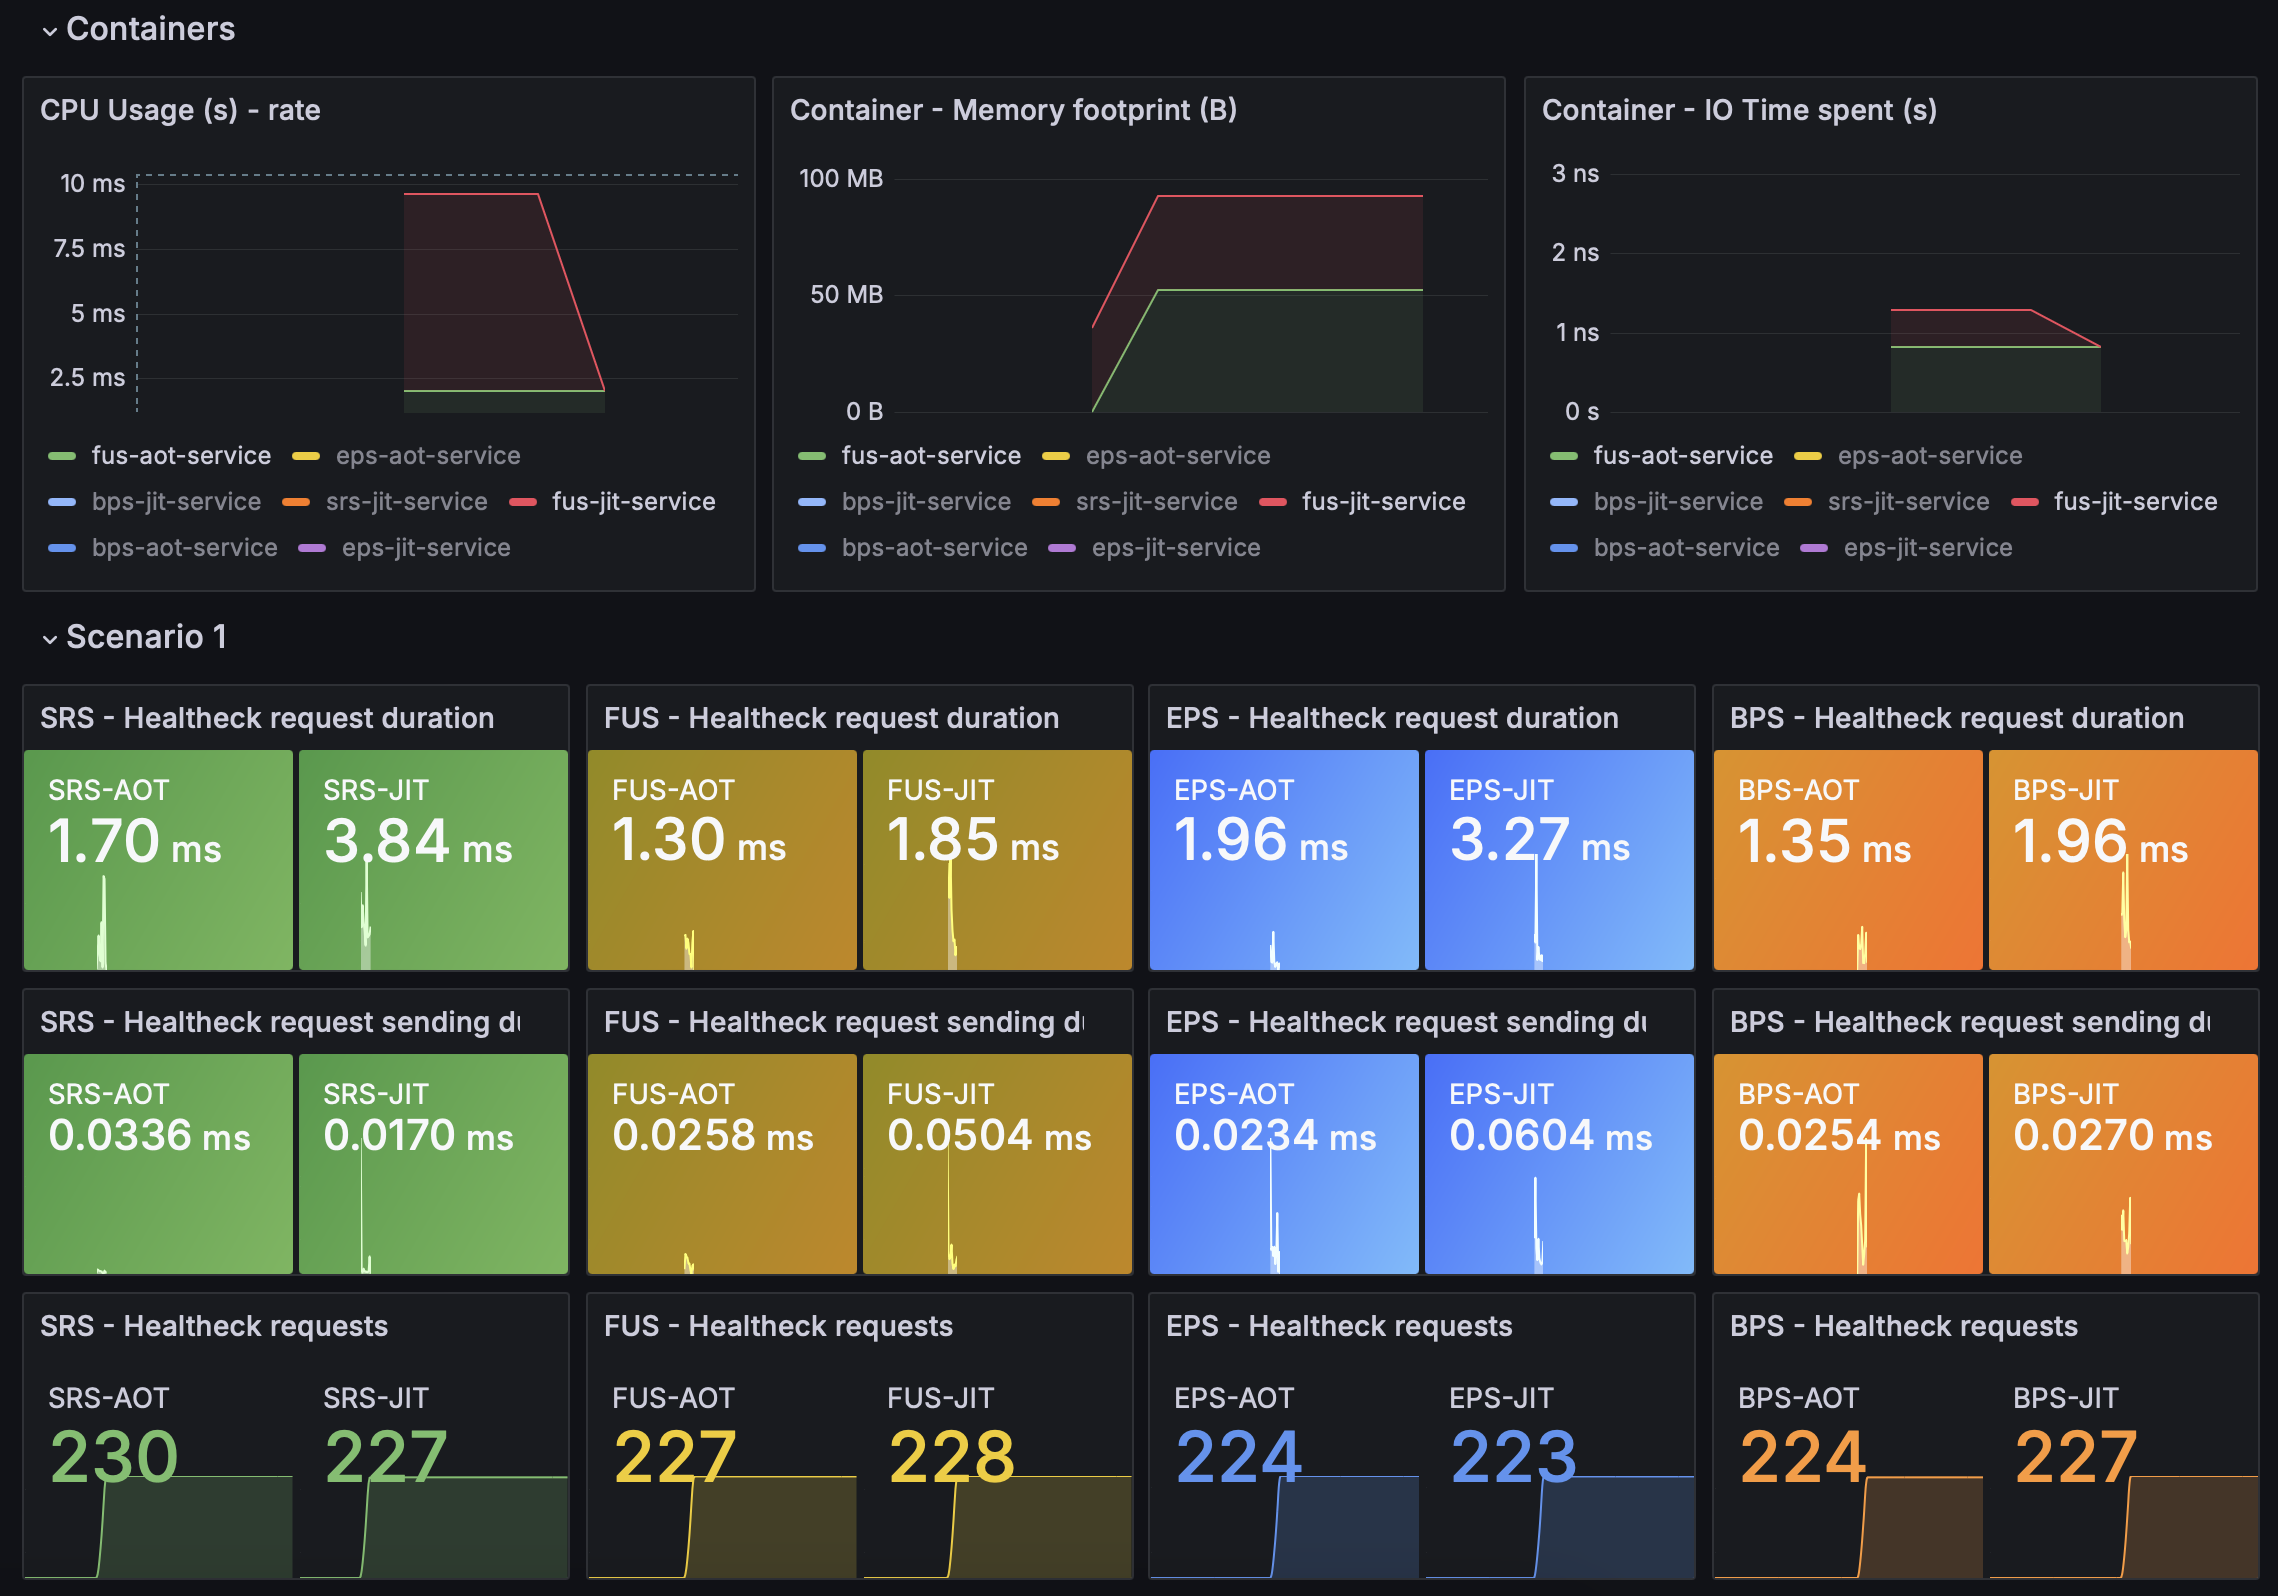
\includegraphics[width=1\textwidth]{graphics/images/scenario1-dashboard.png}
    \caption{Scénář 1 - Grafana dashboard}
    \label{fig:scenario1dashboard}
\end{figure}

% ============================================================================ %
 % Prilohy


% ============================================================================ %

\end{document}

% ============================================================================ %
